% !TeX root=../main.tex

\chapter{مقدمه}
% دستور زیر باعث عدم‌نمایش شماره صفحه در اولین صفحهٔ این فصل می‌شود.
%\thispagestyle{empty}
حروف چینی و قالب‌بندی مناسب برای نوشتن گزارش پروژه، پایان‌نامه یا رسالهٔ‌دکتری امری ضروری است که معمولاً نیازمند صرف زمان بسیار می‌باشد و این مهم نگارنده را از هدف اصلی خود یعنی انتقال دانش به دست آمده، دور می‌کند. نرم‌افزارهای مختلفی برای تدون و نگارش متون وجود دارند که یکی از معروف‌ترین آن‌ها نرم‌افزار ورد%
\LTRfootnote{Word}
از مجموعه نرم‌افزار‌های آفیس می‌باشد. این نرم‌افزار توسط شرکت ماکروسافت توسعه داده شده است و قابلیت استفاده برای نگارش متون مختلف را دارد. اما اگر از این نرم‌افزار برای نگارش \پ استفاده کرده باشید قطعاً متوجه چالش‌های فراوان آن هنگام ایجاد انواع فهرست‌ها، ارجاع به بخش‌های مختلف و ایجاد لیست مراجع شده اید. از این رو توصیه می‌شود برای نگارش چنین متن‌هایی از 
\lr{\LaTeX}
استفاده شود که یک نرم‌افزار کارآمد برای حروف چینی متون است و می‌تواند به صورت خودکار فهرست بندی، ایجاد لیست مراجع، شماره گذاری‌ها، واژه نامه و نمایه را مدیریت کند. حروف‌چینی \پ یکی از موارد پرکاربرد استفاده از
\lr{\LaTeX}
و زی‌پرشین
\cite{Khalighi87xepersian}
است. به علاوه
\lr{\LaTeX}
را می‌توان هم در سیستم عامل ویندوز، هم در سیستم عامل‌های لینوکسی استفاده نمود. این نرم‌افزار قابلیت‌های بسیاری در حروف چینی و ایجاد قالب از طریق ساخت یک فایل کلاس را دارد، از این رو  کلاسی با نام 
\lr{kntu-thesis}
برای حروف‌چینی \پ دانشگاه صتعتی خواجه نصیرالدین طوسی (بر پایه‌ی کلاس
\lr{tehran-thesis}
) آماده نموده ایم که این کلاس مطابق با ستورالعمل نگارش و تدوین پایان‌نامه کارشناسی ارشد و دکتری دانشگاه خواجه نصیرالدین طوسی
\cite{KNTUThesisGuide}
تهیه و تنظیم شده است. 

در ادامه این راهنما ابتدا نحوه‌ی استفاده از این قالب شرح داده می‌شود و سپس نکات لازم برای نوشتن فصل مقدمه بیان می‌گردد. در فصل‌های آتی تنها ویژگی‌های محتوایی که باید در هر فصل شرح داده شود بیان می‌گردد. در پیوست نیز نکات عمومی و دستورات رایج جهت استفاده از لاتک آورده شده است. فایل قالب را می‌توانید از 
\href{https://github.com/msinamsina/kntu-thesis}{لینک گیت‌هاب}
\LTRfootnote{https://github.com/msinamsina/kntu-thesis}
 آن دانلود نمایید و با دادن ستاره  به  پروژه  ما را حمایت کنید. 

\section{نحوه‌ی استفاده از قالب}
این قالب برای استفاده‌ی راحت‌تر از تعدادی فایل و پوشه تشکیل شده است و بر حسب نیاز می‌توان هنگام نگارش
فایل‌های دیگری را نیز به آن اضافه نمود. تمامی فونت‌های مورد استفاده در این قالب در پوشه‌ی 
\lr{font}
همراه با سایر فایل‌های قالب قرار داده شده است و نیاز به نصب جداگانه‌ی فونت‌های استفاده شده نمی‌باشد.
تصاویر در پوشه‌ی 
\lr{img}
قرار دارند و بهتر است برای تصاویر استفاده ‌شده در فصل‌های مختلف پوشه‌های مختلفی در پوشه‌ی
\lr{img}
ایجاد گردد تا از سردرگمی ‌هنگام زیاد شدن تصاویر جلوگیری شود. همچنین توصیه می‌شود تصاویر با فرمت
\lr{PDF}
ذخیره شوند تا کیفیت بالاتر و حجم کمتری داشته باشد.
تمامی فایل‌های متنی که نیاز به ویرایش و بازنویسی توسط نگارنده \پ دارند در پوشه‌ی
\lr{tex}
قرار داده شده‌است. در بخش
\ref{sec:edit}
به طور کامل به کاربرد هر یک از این فایل‌ها پرداخته می‌شود.


\subsection{آماده سازی محیط اجرا}
برای استفاده از این قالب می‌توانید از 
\glspl{Platform}‌ی
\gls{Online}
نظیر 
\lr{\href{https://www.overleaf.com/}{overleaf}}
استفاده کنید و پس از 
\gls{Upload}
فایل 
\lr{zip}
قالب بدون نصب چیزی از آن استفاده کنید.
اما اگر می‌خواهید آن را در رایانه خود اجرا کنید، ابتدا باید یک توزیع تک مناسب بر روی سیستم خود نصب کنید. برای این منظور می‌توانید از تک‌لایو
\lr{(TeXLive)}
استفاده کنید.

برای نصب نسخه‌های مختلف تک‌لایو در ویندوز می‌توانید فایل 
\lr{iso}
آن را از این
\href{https://ftp.math.utah.edu/pub/tex/historic/systems/texlive/}{لینک}%
\LTRfootnote{\lr{\url{https://ftp.math.utah.edu/pub/tex/historic/systems/texlive/}}}
دانلود کنید.
همچنین برای نصب آن در لینوکس می‌توان مستقیماً آن را از مخازن توزیع لینوکس خود بگیرید. به عنوان مثال در اوبونتو می‌توانید با دستور
\LRE{\verb!sudo apt install texlive-full!}
آن را نصب کنید. 
\footnote{
	این قالب با استفاده از
	\lr{TeXLive2022}
	ساخته شده است.}

برای تایپ و ویرایش فایل‌ها علاوه بر نصب لاتک باید یک ویرایشگر مناسب نیز نصب کتید. برای این منظور می‌نوانید از ویرایشگرهایی نظیر
\lr{TeXstudio},
\lr{TeXWroks},
\lr{Texmaker}
و
\lr{BiDiTeXmaker}
استفاده کنید. ویرایش‌گر 
\href{https://bitbucket.org/srazi/biditexmaker3}{\lr{BiDiTeXmaker}}%
\LTRfootnote{\lr{\url{https://bitbucket.org/srazi/biditexmaker3}}}
برای کار با زی‌پرشین و نگارش مطالب دوجهته بهبود یافته است و بهینه‌ترین ویرایشگر لاتک برای کار با اسناد فارسی است. اما ما در ادامه از ویرایشگر 
\lr{TeXstudio}
استفاده می‌کنیم که رایج‌تر است.

\subsection{منابع مناسب برای یادگیری لاتک}
اگر نوشتن \پ اولین تجربه شما از کار با لاتک است، توصیه می‌شود که یک‌بار به صورت اجمالی، کتاب «%
مقدمه‌ای نه چندان کوتاه بر
\lr{\LaTeXe}%
\LTRfootnote{فایل آن در پوشه‌ی قالب قرار داده شده است}»
ترجمه دکتر مهدی امیدعلی را مطالعه کنید. این کتاب، کتاب بسیار کاملی است که خیلی از نیازهای شما در ارتباط با حروف‌چینی را برطرف می‌کند.
اگر تک لایو کامل را داشته باشید، این کتاب را هم دارید. کافیست در خط فرمان دستور زیر را بزنید:
\begin{latin}
	\texttt{texdoc lshort-persian}
\end{latin}
اگر عجله دارید، برخی دستورات پایه‌ای مورد نیاز در پیوست \ref{app:latexIntro} بیان شده‌اند.


\subsection{فونت‌های استفاده شده در قالب}
در این قالب از فونت‌
\lr{IRLotusICEE}
به صورت پیش‌فرض استفاده شده است و بر اساس درستور العمل دانشگاه نباید از فونت
\lr{IRTitr}
برای عنوان استفاده شود.
قلم‌های
\lr{IRLotusICEE}
مستخرج از قلم‌های استاندارد
\lr{IRLotus}
شورای عالی اطلاع‌رسانی%
\footnote{
قلم‌های استاندارد
\lr{IRFonts}
از شورای عالی اطلاع‌رسانی، منطبق بر آخرین نسخه استاندارد یونیکد، استاندارد ملی ۶۲۱۹ و استاندارد
\lr{Adobe Glyph Naming}
هستند.
}
هستند که توسط دکتر بابایی‌زاده اصلاحاتی روی آنها صورت پذیرفته است: تبدیل صفر توپر به صفر توخالی (جهت تمایز بیشتر با نقطه) و اضافه شدن
\textit{\textbf{حالت توپر و ایرانیک توأم}}،
که این موارد در قلم‌های شورای عالی اطلاع‌رسانی وجود ندارد.


\subsection{روش ویراش فایل‌ها}\label{sec:edit}
گزارش پروژه، پایان‌نامه یا رساله، یک نوشته طولانی است که از بخش‌های متعددی تشکیل شده است. بنابراین اگر تمام تنطیمات و مطالب را در یک فایل قرار دهیم، موجب سردرگمی می‌گردد و یافتن بخش‌های مختلف را دشوار می‌کند. برای رفع این مشکل در لاتک می‌توان از فایل‌ها جداگانه برای نگارش بخش‌های مختلف و انجام تنظیمات استفاده نمود و سپس همه‌ی آن‌ها را در فایل اصلی فراخوانی نمود.
در قالب تهیه‌شده توسط ما  
\textbf{
	فایل اصلی مجموعه،
	\lr{main.tex}
	می‌باشد.
}
که قسمت‌های مختلف، توسط دستورهایی مانند 
\lr{input}
و
\lr{include}
در این فایل فراخوانی شده‌اند.
برای درک بهتر فایل‌های مختلف فراخوانی شده در
\lr{main.tex}،
در این بخش به توضیح مختصر هر یک پرداخته می‌شود.

\begin{itemize}
	\item \lr{kntu-thesis.cls}: 
	در این فایل تنظیمات پایه‌ای قالب قرار داده شده است 
	و توصیه می‌شود اگر در استفاده از لاتک تازه‌کار هستید
	این فایل را تغییر ندهید.
	\item \lr{commands.tex}:
	در این فایل تنظیمات قابل تغییر توسط کاربر قرار داده شده است.
	اگر در هنگام نگارش به پکیج جدیدی نیاز داشتید که از پیش در قالب
	فراخوانی نشده بود لازم است آن‌ها در این فایل فراخوانی شوند. همچنین 
	در صورتی که می‌خواهید از فونت‌های جدید نیز  استفاده کنید علاوه بر اضافه
	کردن فاید فوند در پوشه‌ی
	\lr{font}
	یاید در به این فایل نیز فونت مورد نظر تعریف گردد. در این فایل عبارت 
	"فونت‌های جدید" را جست و جو نمایید و بر اساس مثال هایی که در آنجا قرار
	داده شده است، فونت‌های جدید را وارد نمایید.
	\item \lr{faTitle.tex}:
	در این فایل مشخصات فارسی نظیر عنوان، نام نگارنده و 
	اساتید راهنما به همراه چکیده فارسی قرار دارد 
	که باید توسط کاربر تغییر کند. در این فایل در صورت
	نداشتن گرایش، استاد مشاور و یا استاد راهنمای دوم هر
	یک از این موارد را با قرار دادن کاراکتر
	\%
	در ابتدای آن خط کامنت کنید. لازم به ذکر است که تنظیمات
	موجود در فایل
	\lr{kntu-thesis.cls}
	به گونه‌ای است که کاربر فقط یک با مشخصات خود و عنوان
	را وارد کند و اطلاعات لازم به صورت خودکار در بخش‌های 
	مختلف قرار می‌گیرد. 
	\item \lr{enTitle.tex}:
	همانند فایل
	\lr{faTitle.tex}
	اما برای مشخصات و چکیده‌ی انگیسی می‌باشد.
	\item \lr{glossaries-settings.tex}
	و
	\lr{words.tex}:
	این دو فایل برای ایجاد واژه‌نامه استفاده می‌شوند.
	برای ایجاد واژه نامه از پکیج 
	\lr{glossary}
	استفاده شده است و	تنظیمات آن در فایل
	\lr{glossaries-settings.tex}
	قرار دارد و نیازی به نغییر این فایل توسط کاریر نمی‌باشد.
	اما واژه‌های معادلی که برای واژه‌های انگلیسی استفاده شده
	است را باید در فایل  
	\lr{words.tex}
	اضافه کنیم. لازم به ذکر است که ایجاد واژه نامه و نمایه 
	طبق دستورالعمل دانشگاه اجباری نیست و در صورتی که نمی‌خواهید
	واژه نامه و نمایه در \پ داشته باشید می‌توان خطوط مربوط به 
	 \lr{glossaries-settings.tex}
	و
	\lr{words.tex}
	را
	در فایل 
	\lr{main.tex}
	کامنت و یا حذف نمایید.
	\item \lr{thesis\_preamble.tex}:
	این فایل جهت تنظیم صفحات ابتدایی استفاده می‌شود به
	عنوان مثال اگر	قصد دارید صفحات تفدیم و یا قدردانی
	را حذف کنید می‌توانید دستورات	مربوط به آن را در این
	فایل کامنت کنید. نمایش موادی نظیر فهرست برنامه‌ها، 
	فهرست الگوریتم‌ها و فهرست اختصارات نیز در این فایل
	انجام می‌شود. که در صورت تمایل می‌توانید آن‌ها را حذف
	نمایید.
	\item \lr{MyReferences.bib}:
	این فایل برای مدیریت مراجع استفاده می‌شود. می‌توانید
	با جست‌و‌جوی مقالات مورد نظر در 
	\lr{\href{https://scholar.google.com/}{Google Scholar}}
	محتوای
	\lr{bib.tex}
	آن‌ها کپی و در فایل
	\lr{MyReferences.bib}
	قرار دهید و سپس در متن خود با دستور
	\verb*|\cite{lable}|
	به آن ارجاع دهید. برای توضیحات کامل تر به بخش
	\ref{app:bibref}
	در پیوست ها مراجعه کنید.
	این قالب ترتیب مراجع را به
	صورت خودکار مدیریت می‌کند و از استاندارد ‌IEEE 
	برای این کار استفاده می‌کند.
	
	\item
	 فایل‌های فصل‌ها و پیوست‌ها: به صورت پیش‌فرض پنچ
	 فصل و سه پیوست در این قالب قرار داده شده است.
	 اما کاربر می‌تواند به دلخواه خود و صلاح دید استاد
	 راهنما این موارد را کم یا زیاد کند. به عنوان 
	 مثال اگر بخواهید یک فصل دیگر اضافه کند می‌تواند
	 یک فایل با نامی دلخواه مثل
	 \verb*|chapter6.tex|
	 ایجاد کند و آن را در پوشه‌ی 
	 \lr{tex}
	 سپس با دستور
	 \verb*|\include{./tex/chapter6}|
	آن را در ادامه‌‌ی سایر فصل‌ها قرار دهد و یا در صورتی
	که نیازی به پیوست نداشته باشد می‌تواند دستورات مربوط
	به آن را در فایل 
	\lr{main.tex}
	کامنت کند.
\end{itemize}
	\subsection[مطالب پایان‌نامه را چطور بنویسم؟]
	{نوشتن محتوای اصلی}
در ویرایش فایل‌ها باید به این نکته توجه شود که دستورات موجود در آن‌ها ناآگاهانه حذف نگردد چراکه ممکن است باعث ایجاد خطا در هنگام اجرا شود.
نکته دیگری که باید به آن توجه کنید این است که در قالب آماده شده، سه گزینه به نام‌های
\lr{bsc}،
\lr{msc}
و
\lr{phd}
برای نوشتن پروژه، پایان‌نامه و رساله، در نظر گرفته شده است. بنابراین اگر قصد تایپ پروژهٔ کارشناسی، پایان‌نامهٔ کارشناسی ارشد یا رسالهٔ دکتری را دارید، به ترتیب باید از گزینه‌های
\lr{bsc}،
\lr{msc}
و
\lr{phd}
در فایل 
\lr{main.tex}
استفاده کنید. با انتخاب هر کدام از این گزینه‌ها، تنظیمات مربوط به آنها به طور خودکار، اعمال می‌شود.
	\subsubsection{فصل‌ها}

برای ویرایش هر فصل می‌توانید فایل مربوط به آن فصل را باز نموده و مطالب خود را با مطالب فعلی جایگزین کنید. نکته بسیار مهمی که در اینجا باید گفته شود این است که سیستم \lr{\TeX}، محتویات یک فایل تِک را به ترتیب پردازش می‌کند.  بنابراین، اگر مثلاً  دو فصل اول خود را نوشته و خروجی آنها را دیده‌اید و مشغول تایپ مطالب فصل ۳ هستید، بهتر است
	که دو دستور 
	\verb!% !TeX root=../main.tex

\chapter{مقدمه}
% دستور زیر باعث عدم‌نمایش شماره صفحه در اولین صفحهٔ این فصل می‌شود.
%\thispagestyle{empty}
حروف چینی و قالب‌بندی مناسب برای نوشتن گزارش پروژه، پایان‌نامه یا رسالهٔ‌دکتری امری ضروری است که معمولاً نیازمند صرف زمان بسیار می‌باشد و این مهم نگارنده را از هدف اصلی خود یعنی انتقال دانش به دست آمده، دور می‌کند. نرم‌افزارهای مختلفی برای تدون و نگارش متون وجود دارند که یکی از معروف‌ترین آن‌ها نرم‌افزار ورد%
\LTRfootnote{Word}
از مجموعه نرم‌افزار‌های آفیس می‌باشد. این نرم‌افزار توسط شرکت ماکروسافت توسعه داده شده است و قابلیت استفاده برای نگارش متون مختلف را دارد. اما اگر از این نرم‌افزار برای نگارش \پ استفاده کرده باشید قطعاً متوجه چالش‌های فراوان آن هنگام ایجاد انواع فهرست‌ها، ارجاع به بخش‌های مختلف و ایجاد لیست مراجع شده اید. از این رو توصیه می‌شود برای نگارش چنین متن‌هایی از 
\lr{\LaTeX}
استفاده شود که یک نرم‌افزار کارآمد برای حروف چینی متون است و می‌تواند به صورت خودکار فهرست بندی، ایجاد لیست مراجع، شماره گذاری‌ها، واژه نامه و نمایه را مدیریت کند. حروف‌چینی \پ یکی از موارد پرکاربرد استفاده از
\lr{\LaTeX}
و زی‌پرشین
\cite{Khalighi87xepersian}
است. به علاوه
\lr{\LaTeX}
را می‌توان هم در سیستم عامل ویندوز، هم در سیستم عامل‌های لینوکسی استفاده نمود. این نرم‌افزار قابلیت‌های بسیاری در حروف چینی و ایجاد قالب از طریق ساخت یک فایل کلاس را دارد، از این رو  کلاسی با نام 
\lr{kntu-thesis}
برای حروف‌چینی \پ دانشگاه صتعتی خواجه نصیرالدین طوسی (بر پایه‌ی کلاس
\lr{tehran-thesis}
) آماده نموده ایم که این کلاس مطابق با ستورالعمل نگارش و تدوین پایان‌نامه کارشناسی ارشد و دکتری دانشگاه خواجه نصیرالدین طوسی
\cite{KNTUThesisGuide}
تهیه و تنظیم شده است. 

در ادامه این راهنما ابتدا نحوه‌ی استفاده از این قالب شرح داده می‌شود و سپس نکات لازم برای نوشتن فصل مقدمه بیان می‌گردد. در فصل‌های آتی تنها ویژگی‌های محتوایی که باید در هر فصل شرح داده شود بیان می‌گردد. در پیوست نیز نکات عمومی و دستورات رایج جهت استفاده از لاتک آورده شده است.

\section{نحوه‌ی استفاده از قالب}
این قالب برای استفاده‌ی راحت‌تر از تعدادی فایل و پوشه تشکیل شده است و بر حسب نیاز می‌توان هنگام نگارش
فایل‌های دیگری را نیز به آن اضافه نمود. تمامی فونت‌های مورد استفاده در این قالب در پوشه‌ی 
\lr{font}
همراه با سایر فایل‌های قالب قرار داده شده است و نیاز به نصب جداگانه‌ی فونت‌های استفاده شده نمی‌باشد.
تصاویر در پوشه‌ی 
\lr{img}
قرار دارند و بهتر است برای تصاویر استفاده ‌شده در فصل‌های مختلف پوشه‌های مختلفی در پوشه‌ی
\lr{img}
ایجاد گردد تا از سردرگمی ‌هنگام زیاد شدن تصاویر جلوگیری شود. همچنین توصیه می‌شود تصاویر با فرمت
\lr{PDF}
ذخیره شوند تا کیفیت بالاتر و حجم کمتری داشته باشد.
تمامی فایل‌های متنی که نیاز به ویرایش و بازنویسی توسط نگارنده \پ دارند در پوشه‌ی
\lr{tex}
قرار داده شده‌است. در بخش
\ref{sec:edit}
به طور کامل به کاربرد هر یک از این فایل‌ها پرداخته می‌شود.

\subsection{فونت‌های استفاده شده در قالب}
در این قالب از فونت‌های
\lr{IRLotusICEE}
 و
\lr{IRTitr}
استفاده شده است.
قلم‌های
\lr{IRLotusICEE}
مستخرج از قلم‌های استاندارد
\lr{IRLotus}
شورای عالی اطلاع‌رسانی%
\footnote{
قلم‌های استاندارد
\lr{IRFonts}
از شورای عالی اطلاع‌رسانی، منطبق بر آخرین نسخه استاندارد یونیکد، استاندارد ملی ۶۲۱۹ و استاندارد
\lr{Adobe Glyph Naming}
هستند.
}
هستند که توسط دکتر بابایی‌زاده اصلاحاتی روی آنها صورت پذیرفته است: تبدیل صفر توپر به صفر توخالی (جهت تمایز بیشتر با نقطه) و اضافه شدن
\textit{\textbf{حالت توپر و ایرانیک توأم}}،
که این موارد در قلم‌های شورای عالی اطلاع‌رسانی وجود ندارد.


\subsection{روش ویراش فایل‌ها}\label{sec:edit}
گزارش پروژه، پایان‌نامه یا رساله، یک نوشته طولانی است که از بخش‌های متعددی تشکیل شده است. بنابراین اگر تمام تنطیمات و مطالب را در یک فایل قرار دهیم، موجب سردرگمی می‌گردد و یافتن بخش‌های مختلف را دشوار می‌کند. برای رفع این مشکل در لاتک می‌توان از فایل‌ها جداگانه برای نگارش بخش‌های مختلف و انجام تنظیمات استفاده نمود و سپس همه‌ی آن‌ها را در فایل اصلی فراخوانی نمود.
در قالب تهیه‌شده توسط ما  
\textbf{
	فایل اصلی مجموعه،
	\lr{main.tex}
	می‌باشد.
}
که قسمت‌های مختلف، توسط دستورهایی مانند 
\lr{input}
و
\lr{include}
در این فایل فراخوانی شده‌اند.
برای درک بهتر فایل‌های مختلف فراخوانی شده در
\lr{main.tex}،
در این بخش به توضیح مختصر هر یک پرداخته می‌شود.

\begin{itemize}
	\item \lr{kntu-thesis.cls}: 
	در این فایل تنظیمات پایه‌ای قالب قرار داده شده است 
	و توصیه می‌شود اگر در استفاده از لاتک تازه‌کار هستید
	این فایل را تغییر ندهید.
	\item \lr{commands.tex}:
	در این فایل تنظیمات قابل تغییر توسط کاربر قرار داده شده است.
	اگر در هنگام نگارش به پکیج جدیدی نیاز داشتید که از پیش در قالب
	فراخوانی نشده بود آن‌ها را در این فایل اضافه شود. همچنین فونت‌های
	جدید نیز یاید به این فایل اضافه شود.
	\item \lr{faTitle.tex}:
	در این فایل مشخصات فارسی نظیر عنوان، نام نگارنده و 
	اساتید راهنما به همراه چکیده فارسی قرار دارد 
	که باید توسط کاربر تغییر کند. در این فایل در صورت
	نداشتن گرایش، استاد مشاور و یا استاد راهنمای دوم هر
	یک از این موارد را با قرار دادن کاراکتر
	\%
	در ابتدای آن خط کامنت کنید. لازم به ذکر است که تنظیمات
	موجود در فایل
	\lr{kntu-thesis.cls}
	به گونه‌ای است که کاربر فقط یک با مشخصات خود و عنوان
	را وارد کند و اطلاعات لازم به صورت خودکار در بخش‌های 
	مختلف قرار می‌گیرد. 
	\item \lr{enTitle.tex}:
	همانند فایل
	\lr{faTitle.tex}
	اما برای مشخصات و چکیده‌ی انگیسی می‌باشد.
	\item \lr{glossaries-settings.tex}
	و
	\lr{words.tex}:
	این دو فایل برای ایجاد واژه‌نامه استفاده می‌شوند.
	تنظیمات پکیج استفاده شده جهت ایجاد واژه نامه در فایل
	\lr{glossaries-settings.tex}
	قرار دارد و نیازی به نغییر این فایل توسط کاریر نمی‌باشد.
	اما واژه‌های معادلی که برای واژه‌های انگلیسی استفاده شده
	است را باید در فایل  
	\lr{words.tex}
	اضافه کنیم.
	\item \lr{thesis\_preamble.tex}:
	این فایل جهت تنظیم صفحات ابتدایی استفاده می‌شود به
	عنوان مثال اگر	قصد دارید صفحات تفدیم و یا قدردانی
	را حذف کنید می‌توانید دستورات	مربوط به آن را در این
	فایل کامنت کنید.
	\item \lr{MyReferences.bib}:
	این فایل برای مدیریت مراجع استفاده می‌شود. می‌توانید
	با جست‌و‌جوی مقالات مورد نظر در 
	\lr{\href{https://scholar.google.com/}{Google Scholar}}
	محتوای
	\lr{bib.tex}
	آن‌ها کپی و در فایل
	\lr{MyReferences.bib}
	قرار دهید و سپس در متن خود با دستور
	\verb*|\cite{lable}|
	به آن ارجاع دهید. این قالب ترتیب مراجع را به
	صورت خودکار مدیریت می‌کند و از استاندارد ‌IEEE 
	برای این کار استفاده می‌کند.
	
	\item
	 فایل‌های فصل‌ها و پیوست‌ها: به صورت پیش‌فرض پنچ
	 فصل و سه پیوست در این قالب قرار داده شده است.
	 اما کاربر می‌تواند به دلخواه خود و صلاح دید استاد
	 راهنما این موارد را کم یا زیاد کند. به عنوان 
	 مثال اگر بخواهید یک فصل دیگر اضافه کند می‌تواند
	 یک فایل با نامی دلخواه مثل
	 \verb*|chapter6.tex|
	 ایجاد کند و آن را در پوشه‌ی 
	 \lr{tex}
	 سپس با دستور
	 \verb*|\include{./tex/chapter6}|
	آن را در ادامه‌‌ی سایر فصل‌ها قرار دهد و یا در صورتی
	که نیازی به پیوست نداشته باشد می‌تواند دستورات مربوط
	به آن را در فایل 
	\lr{main.tex}
	کامنت کند.

\end{itemize}

در ویرایش فایل‌ها باید به این نکته توجه شود که دستورات موجود در آن‌ها ناآگاهانه حذف نگردد چراکه ممکن است باعث ایجاد خطا در هنگام اجرا شود.
نکته دیگری که باید به آن توجه کنید این است که در قالب آماده شده، سه گزینه به نام‌های
\lr{bsc}،
\lr{msc}
و
\lr{phd}
برای نوشتن پروژه، پایان‌نامه و رساله، در نظر گرفته شده است. بنابراین اگر قصد تایپ پروژهٔ کارشناسی، پایان‌نامهٔ کارشناسی ارشد یا رسالهٔ دکتری را دارید، به ترتیب باید از گزینه‌های
\lr{bsc}،
\lr{msc}
و
\lr{phd}
در فایل 
\lr{main.tex}
استفاده کنید. با انتخاب هر کدام از این گزینه‌ها، تنظیمات مربوط به آنها به طور خودکار، اعمال می‌شود.
 
\subsection{آماده سازی محیط اجرا}
برای استفاده از این قالب ابتدا باید یک توزیع تک مناسب بر روی سیستم خود نصب کنید. برای این منظور می‌توانید از تک‌لایو
\lr{(TeXLive)}
استفاده کنید.

برای نصب نسخه‌های مختلف تک‌لایو در ویندوز می‌توانید فایل 
\lr{iso}
آن را از این
 \href{https://ftp.math.utah.edu/pub/tex/historic/systems/texlive/}{لینک}%
\LTRfootnote{\lr{\url{https://ftp.math.utah.edu/pub/tex/historic/systems/texlive/}}}
دانلود کنید.
همچنین برای نصب آن در لینوکس می‌توان مستقیماً آن را از مخازن توزیع لینوکس خود بگیرید. به عنوان مثال در اوبونتو می‌توانید با دستور
\LRE{\verb!sudo apt install texlive-full!}
آن را نصب کنید.

برای تایپ و ویرایش فایل‌ها علاوه بر نصب لاتک باید یک ویرایشگر مناسب نیز نصب کتید. برای این منظور می‌نوانید از ویرایشگرهایی نظیر
\lr{TeXstudio},
\lr{TeXWroks},
\lr{Texmaker}
و
\lr{BiDiTeXmaker}
استفاده کنید. ویرایش‌گر 
 \href{https://bitbucket.org/srazi/biditexmaker3}{\lr{BiDiTeXmaker}}%
 \LTRfootnote{\lr{\url{https://bitbucket.org/srazi/biditexmaker3}}}
برای کار با زی‌پرشین و نگارش مطالب دوجهته بهبود یافته است و بهینه‌ترین ویرایشگر لاتک برای کار با اسناد فارسی است. اما ما در ادامه از ویرایشگر 
\lr{TeXstudio}
استفاده می‌کنیم که رایج‌تر است.

\subsection{منابع مناسب برای یادگیری لاتک}
اگر نوشتن \پ اولین تجربه شما از کار با لاتک است، توصیه می‌شود که یک‌بار به صورت اجمالی، کتاب «%
مقدمه‌ای نه چندان کوتاه بر
\lr{\LaTeXe}%
\LTRfootnote{فایل آن در پوشه‌ی قالب قرار داده شده است}»
ترجمه دکتر مهدی امیدعلی را مطالعه کنید. این کتاب، کتاب بسیار کاملی است که خیلی از نیازهای شما در ارتباط با حروف‌چینی را برطرف می‌کند.
اگر تک لایو کامل را داشته باشید، این کتاب را هم دارید. کافیست در خط فرمان دستور زیر را بزنید:
\begin{latin}
	\texttt{texdoc lshort-persian}
\end{latin}
اگر عجله دارید، برخی دستورات پایه‌ای مورد نیاز در پیوست \ref{app:latexIntro} بیان شده‌اند.

\subsection[مطالب پایان‌نامه را چطور بنویسم؟]
{مطالب \پ را چطور بنویسم؟}
\subsubsection{نوشتن فصل‌ها}
همان‌طور که در بخش \ref{sec:edit} گفته شد برای جلوگیری از شلوغی، قسمت‌های مختلف \پ از جمله فصل‌ها، در فایل‌های جداگانه‌ای قرار داده شده‌اند. 
مثلاً اگر می‌خواهید مطالب فصل ۱ را تایپ کنید، باید فایل‌های 
\lr{main.tex}
و
\lr{chapter1.tex}
را باز کرده و مطالب خود را جایگزین محتویات داخل 
\lr{chapter1.tex}
نمایید. دقت شود که در ابتدای برخی فایلها دستوراتی نوشته شده است و از شما خواسته شده که آن دستورات را حذف نکنید.

%توجه کنید که همان‌طور که قبلاً هم گفته شد، تنها فایل قابل اجرا، 
%\lr{main.tex}
%است. لذا برای دیدن حاصل (خروجی) فایل خود، باید  
%\lr{chapter1.tex}
%را ذخیره کرده و سپس فایل 
%\lr{main.tex}
%را اجرا کنید.

نکته بسیار مهمی که در اینجا باید گفته شود این است که سیستم \lr{\TeX}، محتویات یک فایل تِک را به ترتیب پردازش می‌کند.  بنابراین، اگر مثلاً  دو فصل اول خود را نوشته و خروجی آنها را دیده‌اید و مشغول تایپ مطالب فصل ۳ هستید، بهتر است
که دو دستور 
\verb!% !TeX root=../main.tex

\chapter{مقدمه}
% دستور زیر باعث عدم‌نمایش شماره صفحه در اولین صفحهٔ این فصل می‌شود.
%\thispagestyle{empty}
حروف چینی و قالب‌بندی مناسب برای نوشتن گزارش پروژه، پایان‌نامه یا رسالهٔ‌دکتری امری ضروری است که معمولاً نیازمند صرف زمان بسیار می‌باشد و این مهم نگارنده را از هدف اصلی خود یعنی انتقال دانش به دست آمده، دور می‌کند. نرم‌افزارهای مختلفی برای تدون و نگارش متون وجود دارند که یکی از معروف‌ترین آن‌ها نرم‌افزار ورد%
\LTRfootnote{Word}
از مجموعه نرم‌افزار‌های آفیس می‌باشد. این نرم‌افزار توسط شرکت ماکروسافت توسعه داده شده است و قابلیت استفاده برای نگارش متون مختلف را دارد. اما اگر از این نرم‌افزار برای نگارش \پ استفاده کرده باشید قطعاً متوجه چالش‌های فراوان آن هنگام ایجاد انواع فهرست‌ها، ارجاع به بخش‌های مختلف و ایجاد لیست مراجع شده اید. از این رو توصیه می‌شود برای نگارش چنین متن‌هایی از 
\lr{\LaTeX}
استفاده شود که یک نرم‌افزار کارآمد برای حروف چینی متون است و می‌تواند به صورت خودکار فهرست بندی، ایجاد لیست مراجع، شماره گذاری‌ها، واژه نامه و نمایه را مدیریت کند. حروف‌چینی \پ یکی از موارد پرکاربرد استفاده از
\lr{\LaTeX}
و زی‌پرشین
\cite{Khalighi87xepersian}
است. به علاوه
\lr{\LaTeX}
را می‌توان هم در سیستم عامل ویندوز، هم در سیستم عامل‌های لینوکسی استفاده نمود. این نرم‌افزار قابلیت‌های بسیاری در حروف چینی و ایجاد قالب از طریق ساخت یک فایل کلاس را دارد، از این رو  کلاسی با نام 
\lr{kntu-thesis}
برای حروف‌چینی \پ دانشگاه صتعتی خواجه نصیرالدین طوسی (بر پایه‌ی کلاس
\lr{tehran-thesis}
) آماده نموده ایم که این کلاس مطابق با ستورالعمل نگارش و تدوین پایان‌نامه کارشناسی ارشد و دکتری دانشگاه خواجه نصیرالدین طوسی
\cite{KNTUThesisGuide}
تهیه و تنظیم شده است. 

در ادامه این راهنما ابتدا نحوه‌ی استفاده از این قالب شرح داده می‌شود و سپس نکات لازم برای نوشتن فصل مقدمه بیان می‌گردد. در فصل‌های آتی تنها ویژگی‌های محتوایی که باید در هر فصل شرح داده شود بیان می‌گردد. در پیوست نیز نکات عمومی و دستورات رایج جهت استفاده از لاتک آورده شده است.

\section{نحوه‌ی استفاده از قالب}
این قالب برای استفاده‌ی راحت‌تر از تعدادی فایل و پوشه تشکیل شده است و بر حسب نیاز می‌توان هنگام نگارش
فایل‌های دیگری را نیز به آن اضافه نمود. تمامی فونت‌های مورد استفاده در این قالب در پوشه‌ی 
\lr{font}
همراه با سایر فایل‌های قالب قرار داده شده است و نیاز به نصب جداگانه‌ی فونت‌های استفاده شده نمی‌باشد.
تصاویر در پوشه‌ی 
\lr{img}
قرار دارند و بهتر است برای تصاویر استفاده ‌شده در فصل‌های مختلف پوشه‌های مختلفی در پوشه‌ی
\lr{img}
ایجاد گردد تا از سردرگمی ‌هنگام زیاد شدن تصاویر جلوگیری شود. همچنین توصیه می‌شود تصاویر با فرمت
\lr{PDF}
ذخیره شوند تا کیفیت بالاتر و حجم کمتری داشته باشد.
تمامی فایل‌های متنی که نیاز به ویرایش و بازنویسی توسط نگارنده \پ دارند در پوشه‌ی
\lr{tex}
قرار داده شده‌است. در بخش
\ref{sec:edit}
به طور کامل به کاربرد هر یک از این فایل‌ها پرداخته می‌شود.

\subsection{فونت‌های استفاده شده در قالب}
در این قالب از فونت‌های
\lr{IRLotusICEE}
 و
\lr{IRTitr}
استفاده شده است.
قلم‌های
\lr{IRLotusICEE}
مستخرج از قلم‌های استاندارد
\lr{IRLotus}
شورای عالی اطلاع‌رسانی%
\footnote{
قلم‌های استاندارد
\lr{IRFonts}
از شورای عالی اطلاع‌رسانی، منطبق بر آخرین نسخه استاندارد یونیکد، استاندارد ملی ۶۲۱۹ و استاندارد
\lr{Adobe Glyph Naming}
هستند.
}
هستند که توسط دکتر بابایی‌زاده اصلاحاتی روی آنها صورت پذیرفته است: تبدیل صفر توپر به صفر توخالی (جهت تمایز بیشتر با نقطه) و اضافه شدن
\textit{\textbf{حالت توپر و ایرانیک توأم}}،
که این موارد در قلم‌های شورای عالی اطلاع‌رسانی وجود ندارد.


\subsection{روش ویراش فایل‌ها}\label{sec:edit}
گزارش پروژه، پایان‌نامه یا رساله، یک نوشته طولانی است که از بخش‌های متعددی تشکیل شده است. بنابراین اگر تمام تنطیمات و مطالب را در یک فایل قرار دهیم، موجب سردرگمی می‌گردد و یافتن بخش‌های مختلف را دشوار می‌کند. برای رفع این مشکل در لاتک می‌توان از فایل‌ها جداگانه برای نگارش بخش‌های مختلف و انجام تنظیمات استفاده نمود و سپس همه‌ی آن‌ها را در فایل اصلی فراخوانی نمود.
در قالب تهیه‌شده توسط ما  
\textbf{
	فایل اصلی مجموعه،
	\lr{main.tex}
	می‌باشد.
}
که قسمت‌های مختلف، توسط دستورهایی مانند 
\lr{input}
و
\lr{include}
در این فایل فراخوانی شده‌اند.
برای درک بهتر فایل‌های مختلف فراخوانی شده در
\lr{main.tex}،
در این بخش به توضیح مختصر هر یک پرداخته می‌شود.

\begin{itemize}
	\item \lr{kntu-thesis.cls}: 
	در این فایل تنظیمات پایه‌ای قالب قرار داده شده است 
	و توصیه می‌شود اگر در استفاده از لاتک تازه‌کار هستید
	این فایل را تغییر ندهید.
	\item \lr{commands.tex}:
	در این فایل تنظیمات قابل تغییر توسط کاربر قرار داده شده است.
	اگر در هنگام نگارش به پکیج جدیدی نیاز داشتید که از پیش در قالب
	فراخوانی نشده بود آن‌ها را در این فایل اضافه شود. همچنین فونت‌های
	جدید نیز یاید به این فایل اضافه شود.
	\item \lr{faTitle.tex}:
	در این فایل مشخصات فارسی نظیر عنوان، نام نگارنده و 
	اساتید راهنما به همراه چکیده فارسی قرار دارد 
	که باید توسط کاربر تغییر کند. در این فایل در صورت
	نداشتن گرایش، استاد مشاور و یا استاد راهنمای دوم هر
	یک از این موارد را با قرار دادن کاراکتر
	\%
	در ابتدای آن خط کامنت کنید. لازم به ذکر است که تنظیمات
	موجود در فایل
	\lr{kntu-thesis.cls}
	به گونه‌ای است که کاربر فقط یک با مشخصات خود و عنوان
	را وارد کند و اطلاعات لازم به صورت خودکار در بخش‌های 
	مختلف قرار می‌گیرد. 
	\item \lr{enTitle.tex}:
	همانند فایل
	\lr{faTitle.tex}
	اما برای مشخصات و چکیده‌ی انگیسی می‌باشد.
	\item \lr{glossaries-settings.tex}
	و
	\lr{words.tex}:
	این دو فایل برای ایجاد واژه‌نامه استفاده می‌شوند.
	تنظیمات پکیج استفاده شده جهت ایجاد واژه نامه در فایل
	\lr{glossaries-settings.tex}
	قرار دارد و نیازی به نغییر این فایل توسط کاریر نمی‌باشد.
	اما واژه‌های معادلی که برای واژه‌های انگلیسی استفاده شده
	است را باید در فایل  
	\lr{words.tex}
	اضافه کنیم.
	\item \lr{thesis\_preamble.tex}:
	این فایل جهت تنظیم صفحات ابتدایی استفاده می‌شود به
	عنوان مثال اگر	قصد دارید صفحات تفدیم و یا قدردانی
	را حذف کنید می‌توانید دستورات	مربوط به آن را در این
	فایل کامنت کنید.
	\item \lr{MyReferences.bib}:
	این فایل برای مدیریت مراجع استفاده می‌شود. می‌توانید
	با جست‌و‌جوی مقالات مورد نظر در 
	\lr{\href{https://scholar.google.com/}{Google Scholar}}
	محتوای
	\lr{bib.tex}
	آن‌ها کپی و در فایل
	\lr{MyReferences.bib}
	قرار دهید و سپس در متن خود با دستور
	\verb*|\cite{lable}|
	به آن ارجاع دهید. این قالب ترتیب مراجع را به
	صورت خودکار مدیریت می‌کند و از استاندارد ‌IEEE 
	برای این کار استفاده می‌کند.
	
	\item
	 فایل‌های فصل‌ها و پیوست‌ها: به صورت پیش‌فرض پنچ
	 فصل و سه پیوست در این قالب قرار داده شده است.
	 اما کاربر می‌تواند به دلخواه خود و صلاح دید استاد
	 راهنما این موارد را کم یا زیاد کند. به عنوان 
	 مثال اگر بخواهید یک فصل دیگر اضافه کند می‌تواند
	 یک فایل با نامی دلخواه مثل
	 \verb*|chapter6.tex|
	 ایجاد کند و آن را در پوشه‌ی 
	 \lr{tex}
	 سپس با دستور
	 \verb*|\include{./tex/chapter6}|
	آن را در ادامه‌‌ی سایر فصل‌ها قرار دهد و یا در صورتی
	که نیازی به پیوست نداشته باشد می‌تواند دستورات مربوط
	به آن را در فایل 
	\lr{main.tex}
	کامنت کند.

\end{itemize}

در ویرایش فایل‌ها باید به این نکته توجه شود که دستورات موجود در آن‌ها ناآگاهانه حذف نگردد چراکه ممکن است باعث ایجاد خطا در هنگام اجرا شود.
نکته دیگری که باید به آن توجه کنید این است که در قالب آماده شده، سه گزینه به نام‌های
\lr{bsc}،
\lr{msc}
و
\lr{phd}
برای نوشتن پروژه، پایان‌نامه و رساله، در نظر گرفته شده است. بنابراین اگر قصد تایپ پروژهٔ کارشناسی، پایان‌نامهٔ کارشناسی ارشد یا رسالهٔ دکتری را دارید، به ترتیب باید از گزینه‌های
\lr{bsc}،
\lr{msc}
و
\lr{phd}
در فایل 
\lr{main.tex}
استفاده کنید. با انتخاب هر کدام از این گزینه‌ها، تنظیمات مربوط به آنها به طور خودکار، اعمال می‌شود.
 
\subsection{آماده سازی محیط اجرا}
برای استفاده از این قالب ابتدا باید یک توزیع تک مناسب بر روی سیستم خود نصب کنید. برای این منظور می‌توانید از تک‌لایو
\lr{(TeXLive)}
استفاده کنید.

برای نصب نسخه‌های مختلف تک‌لایو در ویندوز می‌توانید فایل 
\lr{iso}
آن را از این
 \href{https://ftp.math.utah.edu/pub/tex/historic/systems/texlive/}{لینک}%
\LTRfootnote{\lr{\url{https://ftp.math.utah.edu/pub/tex/historic/systems/texlive/}}}
دانلود کنید.
همچنین برای نصب آن در لینوکس می‌توان مستقیماً آن را از مخازن توزیع لینوکس خود بگیرید. به عنوان مثال در اوبونتو می‌توانید با دستور
\LRE{\verb!sudo apt install texlive-full!}
آن را نصب کنید.

برای تایپ و ویرایش فایل‌ها علاوه بر نصب لاتک باید یک ویرایشگر مناسب نیز نصب کتید. برای این منظور می‌نوانید از ویرایشگرهایی نظیر
\lr{TeXstudio},
\lr{TeXWroks},
\lr{Texmaker}
و
\lr{BiDiTeXmaker}
استفاده کنید. ویرایش‌گر 
 \href{https://bitbucket.org/srazi/biditexmaker3}{\lr{BiDiTeXmaker}}%
 \LTRfootnote{\lr{\url{https://bitbucket.org/srazi/biditexmaker3}}}
برای کار با زی‌پرشین و نگارش مطالب دوجهته بهبود یافته است و بهینه‌ترین ویرایشگر لاتک برای کار با اسناد فارسی است. اما ما در ادامه از ویرایشگر 
\lr{TeXstudio}
استفاده می‌کنیم که رایج‌تر است.

\subsection{منابع مناسب برای یادگیری لاتک}
اگر نوشتن \پ اولین تجربه شما از کار با لاتک است، توصیه می‌شود که یک‌بار به صورت اجمالی، کتاب «%
مقدمه‌ای نه چندان کوتاه بر
\lr{\LaTeXe}%
\LTRfootnote{فایل آن در پوشه‌ی قالب قرار داده شده است}»
ترجمه دکتر مهدی امیدعلی را مطالعه کنید. این کتاب، کتاب بسیار کاملی است که خیلی از نیازهای شما در ارتباط با حروف‌چینی را برطرف می‌کند.
اگر تک لایو کامل را داشته باشید، این کتاب را هم دارید. کافیست در خط فرمان دستور زیر را بزنید:
\begin{latin}
	\texttt{texdoc lshort-persian}
\end{latin}
اگر عجله دارید، برخی دستورات پایه‌ای مورد نیاز در پیوست \ref{app:latexIntro} بیان شده‌اند.

\subsection[مطالب پایان‌نامه را چطور بنویسم؟]
{مطالب \پ را چطور بنویسم؟}
\subsubsection{نوشتن فصل‌ها}
همان‌طور که در بخش \ref{sec:edit} گفته شد برای جلوگیری از شلوغی، قسمت‌های مختلف \پ از جمله فصل‌ها، در فایل‌های جداگانه‌ای قرار داده شده‌اند. 
مثلاً اگر می‌خواهید مطالب فصل ۱ را تایپ کنید، باید فایل‌های 
\lr{main.tex}
و
\lr{chapter1.tex}
را باز کرده و مطالب خود را جایگزین محتویات داخل 
\lr{chapter1.tex}
نمایید. دقت شود که در ابتدای برخی فایلها دستوراتی نوشته شده است و از شما خواسته شده که آن دستورات را حذف نکنید.

%توجه کنید که همان‌طور که قبلاً هم گفته شد، تنها فایل قابل اجرا، 
%\lr{main.tex}
%است. لذا برای دیدن حاصل (خروجی) فایل خود، باید  
%\lr{chapter1.tex}
%را ذخیره کرده و سپس فایل 
%\lr{main.tex}
%را اجرا کنید.

نکته بسیار مهمی که در اینجا باید گفته شود این است که سیستم \lr{\TeX}، محتویات یک فایل تِک را به ترتیب پردازش می‌کند.  بنابراین، اگر مثلاً  دو فصل اول خود را نوشته و خروجی آنها را دیده‌اید و مشغول تایپ مطالب فصل ۳ هستید، بهتر است
که دو دستور 
\verb!% !TeX root=../main.tex

\chapter{مقدمه}
% دستور زیر باعث عدم‌نمایش شماره صفحه در اولین صفحهٔ این فصل می‌شود.
%\thispagestyle{empty}
حروف چینی و قالب‌بندی مناسب برای نوشتن گزارش پروژه، پایان‌نامه یا رسالهٔ‌دکتری امری ضروری است که معمولاً نیازمند صرف زمان بسیار می‌باشد و این مهم نگارنده را از هدف اصلی خود یعنی انتقال دانش به دست آمده، دور می‌کند. نرم‌افزارهای مختلفی برای تدون و نگارش متون وجود دارند که یکی از معروف‌ترین آن‌ها نرم‌افزار ورد%
\LTRfootnote{Word}
از مجموعه نرم‌افزار‌های آفیس می‌باشد. این نرم‌افزار توسط شرکت ماکروسافت توسعه داده شده است و قابلیت استفاده برای نگارش متون مختلف را دارد. اما اگر از این نرم‌افزار برای نگارش \پ استفاده کرده باشید قطعاً متوجه چالش‌های فراوان آن هنگام ایجاد انواع فهرست‌ها، ارجاع به بخش‌های مختلف و ایجاد لیست مراجع شده اید. از این رو توصیه می‌شود برای نگارش چنین متن‌هایی از 
\lr{\LaTeX}
استفاده شود که یک نرم‌افزار کارآمد برای حروف چینی متون است و می‌تواند به صورت خودکار فهرست بندی، ایجاد لیست مراجع، شماره گذاری‌ها، واژه نامه و نمایه را مدیریت کند. حروف‌چینی \پ یکی از موارد پرکاربرد استفاده از
\lr{\LaTeX}
و زی‌پرشین
\cite{Khalighi87xepersian}
است. به علاوه
\lr{\LaTeX}
را می‌توان هم در سیستم عامل ویندوز، هم در سیستم عامل‌های لینوکسی استفاده نمود. این نرم‌افزار قابلیت‌های بسیاری در حروف چینی و ایجاد قالب از طریق ساخت یک فایل کلاس را دارد، از این رو  کلاسی با نام 
\lr{kntu-thesis}
برای حروف‌چینی \پ دانشگاه صتعتی خواجه نصیرالدین طوسی (بر پایه‌ی کلاس
\lr{tehran-thesis}
) آماده نموده ایم که این کلاس مطابق با ستورالعمل نگارش و تدوین پایان‌نامه کارشناسی ارشد و دکتری دانشگاه خواجه نصیرالدین طوسی
\cite{KNTUThesisGuide}
تهیه و تنظیم شده است. 

در ادامه این راهنما ابتدا نحوه‌ی استفاده از این قالب شرح داده می‌شود و سپس نکات لازم برای نوشتن فصل مقدمه بیان می‌گردد. در فصل‌های آتی تنها ویژگی‌های محتوایی که باید در هر فصل شرح داده شود بیان می‌گردد. در پیوست نیز نکات عمومی و دستورات رایج جهت استفاده از لاتک آورده شده است.

\section{نحوه‌ی استفاده از قالب}
این قالب برای استفاده‌ی راحت‌تر از تعدادی فایل و پوشه تشکیل شده است و بر حسب نیاز می‌توان هنگام نگارش
فایل‌های دیگری را نیز به آن اضافه نمود. تمامی فونت‌های مورد استفاده در این قالب در پوشه‌ی 
\lr{font}
همراه با سایر فایل‌های قالب قرار داده شده است و نیاز به نصب جداگانه‌ی فونت‌های استفاده شده نمی‌باشد.
تصاویر در پوشه‌ی 
\lr{img}
قرار دارند و بهتر است برای تصاویر استفاده ‌شده در فصل‌های مختلف پوشه‌های مختلفی در پوشه‌ی
\lr{img}
ایجاد گردد تا از سردرگمی ‌هنگام زیاد شدن تصاویر جلوگیری شود. همچنین توصیه می‌شود تصاویر با فرمت
\lr{PDF}
ذخیره شوند تا کیفیت بالاتر و حجم کمتری داشته باشد.
تمامی فایل‌های متنی که نیاز به ویرایش و بازنویسی توسط نگارنده \پ دارند در پوشه‌ی
\lr{tex}
قرار داده شده‌است. در بخش
\ref{sec:edit}
به طور کامل به کاربرد هر یک از این فایل‌ها پرداخته می‌شود.

\subsection{فونت‌های استفاده شده در قالب}
در این قالب از فونت‌های
\lr{IRLotusICEE}
 و
\lr{IRTitr}
استفاده شده است.
قلم‌های
\lr{IRLotusICEE}
مستخرج از قلم‌های استاندارد
\lr{IRLotus}
شورای عالی اطلاع‌رسانی%
\footnote{
قلم‌های استاندارد
\lr{IRFonts}
از شورای عالی اطلاع‌رسانی، منطبق بر آخرین نسخه استاندارد یونیکد، استاندارد ملی ۶۲۱۹ و استاندارد
\lr{Adobe Glyph Naming}
هستند.
}
هستند که توسط دکتر بابایی‌زاده اصلاحاتی روی آنها صورت پذیرفته است: تبدیل صفر توپر به صفر توخالی (جهت تمایز بیشتر با نقطه) و اضافه شدن
\textit{\textbf{حالت توپر و ایرانیک توأم}}،
که این موارد در قلم‌های شورای عالی اطلاع‌رسانی وجود ندارد.


\subsection{روش ویراش فایل‌ها}\label{sec:edit}
گزارش پروژه، پایان‌نامه یا رساله، یک نوشته طولانی است که از بخش‌های متعددی تشکیل شده است. بنابراین اگر تمام تنطیمات و مطالب را در یک فایل قرار دهیم، موجب سردرگمی می‌گردد و یافتن بخش‌های مختلف را دشوار می‌کند. برای رفع این مشکل در لاتک می‌توان از فایل‌ها جداگانه برای نگارش بخش‌های مختلف و انجام تنظیمات استفاده نمود و سپس همه‌ی آن‌ها را در فایل اصلی فراخوانی نمود.
در قالب تهیه‌شده توسط ما  
\textbf{
	فایل اصلی مجموعه،
	\lr{main.tex}
	می‌باشد.
}
که قسمت‌های مختلف، توسط دستورهایی مانند 
\lr{input}
و
\lr{include}
در این فایل فراخوانی شده‌اند.
برای درک بهتر فایل‌های مختلف فراخوانی شده در
\lr{main.tex}،
در این بخش به توضیح مختصر هر یک پرداخته می‌شود.

\begin{itemize}
	\item \lr{kntu-thesis.cls}: 
	در این فایل تنظیمات پایه‌ای قالب قرار داده شده است 
	و توصیه می‌شود اگر در استفاده از لاتک تازه‌کار هستید
	این فایل را تغییر ندهید.
	\item \lr{commands.tex}:
	در این فایل تنظیمات قابل تغییر توسط کاربر قرار داده شده است.
	اگر در هنگام نگارش به پکیج جدیدی نیاز داشتید که از پیش در قالب
	فراخوانی نشده بود آن‌ها را در این فایل اضافه شود. همچنین فونت‌های
	جدید نیز یاید به این فایل اضافه شود.
	\item \lr{faTitle.tex}:
	در این فایل مشخصات فارسی نظیر عنوان، نام نگارنده و 
	اساتید راهنما به همراه چکیده فارسی قرار دارد 
	که باید توسط کاربر تغییر کند. در این فایل در صورت
	نداشتن گرایش، استاد مشاور و یا استاد راهنمای دوم هر
	یک از این موارد را با قرار دادن کاراکتر
	\%
	در ابتدای آن خط کامنت کنید. لازم به ذکر است که تنظیمات
	موجود در فایل
	\lr{kntu-thesis.cls}
	به گونه‌ای است که کاربر فقط یک با مشخصات خود و عنوان
	را وارد کند و اطلاعات لازم به صورت خودکار در بخش‌های 
	مختلف قرار می‌گیرد. 
	\item \lr{enTitle.tex}:
	همانند فایل
	\lr{faTitle.tex}
	اما برای مشخصات و چکیده‌ی انگیسی می‌باشد.
	\item \lr{glossaries-settings.tex}
	و
	\lr{words.tex}:
	این دو فایل برای ایجاد واژه‌نامه استفاده می‌شوند.
	تنظیمات پکیج استفاده شده جهت ایجاد واژه نامه در فایل
	\lr{glossaries-settings.tex}
	قرار دارد و نیازی به نغییر این فایل توسط کاریر نمی‌باشد.
	اما واژه‌های معادلی که برای واژه‌های انگلیسی استفاده شده
	است را باید در فایل  
	\lr{words.tex}
	اضافه کنیم.
	\item \lr{thesis\_preamble.tex}:
	این فایل جهت تنظیم صفحات ابتدایی استفاده می‌شود به
	عنوان مثال اگر	قصد دارید صفحات تفدیم و یا قدردانی
	را حذف کنید می‌توانید دستورات	مربوط به آن را در این
	فایل کامنت کنید.
	\item \lr{MyReferences.bib}:
	این فایل برای مدیریت مراجع استفاده می‌شود. می‌توانید
	با جست‌و‌جوی مقالات مورد نظر در 
	\lr{\href{https://scholar.google.com/}{Google Scholar}}
	محتوای
	\lr{bib.tex}
	آن‌ها کپی و در فایل
	\lr{MyReferences.bib}
	قرار دهید و سپس در متن خود با دستور
	\verb*|\cite{lable}|
	به آن ارجاع دهید. این قالب ترتیب مراجع را به
	صورت خودکار مدیریت می‌کند و از استاندارد ‌IEEE 
	برای این کار استفاده می‌کند.
	
	\item
	 فایل‌های فصل‌ها و پیوست‌ها: به صورت پیش‌فرض پنچ
	 فصل و سه پیوست در این قالب قرار داده شده است.
	 اما کاربر می‌تواند به دلخواه خود و صلاح دید استاد
	 راهنما این موارد را کم یا زیاد کند. به عنوان 
	 مثال اگر بخواهید یک فصل دیگر اضافه کند می‌تواند
	 یک فایل با نامی دلخواه مثل
	 \verb*|chapter6.tex|
	 ایجاد کند و آن را در پوشه‌ی 
	 \lr{tex}
	 سپس با دستور
	 \verb*|\include{./tex/chapter6}|
	آن را در ادامه‌‌ی سایر فصل‌ها قرار دهد و یا در صورتی
	که نیازی به پیوست نداشته باشد می‌تواند دستورات مربوط
	به آن را در فایل 
	\lr{main.tex}
	کامنت کند.

\end{itemize}

در ویرایش فایل‌ها باید به این نکته توجه شود که دستورات موجود در آن‌ها ناآگاهانه حذف نگردد چراکه ممکن است باعث ایجاد خطا در هنگام اجرا شود.
نکته دیگری که باید به آن توجه کنید این است که در قالب آماده شده، سه گزینه به نام‌های
\lr{bsc}،
\lr{msc}
و
\lr{phd}
برای نوشتن پروژه، پایان‌نامه و رساله، در نظر گرفته شده است. بنابراین اگر قصد تایپ پروژهٔ کارشناسی، پایان‌نامهٔ کارشناسی ارشد یا رسالهٔ دکتری را دارید، به ترتیب باید از گزینه‌های
\lr{bsc}،
\lr{msc}
و
\lr{phd}
در فایل 
\lr{main.tex}
استفاده کنید. با انتخاب هر کدام از این گزینه‌ها، تنظیمات مربوط به آنها به طور خودکار، اعمال می‌شود.
 
\subsection{آماده سازی محیط اجرا}
برای استفاده از این قالب ابتدا باید یک توزیع تک مناسب بر روی سیستم خود نصب کنید. برای این منظور می‌توانید از تک‌لایو
\lr{(TeXLive)}
استفاده کنید.

برای نصب نسخه‌های مختلف تک‌لایو در ویندوز می‌توانید فایل 
\lr{iso}
آن را از این
 \href{https://ftp.math.utah.edu/pub/tex/historic/systems/texlive/}{لینک}%
\LTRfootnote{\lr{\url{https://ftp.math.utah.edu/pub/tex/historic/systems/texlive/}}}
دانلود کنید.
همچنین برای نصب آن در لینوکس می‌توان مستقیماً آن را از مخازن توزیع لینوکس خود بگیرید. به عنوان مثال در اوبونتو می‌توانید با دستور
\LRE{\verb!sudo apt install texlive-full!}
آن را نصب کنید.

برای تایپ و ویرایش فایل‌ها علاوه بر نصب لاتک باید یک ویرایشگر مناسب نیز نصب کتید. برای این منظور می‌نوانید از ویرایشگرهایی نظیر
\lr{TeXstudio},
\lr{TeXWroks},
\lr{Texmaker}
و
\lr{BiDiTeXmaker}
استفاده کنید. ویرایش‌گر 
 \href{https://bitbucket.org/srazi/biditexmaker3}{\lr{BiDiTeXmaker}}%
 \LTRfootnote{\lr{\url{https://bitbucket.org/srazi/biditexmaker3}}}
برای کار با زی‌پرشین و نگارش مطالب دوجهته بهبود یافته است و بهینه‌ترین ویرایشگر لاتک برای کار با اسناد فارسی است. اما ما در ادامه از ویرایشگر 
\lr{TeXstudio}
استفاده می‌کنیم که رایج‌تر است.

\subsection{منابع مناسب برای یادگیری لاتک}
اگر نوشتن \پ اولین تجربه شما از کار با لاتک است، توصیه می‌شود که یک‌بار به صورت اجمالی، کتاب «%
مقدمه‌ای نه چندان کوتاه بر
\lr{\LaTeXe}%
\LTRfootnote{فایل آن در پوشه‌ی قالب قرار داده شده است}»
ترجمه دکتر مهدی امیدعلی را مطالعه کنید. این کتاب، کتاب بسیار کاملی است که خیلی از نیازهای شما در ارتباط با حروف‌چینی را برطرف می‌کند.
اگر تک لایو کامل را داشته باشید، این کتاب را هم دارید. کافیست در خط فرمان دستور زیر را بزنید:
\begin{latin}
	\texttt{texdoc lshort-persian}
\end{latin}
اگر عجله دارید، برخی دستورات پایه‌ای مورد نیاز در پیوست \ref{app:latexIntro} بیان شده‌اند.

\subsection[مطالب پایان‌نامه را چطور بنویسم؟]
{مطالب \پ را چطور بنویسم؟}
\subsubsection{نوشتن فصل‌ها}
همان‌طور که در بخش \ref{sec:edit} گفته شد برای جلوگیری از شلوغی، قسمت‌های مختلف \پ از جمله فصل‌ها، در فایل‌های جداگانه‌ای قرار داده شده‌اند. 
مثلاً اگر می‌خواهید مطالب فصل ۱ را تایپ کنید، باید فایل‌های 
\lr{main.tex}
و
\lr{chapter1.tex}
را باز کرده و مطالب خود را جایگزین محتویات داخل 
\lr{chapter1.tex}
نمایید. دقت شود که در ابتدای برخی فایلها دستوراتی نوشته شده است و از شما خواسته شده که آن دستورات را حذف نکنید.

%توجه کنید که همان‌طور که قبلاً هم گفته شد، تنها فایل قابل اجرا، 
%\lr{main.tex}
%است. لذا برای دیدن حاصل (خروجی) فایل خود، باید  
%\lr{chapter1.tex}
%را ذخیره کرده و سپس فایل 
%\lr{main.tex}
%را اجرا کنید.

نکته بسیار مهمی که در اینجا باید گفته شود این است که سیستم \lr{\TeX}، محتویات یک فایل تِک را به ترتیب پردازش می‌کند.  بنابراین، اگر مثلاً  دو فصل اول خود را نوشته و خروجی آنها را دیده‌اید و مشغول تایپ مطالب فصل ۳ هستید، بهتر است
که دو دستور 
\verb!\include{chapter1}!
و
\verb!\include{chapter2}!
را در فایل 
\lr{main.tex}،
غیرفعال%
\footnote{
برای غیرفعال کردن یک دستور، کافی است در ابتدای آن، علامت درصد انگلیسی (\%) بگذارید.
}
 کنید. در غیر این صورت، ابتدا مطالب دو فصل اول پردازش شده و سپس مطالب فصل ۳ پردازش می‌شود که این کار باعث طولانی شدن زمان پردازش می‌گردد. هر زمان که خروجی کل \پ را خواستید، تمام فصل‌ها را دوباره در
\lr{main.tex}
فعال نمائید.
بدیهتاً لازم نیست فصل‌های \پ را به ترتیب تایپ کنید. مثلاً می‌توانید ابتدا مطالب فصل ۳ را تایپ نموده و سپس مطالب فصل ۱ را تایپ کنید. 
\subsubsection{مراجع}
برای وارد کردن مراجع \پ کافی است فایل 
\lr{MyReferences.bib}
را باز کرده و مراجع خود را به شکل اقلام نمونهٔ داخل آن، وارد کنید.  سپس از \lr{bibtex} برای تولید مراجع با قالب مناسب استفاده نمائید. برای توضیحات بیشتر بخش \ref{Sec:Ref} از پیوست \ref{app:latexIntro} و نیز پیوست \ref{app:refMan} را ببینید.

\subsubsection{واژه‌نامه فارسی به انگلیسی و برعکس}
برای وارد کردن معادل فارسی اصطلاحات لاتین در متن و تهیه فهرست واژه‌نامه از آنها، از بستهٔ
\lr{glossaries}
و نرم‌افزار
\lr{xindy}
استفاده می‌شود. بدین منظور کافی است اصطلاحات لاتین و ترجمهٔ آنها را در فایل
\lr{words.tex}
وارد کرده و هر جای متن که خواستید با دستورات
\verb|gls{label}|
یا \verb|glspl{label}|
معادل فارسی مفرد یا جمع یک اصطلاح را بیاورید.

مثلا در اینجا، واژهٔ
«\gls{Action}»
برای بار اول و دوباره
«\gls{Action}»
برای بار دوم در متن ظاهر شده است.
جهت توضیحات بیشتر به پیوست
\ref{app:refMan}
مراجعه کنید.
\subsubsection{نمایه}
برای وارد کردن نمایه، باید از 
\lr{xindy}
استفاده کنید. 
%زیرا 
%\lr{MakeIndex}
%با حروف «گ»، «چ»، «پ»، «ژ» و «ک» مشکل دارد و ترتیب الفبایی این حروف را رعایت نمی‌کند. همچنین، فاصله بین هر گروه از کلمات در 
%\lr{MakeIndex}،
%به درستی رعایت نمی‌شود که باعث زشت شدن حروف‌چینی این قسمت می‌شود. 
راهنمای چگونگی کار با 
\lr{xindy} 
را می‌توانید در ویکی پارسی‌لاتک و یا مثالهای موجود در دی‌وی‌دی «مجموعه پارسی‌لاتک»، پیدا کنید.

\subsection{اگر سوالی داشتم، از کی بپرسم؟}
برای پرسیدن سوال‌های خود موقع حروف‌چینی با زی‌پرشین، می‌توانید به
\href{http://qa.parsilatex.com}{سایت پرسش و پاسخ پارسی‌لاتک}%
\LTRfootnote{http://qa.parsilatex.com}
یا
\href{http://forum.parsilatex.com}{بایگانی تالارگفتگوی قدیمی پارسی‌لاتک}%
\LTRfootnote{http://forum.parsilatex.com}
مراجعه کنید. شما هم می‌توانید روزی به سوال‌های دیگران در اینترنت جواب دهید.
بستهٔ زی‌پرشین و بسیاری از بسته‌های مرتبط با آن مانند
\lr{bidi} و
\lr{Persian-bib}،
مجموعه پارسی‌لاتک، مثالهای مختلف موجود در آن، قالب پایان‌نامه دانشگاههای مختلف و سایت پارسی‌لاتک همه به صورت داوطلبانه توسط افراد گروه پارسی‌لاتک و گروه
\lr{Persian TeX}
و بدون هیچ کمک مالی انجام شده‌اند. کار اصلی نوشتن و توسعه زی‌پرشین توسط آقای وفا خلیقی انجام شده است که این کار بزرگ را به انجام رساندند.
اگر مایل به کمک به گروه پارسی‌لاتک هستید به سایت این گروه مراجعه فرمایید:
\begin{center}
	\url{http://www.parsilatex.com}
\end{center}

\section{محتویات فصل اول یک پایان‌نامه}
فصل اول یک پایان‌نامه باید به مقدمه یا کلیات تحقیق بپردازد.
هدف از فصل مقدمه%
\LTRfootnote{Introduction}،
شرح مختصر مسأله تحقیق، اهمیت و انگیزه محقق از پرداختن به آن موضوع، بهمراه اشاره‌ای کوتاه به روش و مراحل تحقیق است. مقدمه، اولین فصل از ساختار اصلی \پ بوده و زمینه اطلاعاتی لازم را برای خواننده فراهم می‌آورد. در طول مقدمه باید سعی شود موضوع تحقیق با زبانی روشن، ساده و بطور عمیق و هدفمند به خواننده معرفی شود. این فصل باید خواننده را مجذوب و اهمیت موضوع تحقیق را آشکار سازد. در مقدمه باید با ارائهٔ سوابق، شواهد تحقیقی و اطلاعات موجود (با ذکر منبع) با روشی منظم، منطقی و هدف‌دار، خواننده را جهت داد و به سوی راه حل مورد نظر هدایت کرد. مقدمه مناسب‌ترین جا برای ارائهٔ اختصارات و بعضی توضیحات کلی است، توضیحاتی که شاید نتوان در مباحث دیگر آنها را شرح داد.

مقدمه، یکی از ارکان اساسی و اصلی پایان نامه است که مهمترین قسمت‌های آن عبارتند از: 

\subsection{عنوان تحقیق} 
باید شناختی دقیق و روشن از حوزهٔ موضوع تحقیق را عرضه دارد و خالی از هرگونه ابهام و پیچیدگی باشد.

\subsection{مسأله تحقیق}
وظیفه اصلی مقدمه بیان این مطلب به خواننده است که چرا انجام تحقیق را به عهده گرفته‌اید. اگر دلیل شما برای انجام این کار پاسخگویی به سؤال مورد علاقه‌تان است، با مشکل زیادی روبه‌رو نخواهید بود. یکی از بهترین روش‌ها برای نوشتن مقدمهٔ یک پایان‌نامه، طرح پرسش یا پرسش‌هایی مهم و اساسی است که کار تحقیقاتی شما از آغاز تا پایان قصد پاسخ دادن به آن را دارد. گاهی می‌توانید ابتدا اهمیت موضوع را بیان و سپس پرسش خود را در آن موضوع مطرح کنید.

\subsection{تاریخچه‌ای از موضوع تحقیق}
به طور کلی تشریح روندهای تحقیقاتی در محدودهٔ مورد مطالعه، مستلزم ارجاع به کارهای دیگران است. بعضی از نویسندگان برای کارهای دیگران هیچ اعتباری قائل نمی‌شوند و در مقابل، بعضی دیگر از نویسندگان در توصیف کارهای دیگران، بسیار زیاده‌روی می‌کنند. اکثر مواقع، ارجاع به مقالات دو سال قبل از کارتان، بهتر از نوشتن سطرهای مرجع است. در این قسمت باید به طور مختصر به نظرات و تحقیقات مربوط به موضوع و یا مسائل و مشکلات حل نشده در این حوزه و همچنین توجه و علاقه جامعه به این موضوع، اشاره شود.

\subsection{تعریف موضوع تحقیق}
در این قسمت محقق، موضوع مورد علاقه و یا نیاز احساس شدهٔ خود را در حوزه تحقیق بیان می‌دارد و عوامل موجود در موقعیت را تعریف و تعیین می‌کند.

\subsection{هدف یا هدف‌های کلی و آرمانی تحقیق}
این قسمت باید با جملات مثبت و کلی طرح شود و از طولانی شدن مطالب پرهیز شود.

\subsection{روش انجام تحقیق}
در این قسمت، پژوهشگر روش کاری خود را بیان می‌دارد و شیوه‌های گوناگونی را که در گردآوری مطالب خود بکار برده، ذکر می‌کند. همچنین اگر روش آماری خاصی را در تهیه و تدوین اطلاعات به کار برده است، آن شیوه را نیز اینجا بیان می‌کند.

\subsection{نوآوری، اهمیت و ارزش تحقیق}
در این قسمت، در مورد نوآوری علمی و عملی تحقیق که محقق به آن دست خواهد یافت، بحث می‌شود. ممکن است لازم باشد تا برخی نمودارهای خلاصه در این بخش استفاده شوند. به عنوان مثال، نموداری از مقاله
\cite{kim2016integrated}
در شکل
\ref{fig:sampleDiagram}
آمده است.
\begin{figure}[ht]
	\centerline{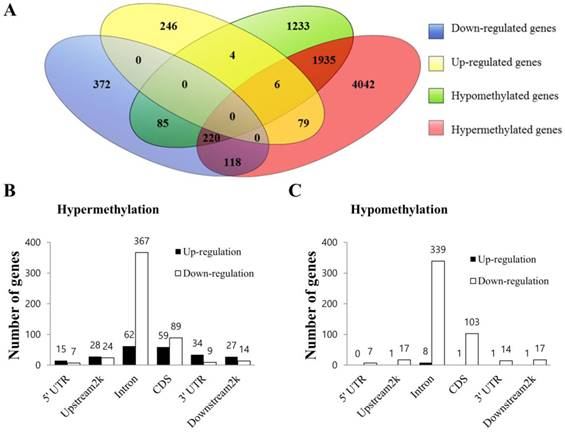
\includegraphics[width=0.8\textwidth]{journal-of-cancer_sample-result}}
	\caption{یک نمونه نمودار خلاصه برای نمایش نوآوری در نتایج
		%\cite{kim2016integrated}
	}
	\label{fig:sampleDiagram}
\end{figure}\\
طبیعتاً به صلاحدید نگارنده، شکل‌ها و نمودار‌ها می توانند در بخش های مختلف، خصوصا فصل
\ref{chap:results}
مورد استفاده قرار گیرند.

\subsection{تعریف واژه‌ها (اختیاری)}
در این قسمت محقق باید واژه‌هایی را که ممکن است برای خواننده آشنا نباشد، تعریف کند.

\subsection{خلاصه فصل‌ها}
در آخرین قسمتِ فصل اول پایان‌نامه، خلاصه‌ای اشاره‌وار از فصل‌های آتی آورده می‌شود تا خواننده بتواند تصویری واضح از دیگر قسمت‌های پایان‌نامه در ذهن خود ترسیم کند.

\section{جمع‌بندی}
در این فصل به دو مقولهٔ نحوه استفاده از قالب \پ دانشگاه تهران و نیز ویژگی‌هایی که محتویات فصل اول پایان‌نامه (یعنی مقدمه) باید داشته باشند، پرداخته شد. با توجه به اینکه این راهنما نحوه استفاده از قالب را شرح داده، ملزومات محتوایی هر فصل پایان‌نامه را توضیح می‌دهد و در پیوست‌ها نیز نحوهٔ کار با لاتک را یادآوری خواهد کرد، بنابراین مطالعهٔ کامل آن مقداری وقت شما را خواهد گرفت؛ اما مطمئن باشید از اتلاف وقت شما در ادامه کارتان تا حد زیادی جلوگیری خواهد کرد. در نوشتن متن حاضر سعی شده است علاوه بر ایجاد یک قالب لاتک برای پایان‌نامه‌های دانشگاه تهران، نکات محتوایی هر فصل نیز گوشزد گردد. طبیعتاً برای نگارش پایان‌نامهٔ خود می‌بایست مطالب تمام فصل‌ها را خودتان بازنویسی کنید.

در ادامهٔ این راهنما، تنها فصل‌هایی که یک پایان‌نامه باید داشته باشد و نیز خصوصیات یا ساختاری که محتویات هر فصل باید از آنها برخوردار باشد%
\footnote{از روی فایل «تمپلیت نگارش و تدوین پایان‌نامه \cite{UTThesisGuide}»}،
آورده می‌شوند. نهایتاً  در پیوست‌ها، مطالبی در باب یادآوری دستورات لاتک، نحوه نوشتن فرمول‌ها، تعاریف، قضایا، مثال‌ها، درج تصاویر، نمودارها، جداول و الگوریتم‌ها و نیز مدیریت مراجع، آمده است.

همچنین توصیه اکید دارم که رفع خطاهایی که احتمالاً با آنها مواجه می‌شوید را به آخر موکول نفرمایید و به محض برخورد با خطا، آن را اشکال‌زدایی و برطرف نمائید.!
و
\verb!% !TeX root=../main.tex
\setcounter{topnumber}{5}      % Increase number of floats at the top of the page
\setcounter{totalnumber}{5}    % Increase total number of floats on a page
\renewcommand{\floatpagefraction}{.8}  % Allow more of the page to be taken up by floats

\chapter{مروری بر مطالعات انجام شده}
%\thispagestyle{empty} 
\section{مقدمه}
در این فصل، پژوهش‌های پیشین در زمینه‌ی موتورهای مسطح مبتنی بر شناوری مغناطیسی (MLPM) با تمرکز بر ویژگی‌های اساسی آنان که به طور کلی در بخش‌های زیر دسته‌بندی شده‌اند، مورد بررسی قرار می‌گیرند. 
\begin{itemize}
	\item
		\textit{معماری دستگاه}:
بررسی انواع معماری‌های موجود برای MLPM و تأثیر آن‌ها بر عملکرد کلی سیستم.
	\item
		\textit{ساختار آهنرباهای دائمی و الکتریکی}:
مرور انواع آهنرباهای الکتریکی و چینش‌های مختلف آهنربا‌های دائمی و نقش آن‌ها در بهینه‌سازی عملکرد سیستم.
	\item
		\textit{طراحی کنترلر}:
معرفی روش‌های کنترل کلاسیک و مدرن برای این سیستم‌ها و چگونگی بهبود پایداری و دقت حرکت.
	\item
		\textit{روش‌های شناسایی سیستم و مدل‌سازی دینامیکی}:
تحلیل روش‌های شناسایی و تخمین مدل‌های دینامیکی سیستم برای شبیه‌سازی و بهینه‌سازی عملکرد.
\end{itemize}
در بخش‌های بعد، پژوهش‌های انجام‌شده بر اساس این ویژگی‌ها ارزیابی شده و مزایا و معایب هر روش مورد بررسی قرار می‌گیرد.

\section{معماری دستگاه‌های MLPM}
سیستم‌های شناوری مغناطیسی به دلیل ماهیت ناپایدارشان بدون استفاده از حلقه‌های کنترلی نمی‌توانند پایداری لازم را فراهم کنند. به همین دلیل، در تمامی ساختارهای پیشنهادی، از سیم‌پیچ‌های الکتریکی برای تولید میدان مغناطیسی با شدت کنترل ‌شده استفاده می‌شود. این سیم‌پیچ‌ها وظیفه دارند تا موقعیت جسم معلق را پایدار کرده و آن را در حالت مطلوب نگه ‌دارند.

در طراحی موتورهای مسطح، که از دو بخش ثابت
\LTRfootnote{Stator}
 و متحرک
\LTRfootnote{Mover}
تشکیل شده‌اند، امکان تغییر در طراحی و محل قرارگیری آهنرباهای الکتریکی و دائمی وجود دارد. نیروی مغناطیسی وارد بر بخش متحرک می‌تواند به‌صورت جاذبه‌ای از بالا یا دافعه‌ای از پایین اعمال شود. با این حال، در موتورهای مسطح به دلیل لزوم کم بودن فاصله میان سیم‌پیچ‌ها و اجسام معلق، اعمال نیروی جاذبه‌ای از بالا امکان‌پذیر نیست. به همین دلیل، در تمامی طراحی‌ها، نیروی مغناطیسی دافعه‌ای از سمت پایین به بخش متحرک وارد می‌شود که امکان جابه‌جایی اجسامی که بر روی آنها قرار می‌گیرند را فراهم می‌کند.

با توجه به این موارد، دو طراحی کلی برای ساخت دستگاه‌های MLPM ارائه می‌شود که در ادامه بررسی می‌‌شوند.
\subsection{سیم‌پیچ‌های متحرک و آهنرباهای ثابت}

در این معماری، بخش استاتور از مجموعه‌ای آهنربای ثابت تشکیل شده که میدان مغناطیسی پایدار در محیط اطراف خود ایجاد می‌کنند. بخش متحرک دستگاه شامل سیم‌پیچ‌هایی است که با عبور جریان الکتریکی از آن‌ها، میدان مغناطیسی متغیری تولید می‌گردد. این جریان به گونه‌ای تنظیم می‌شود که نیروی وارد بر آهنرباهای دائمی به‌دقت کنترل شود. طبق قانون سوم نیوتن، نیروهای وارد بر سیم‌پیچ‌ها و آهنرباهای دائمی به‌عنوان عمل و عکس‌العمل رفتار می‌کنند؛ به این ترتیب، نیرویی که به آهنرباها اعمال می‌شود، باعث ایجاد نیرویی برابر و در جهت مخالف بر سیم‌پیچ‌ها خواهد شد.

در پژوهش 
\cite{RN49}
، از ساختاری با سیم‌پیچ‌های چندلایه متعامد در بخش متحرک استفاده شده است. لایه اول سیم‌پیچ‌ها نیرویی را در راستاهای x و z ایجاد می‌کند، در حالی که لایه دوم نیرو را در راستاهای y و z اعمال می‌کند. این جداسازی نیروها به بهبود کنترل سیستم کمک می‌کند. علاوه بر این، به دلیل تفاوت فاصله میان لایه‌ها و استاتور، نیروهای تولیدشده توسط هر لایه متفاوت خواهند بود. راهکار ارائه‌شده برای این چالش، افزایش ضخامت لایه‌های دورتر از استاتور است. با این حال، برای جلوگیری از مشکلات ناشی از تفاوت ضخامت لایه‌ها، ساختاری سه‌لایه طراحی شده که ضمن افزایش نیروی تولیدی، ضخامت یکنواختی را در تمامی راستاها فراهم می‌نماید. در شکل 
\ref{fig:Multilayer_Mover_Coil}
ساختار این دستگاه نمایش داده شده است.

در پژوهش 
\cite{RN38}
، بخش متحرک از یک لایه سیم‌پیچ با چینش متعامد تشکیل شده که قابلیت اعمال نیرو در سه راستا را فراهم می‌سازد. در ادامه، پژوهش
\cite{RN14}
 روشی تحلیلی برای بهینه‌سازی ضخامت این سیم‌پیچ‌ها ارائه کرده است که با در نظر گرفتن معیارهای مختلف، به بهبود عملکرد سیستم می‌پردازد. شکل 
\ref{fig:Single_layer_Mover_Coil}
 این ساختار را نمایش داده است.

\begin{figure}[ht]
\centering 
\subfloat[استفاده از سیم‌پیچ‌های چندلایه
\cite{RN49}]
{ \label{fig:Multilayer_Mover_Coil}
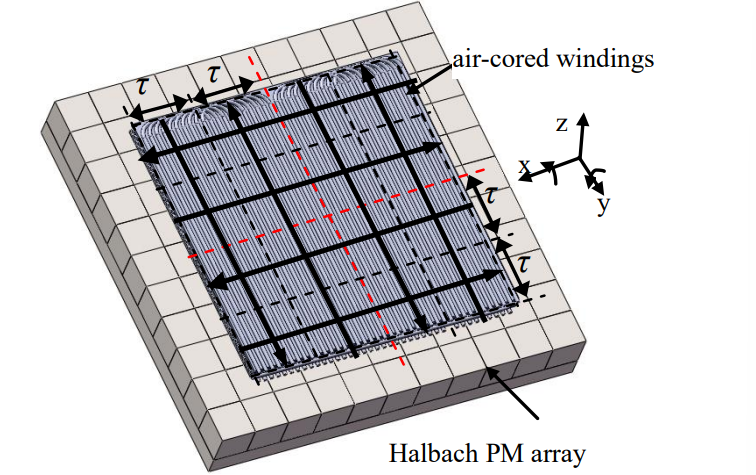
\includegraphics[width=0.5\textwidth]{Multilayer_Mover_Coil}}
%\hspace{2mm}
\subfloat[استفاده از سیم‌پیچ‌های یک لایه متعامد
\cite{RN14}]
{ \label{fig:Single_layer_Mover_Coil}
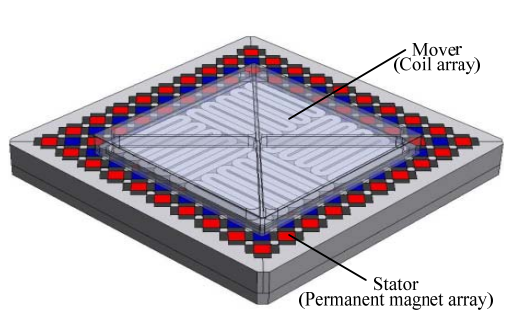
\includegraphics[width=0.5\textwidth]{Single_layer_Mover_Coil}}%
\caption{ساختار سیستم‌های MLPM با سیم‌پیچ‌های متحرک و آهنربای ثابت}
\label{fig:Moveing_Coil} %% label for entire figure
\end{figure}

با وجود اینکه این معماری امکان دستیابی به شناوری پایدار و حرکت با شش درجه آزادی را فراهم می‌کند، اما در کاربردهای عملی با محدودیت‌هایی مواجه است که بر عملکرد نهایی سیستم تأثیرگذار هستند. نخستین محدودیت، نیاز به تأمین انرژی الکتریکی برای سیم‌پیچ‌ها از طریق سیم‌های فیزیکی است که این امر به‌طور اجتناب‌ناپذیری ارتباط فیزیکی میان جسم متحرک و محیط اطراف را برقرار می‌سازد، در نتیجه حرکت آزادانه کامل جسم متحرک محدود می‌شود. دومین محدودیت، چالش خنک‌کاری سیم‌پیچ‌ها است که به دلیل ماهیت متحرک و معلق بودن آن‌ها، اجرای یک سیستم خنک‌کننده کارآمد دشوار خواهد بود. این مشکلات، نیاز به ارائه معماری جدیدی را آشکار می‌کند که بتواند این چالش‌ها را برطرف سازد.

\subsection{‌آهنرباهای متحرک و سیم‌پیچ‌های ثابت}

معماری دیگری که برای طراحی دستگاه‌های MLPM ارائه شده است، شامل قرار دادن سیم‌پیچ‌ها در بخش استاتور و استفاده از آهنرباهای دائمی در بخش متحرک می‌باشد. این ساختار نوین که در بسیاری از پژوهش‌ها مورد استفاده قرار گرفته، مشکلات معماری‌های پیشین مانند محدودیت جابه‌جایی متحرک ناشی از اتصالات فیزیکی و چالش‌های خنک‌کاری سیم‌پیچ‌ها را برطرف کرده و منجر به بهبود عملکرد کلی سیستم شده است.

در پژوهش 
\cite{RN7}
 استاتوری با چینش سیم‌پیچ‌ها مطابق با الگوی شاه‌ماهی
\LTRfootnote{Herringbone pattern}
 طراحی و پیاده‌سازی شده است. این طراحی امکان اعمال نیروی مغناطیسی به دو آهنربای دیسکی تعبیه‌شده در بخش متحرک را فراهم کرده است که دقتی در حدود 1 درجه در زوایای حرکت و 1 میلی‌متر در موقعیت متحرک به دست آورده است
\cite{RN7}
. در ادامه این پژوهش، ساختاری جدید برای بخش متحرک ارائه شده که شامل 6 آهنربای دیسکی با چینش کروی و فواصل ثابت می‌باشد. این طراحی توانسته است چرخش آزادانه متحرک را حول سه محور ممکن سازد 
\cite{RN39}.
شکل (
\ref{fig:Moving_Magnet_1})
همچنین در پژوهش 
\cite{RN62}
 نیز از این چینش سیم‌پیچ‌ها استفاده شده و مطابق با شبیه‌سازی‌های ارائه شده، مزیت آنان در ایجاد میدان مغناطیسی یکنواخت‌تر در نواحی کناری سیم‌پیچ‌ها نمایش داده شده است.

استفاده از سیم‌پیچ‌های سه‌فاز به‌جای تغذیه با جریان مستقیم، رویکردی است که در پژوهش 
\cite{RN24}
معرفی و اجرا شده است. در این ساختار، چهار آرایه از سیم‌پیچ‌های سه‌فاز، همان‌طور که در 
شکل (
\ref{fig:Moving_Magnet_2})
 نشان داده شده است، به‌گونه‌ای طراحی شده‌اند که نیروی مغناطیسی لازم را تولید کنند.

به ‌منظور کاهش هزینه‌ی محاسباتی در جابه‌جایی‌های طولانی، پژوهش 
\cite{RN32}
 ساختاری را ارائه کرده است که از دو مجموعه سیم‌پیچ‌ سه‌فاز و تک‌فاز تشکیل شده است. در این طراحی، کنترل حرکت در مسافت‌های طولانی توسط سیم‌پیچ‌های سه‌فاز انجام می‌پذیرد، در حالی که برای تنظیم دقیق موقعیت متحرک در صفحه، از سیم‌پیچ‌های تک‌فاز بهره برده می‌شود.
شکل (
\ref{fig:Moving_Magnet_3})

استفاده از سیم‌پیچ‌های ماژولار در طراحی استاتورهایی با چینش دوبعدی، رویکردی است که در دستگاه‌های MagTable و MagFloor از دانشگاه واترلو پیاده‌سازی شده است
\cite{RN8,RN30,RN10}
 در این طراحی، ماژول‌هایی از سیم‌پیچ‌های با سطح مقطع مربع به‌گونه‌ای طراحی شده‌اند که با قرار گرفتن در کنار یکدیگر، فضای کاری نامحدودی برای جابه‌جایی متحرک فراهم می‌کنند.(شکل
\ref{fig:Moving_Magnet_4})
 همچنین، پژوهش
\cite{RN8}
 نشان داده است که آهنرباهای با سطح مقطع مربع، در مقایسه با سیم‌پیچ‌های دایروی با جریان الکتریکی مشابه، می‌توانند شدت میدان مغناطیسی بیشتری ایجاد کنند، که این مزیت عملکرد کلی سیستم را بهبود می‌بخشد.

\begin{figure}[ht]
\centering 
\subfloat[الگوی شاه‌ماهی سیم‌پیچ‌ها
\cite{RN39}]
{ \label{fig:Moving_Magnet_1}
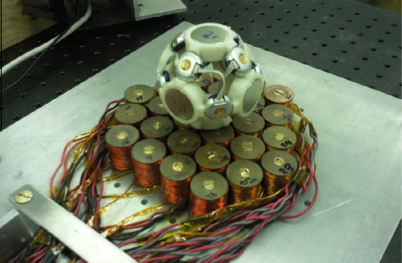
\includegraphics[width=0.45\textwidth]{Moving_Magnet_1}}
\hspace{2mm}
\subfloat[سیم‌پیچ‌های سه فاز
\cite{RN24}]
{ \label{fig:Moving_Magnet_2}
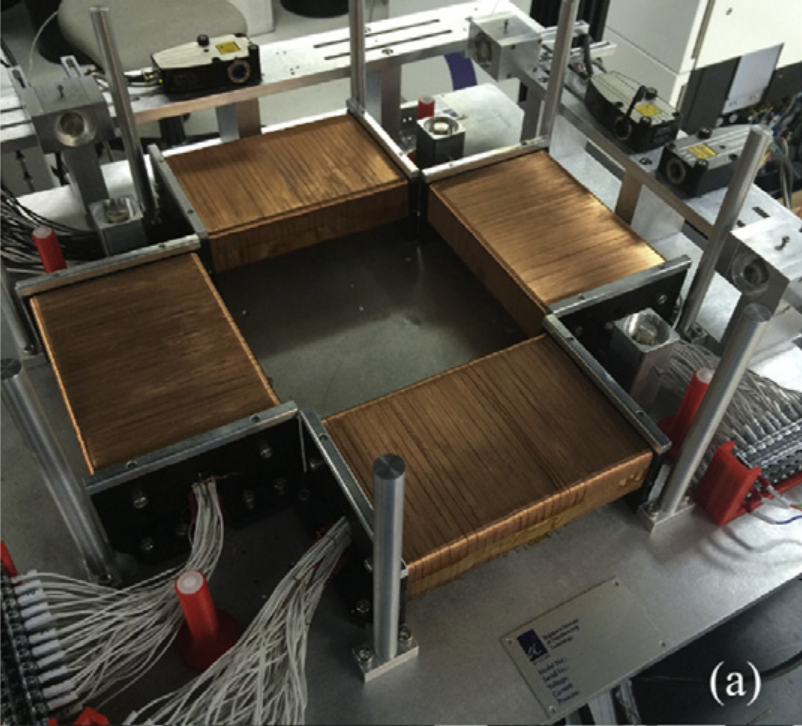
\includegraphics[width=0.45\textwidth]{Moving_Magnet_2}}
\\ % Newline to wrap the figures to the next row
\subfloat[ساختار دوگانه سیم‌پیچ‌ها
\cite{RN32}]
{ \label{fig:Moving_Magnet_3}
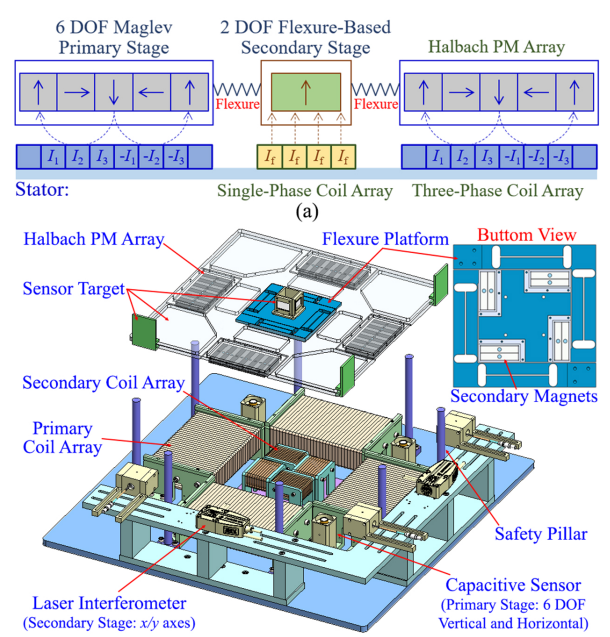
\includegraphics[width=0.45\textwidth]{Moving_Magnet_3}}
\hspace{2mm}
\subfloat[ساختار ماژولار سیم‌پیچ‌ها
\cite{RN10}]
{ \label{fig:Moving_Magnet_4}
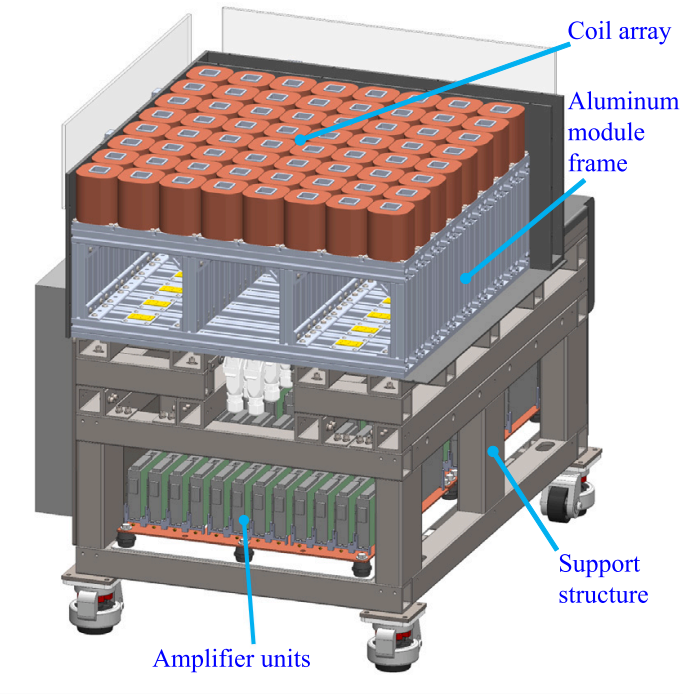
\includegraphics[width=0.45\textwidth]{Moving_Magnet_4}}
\label{fig:Moveing_Magnet} %% label for entire figure
\caption{ساختارهای آهنرباهای متحرک و سیم‌پیچ‌های ثابت}
\end{figure}








\section{ساختار آهنرباهای دائمی}

همان‌طور که در بخش قبل اشاره شد، میدان مغناطیسی کنترل‌شده توسط آهنرباهای الکتریکی ایجاد می‌شود و بر اثر تعامل این میدان متغیر با میدان ثابت آهنرباهای دائمی، نیرویی بر بخش متحرک دستگاه وارد می‌شود که حرکت آن را در راستاهای مختلف ممکن می‌سازد. بنابراین، طراحی بهینه آهنرباهای دائمی، به‌ویژه برای تولید میدان مغناطیسی قوی‌تر با کمترین وزن، در بهبود کارایی دستگاه نقش کلیدی دارد. در این بخش، طراحی‌های مختلف آهنرباهای دائمی که در پژوهش‌های پیشین ارائه شده‌اند، با تمرکز بر بهینه‌سازی این ویژگی‌ها بررسی می‌شوند.
\subsection{استفاده از آهنرباهای دیسکی}

استفاده از آهنرباهای دیسکی رویکردی ساده و مؤثر برای ایجاد میدان مغناطیسی دائمی محسوب می‌شود. با انتخاب موادی با خاصیت مغناطیسی بالا، مانند آهنرباهای نئودیمیومی، می‌توان به شدت میدان مغناطیسی مطلوب دست یافت. به عنوان نمونه، در پژوهش 
\cite{RN7}
 از دو آهنربای دیسکی جهت تأمین میدان مغناطیسی ثابت استفاده شده است. همچنین در پژوهش 
\cite{RN39}
 با به‌کارگیری ۶ آهنربای دیسکی، امکان چرخش آزادانه حول سه محور فراهم شده است.(شکل
\ref{fig:Disk_Magnet_1})
 در پژوهش 
\cite{RN8}
 نیز از ترکیب‌های متفاوتی از آهنرباهای دیسکی برای بخش متحرک دستگاه استفاده شده است، که این ترکیب‌ها شامل تغییر اندازه‌ی یک آهنربا و استفاده از سه آهنربای دیسکی است. سیستم شناوری مغناطیسی با پنج درجه آزادی که تنها از یک آهنربای دیسکی تشکیل شده است، در پژوهش 
\cite{RN62}
 به عنوان نمونه‌ای موفق از این رویکرد معرفی شده است. این طراحی، با وجود سادگی معماری، توانسته نتایج رضایت‌بخشی را از نظر عملکرد ارائه دهد و نشان می‌دهد که استفاده از آهنربای دیسکی، علاوه بر سادگی، می‌تواند در کاربردهای مختلف به‌ویژه در سیستم‌های با نیاز به دقت بالا و چند درجه آزادی، کارآمد باشد. شکل((
\ref{fig:Disk_Magnet_2})


\begin{figure}[ht]
\centering 
\subfloat[دو آهنربای دیسکی
\cite{RN7}]
{ \label{fig:Disk_Magnet_1}
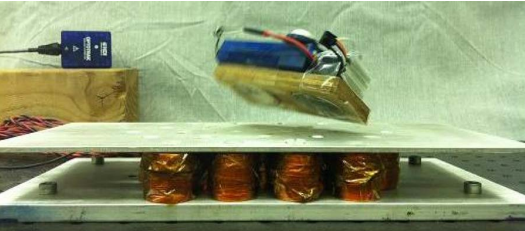
\includegraphics[width=0.5\textwidth]{Disk_Magnet_1}}
%\hspace{2mm}
\subfloat[یک آهنربای دیسکی
\cite{RN62}]
{ \label{fig:Disk_Magnet_2}
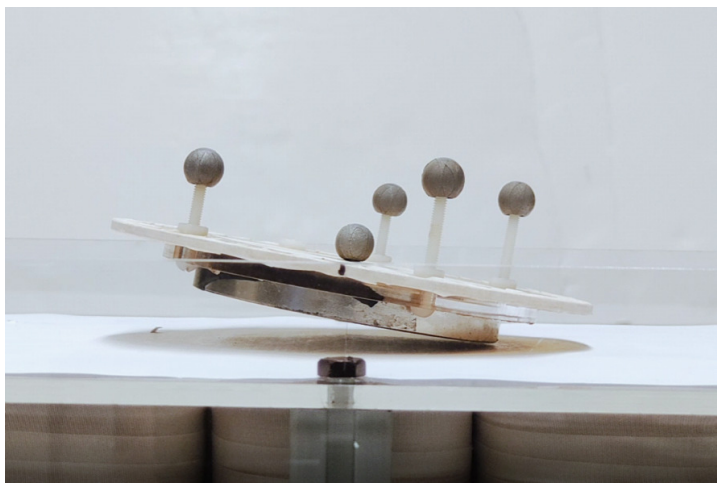
\includegraphics[width=0.5\textwidth]{Disk_Magnet_2}}%
\caption{استفاده از آهنربای دیسکی در طراحی متحرک}
\label{fig:Disk_Magnet} %% label for entire figure
\end{figure}



\subsection{آرایه‌ی هالباخ یک بعدی}

آرایه‌ی هالباخ
\LTRfootnote{Halbach Array}
 به‌عنوان چینشی از آهنرباهای دائمی تعریف می‌شود که در آن جهت مغناطیس‌شوندگی هر آهنربا با آهنربای مجاور خود ۹۰ درجه تفاوت دارد. این آرایه به‌طور خاص قادر است میدان مغناطیسی در یک سوی آرایه را خنثی کرده و در سوی دیگر میدان را به میزان تقریبی 1.4 برابر افزایش دهد.
مزیت این ساختار در طراحی سیستم‌های MLPM، توانایی آن در تولید شدت میدان مغناطیسی بیشتر است. به‌همین‌دلیل، این چینش در بسیاری از پژوهش‌ها مورد استفاده قرار گرفته است.
با این حال، استفاده از تنها یک آرایه‌ی یک‌بعدی هالباخ به‌تنهایی نمی‌تواند نیرویی در دو راستای افقی ایجاد کند. لذا معمولاً از تعداد بیشتری از این آرایه‌ها در ساختار متحرک استفاده می‌شود. به‌عنوان مثال، در پژوهش‌های 
\cite{RN24,RN27}
 از چهار آرایه‌ی هالباخ یک‌بعدی در بخش متحرک استفاده شده است که هر یک از این آرایه‌ها قادر به ایجاد نیرویی در یکی از راستاهای افقی و عمودی هستند.
در پژوهش 
\cite{RN39}
، مشابه آنچه که در بخش استاتور پیاده‌سازی شده بود، از ساختار دوگانه‌ای در بخش متحرک بهره‌برداری شده است، به‌گونه‌ای که دو مجموعه چهارگانه از آرایه‌های هالباخ در معماری این بخش به‌کار رفته‌اند.

\begin{figure}[ht]
\centering 
\subfloat[آرایه‌ی هالباخ
\cite{RN16}]
{ \label{fig:halbach1D}
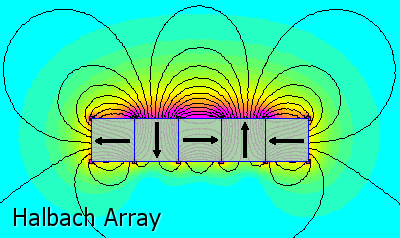
\includegraphics[width=0.5\textwidth]{halbach1D}}
%\hspace{2mm}
\subfloat[4 آرایه‌ی یک بعدی هالباخ
\cite{RN39}]
{ \label{fig:4_halbach1D_array}
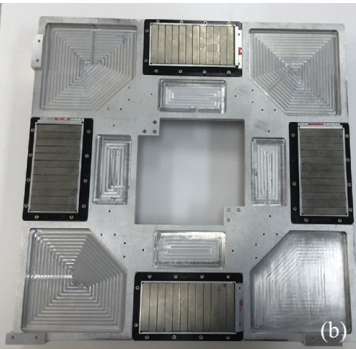
\includegraphics[width=0.5\textwidth]{4_halbach1D_array}}%
\caption{آرایه هالباخ یک‌بعدی}
\label{fig:halbach1D} %% label for entire figure
\end{figure}

\subsection{آرایه هالباخ دوبعدی}

برای رفع محدودیت‌های آرایه‌ی هالباخ یک‌بعدی که تنها در یک راستا نیرو ایجاد می‌کند، ساختار جدیدی از آرایه‌ی دوبعدی ارائه شده است. این آرایه قادر است میدان مغناطیسی را در یک طرف صفحه حذف و در طرف دیگر تقویت کند. با این ویژگی، استفاده از چندین آرایه برای تأمین میدان مغناطیسی ثابت ضروری نخواهد بود. طراحی آرایه‌ی دوبعدی در بسیاری از پژوهش‌ها برای بخش‌های متحرک یا استاتور سیستم‌های MLPM به کار گرفته شده است.

استفاده از آرایه‌ی هالباخ در پژوهش‌های مختلفی از جمله
\cite{RN10, RN30} 
و
\cite{RN55, RN26} 
نشان‌دهنده‌ی عملکرد بهینه‌ی این معماری در بخش متحرک سیستم‌های MLPM است.(شکل
\ref{fig:halbach2D_2})
 همچنین در پژوهش
\cite{RN14}
 از این آرایه به عنوان بخشی از استاتور دستگاه بهره‌گیری شده است. در 
\cite{RN61}
 ماژول‌هایی برای ساخت این آرایه استفاده شده (شکل
\ref{fig:halbach2D_4})
 و در
\cite{RN49}
 برای تشکیل آرایه از قطعات آهنی در فضای خالی میان آن استفاده شده است؛ اما این رویکرد باعث ایجاد خطا در دقت میدان مغناطیسی شده است. (شکل
\ref{fig:halbach2D_3})
علاوه بر این، در پژوهش
\cite{RN28}
، طراحی جدیدی با آهنرباهایی با میزان مغناطیس‌شوندگی و ارتفاع متفاوت پیشنهاد شده است.
\begin{figure}[ht]
\centering 
\subfloat[آرایه هالباخ دو بعدی و میدان مغناطیسی آن
\cite{RN10}]
{ \label{fig:halbach2D_2}
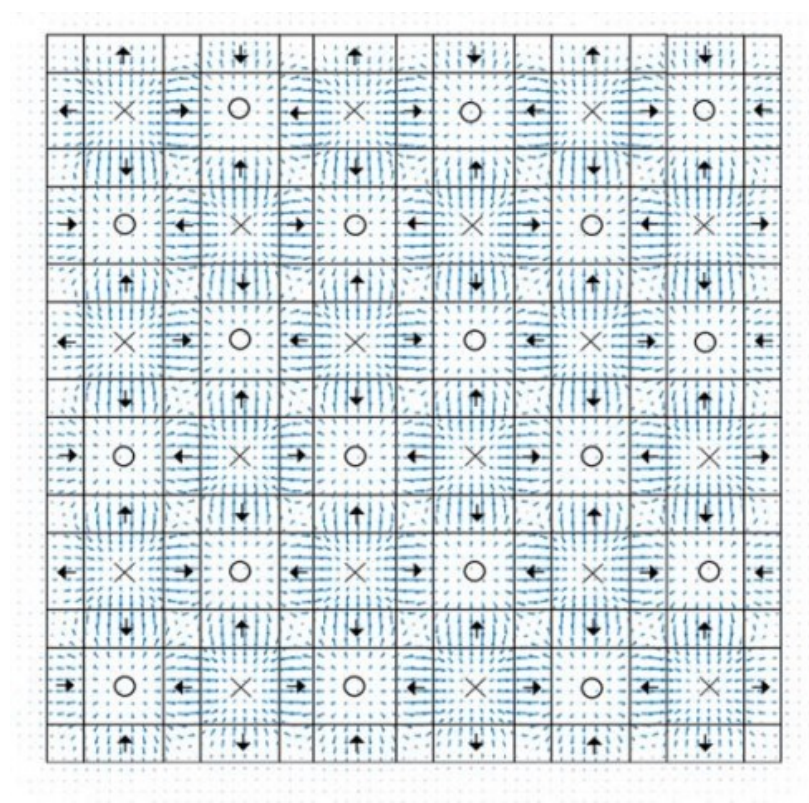
\includegraphics[width=0.45\textwidth]{halbach2D_2}}
\hspace{2mm}
\subfloat[آرایه هالباخ دوبعدی با قطعات آهنی در فضاهای خالی
\cite{RN49}]
{ \label{fig:halbach2D_3}
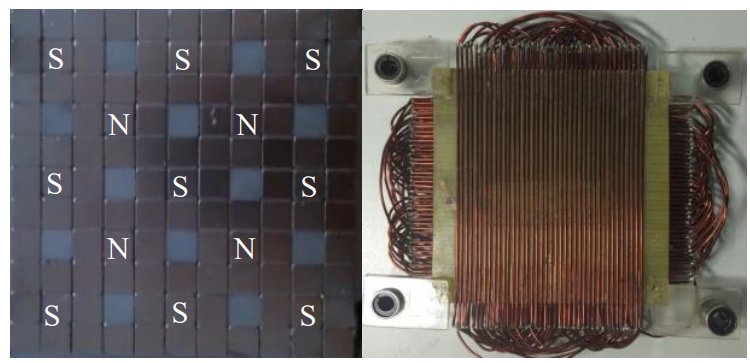
\includegraphics[width=0.45\textwidth]{halbach2D_3}}
\\ % Newline to wrap the figures to the next row
\subfloat[آرایه هالباخ دوبعدی ماژولار
\cite{RN61}]
{ \label{fig:halbach2D_4}
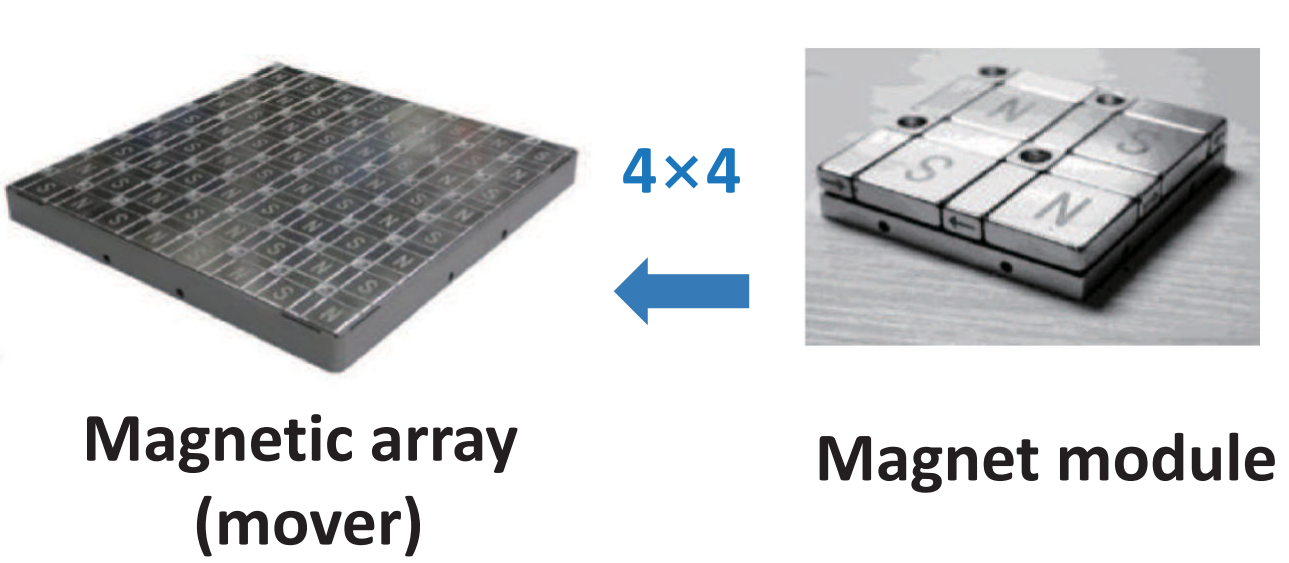
\includegraphics[width=0.45\textwidth]{halbach2D_4}}
\caption{آرایه هالباخ دو‌بعدی}
\label{fig:halbach2D} %% label for entire figure

\end{figure}
\section{طراحی کنترلر}
همان‌طور که پیش‌تر اشاره شد، سیستم‌های شناوری مغناطیسی ذاتاً ناپایدار هستند و برای دستیابی به پایداری، به کنترلری با عملکرد دقیق و خطای کم نیاز است. در پژوهش‌های مختلف، از کنترلرهای گوناگونی برای این سیستم‌ها بهره گرفته شده است؛ از جمله کنترلرهای کلاسیک نظیر PID، کنترلرهای مدرن مانند کنترل مبتنی بر پیش‌بینی مدل (MPC) و همچنین مدل‌های مبتنی بر هوش مصنوعی نظیر شبکه‌های بازگشتی GRU. در این بخش، به بررسی این کنترلرها و مقایسه‌ عملکرد آنها خواهیم پرداخت.
\subsection{کنترلر PID}

کنترل تناسبی-انتگرالی-مشتقی (PID) به عنوان یکی از پرکاربردترین و موثرترین کنترلرهای کلاسیک در سیستم‌های دینامیکی، گزینه‌ای مناسب برای کنترل سیستم‌های MLPM محسوب می‌شود. این کنترلر به دلیل سادگی در پیاده‌سازی، تنظیم دقیق و توانایی تنظیم خروجی سیستم بر اساس خطاهای ورودی، به‌طور گسترده در سیستم‌های مختلف استفاده شده است. برای کنترل سیستم‌های MLPM، به ازای هر درجه آزادی یک کنترلر PID طراحی و پیاده‌سازی می‌شود تا بتواند جریان الکتریکی سیم‌پیچ‌ها را تنظیم کرده و میدان مغناطیسی لازم برای ایجاد و حفظ موقعیت متحرک را تأمین کند.

در پژوهش‌های متعددی از کنترلر PID برای سیستم‌های MLPM بهره گرفته شده است. به عنوان مثال، در 
\cite{RN39,RN24}
از کنترلرهای PID ساده برای کنترل جریان سیم‌پیچ‌ها استفاده شده که وظیفه تنظیم میدان مغناطیسی و در نتیجه، کنترل موقعیت جسم متحرک را بر عهده دارند. علاوه بر این، در پژوهش
\cite{RN32}
، از دو کنترلر PID در یک ساختار دوگانه استفاده شده است. کنترلر اول برای جابه‌جایی‌های بلند و در مسافت‌های طولانی به کار رفته و جریان سیم‌پیچ‌های اصلی را تنظیم می‌کند، در حالی که کنترلر دوم برای حرکات دقیق کوتاه‌برد طراحی شده و کنترل جریان سیم‌پیچ‌های ثانویه را بر عهده دارد. این روش باعث بهینه‌سازی کنترل دقیق و بهبود دقت در حرکات کوتاه‌برد و جابه‌جایی‌های سریع می‌شود.
همچنین در سیستم MagTable، برای کنترل دقیق موقعیت آهنرباهای دائمی، از شش کنترلر PID به‌صورت همزمان استفاده شده است تا نیروی متوازن برای پایدارسازی موقعیت متحرک در چندین جهت فراهم شود 
\cite{RN8}
. این نوع طراحی و استفاده از کنترلرهای PID نشان می‌دهد که علی‌رغم محدودیت‌های موجود در کنترلرهای کلاسیک، این روش همچنان در بسیاری از سیستم‌های مغناطیسی پیچیده مانند MLPM کارایی بالایی دارد.

\begin{figure}[ht]
\centering{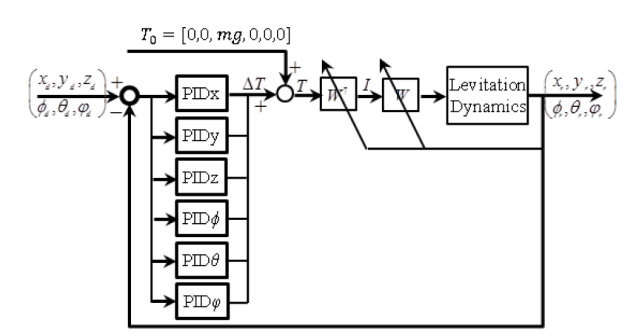
\includegraphics[width=0.5\textwidth]{PID_1}}
\caption{کنترلر PID با 6 درجه آزادی
\cite{RN8}}
\label{fig:PID}
\end{figure}


\subsection{کنترلر مبتنی بر پیش‌بینی مدل MPC}
برای کنترل سیستم‌های MLPM اگر مدل سیستم به روش‌های تحلیلی و یا عددی به دست آمده و تخمین زده شده باشد، می‌توان از این مدل‌ها برای طراحی کنترلرهای پیشرفته‌تر با هدف پیش‌بینی رفتار سیستم و استفاده از آن به صورت پیش‌خور در حلقه‌ی کنترلی استفاده کرد. روش‌های تخمین مدل این سیستم‌ها در بخش‌های بعد مورد بررسی قرار می‌گیرد. در این بخش، کنترلرهای ارائه شده در پژوهش‌های دیگر ارائه می‌شود.
به دست آوردن معادلات دینامیکی سیستم و استفاده از آنها در پیش‌بینی روشی تحلیلی است که در 
\cite{RN55}
 استفاده شده است و مدل کنترلی متشکل از بلوک‌های پس‌خور و پیش‌خور برای کنترل موقعیت آهنربا طراحی شده است. همچنین در 
\cite{RN62}
 از یک جدول جستجو برای تعیین رفتار سیستم در نقاط مختلف فضا استفاده شده است که این جدول به عنوان پیش‌خور به مدل کنترلی داده می‌شود. در ادامه‌ی این پژوهش، با استفاده از روش‌های شناسایی سیستم، مدلی تقریبی برای رفتار سیستم در نظر گرفته شده است و با استفاده از این مدل برای پیش‌بینی رفتار سیستم‌ مدل MPC پیاده‌سازی شده است. پژوهش 
\cite{RN30}
 با تمرکز بر ارائه‌ی یک مدل پیش‌بین، با استفاده از معادلات دینامیکی سیستم و همچنین روش‌پیش‌بینی حالت بی‌تاخیر، رفتار آینده‌ی سیستم را محاسبه می‌کند.
\begin{figure}[ht]
\centering 
\subfloat[\cite{RN55}]{
    \label{fig:MPC_1}
    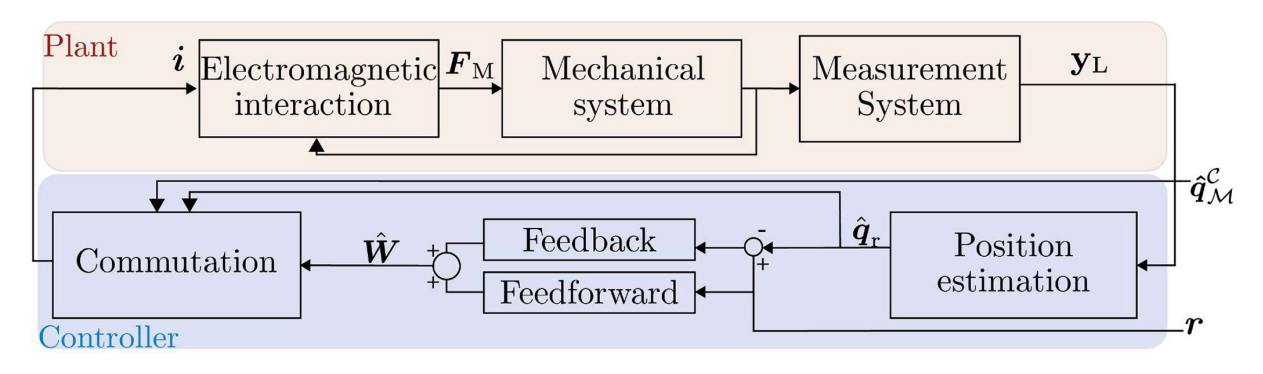
\includegraphics[width=0.45\textwidth]{MPC_1}}
%\hspace{2mm}
\subfloat[\cite{RN62}]{
    \label{fig:MPC_2}
    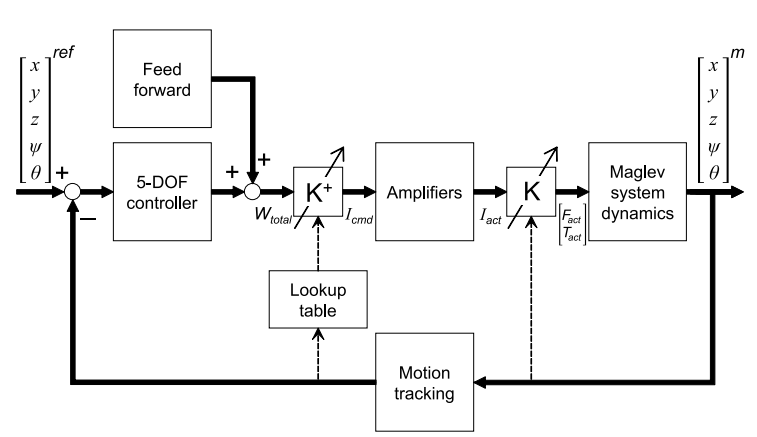
\includegraphics[width=0.45\textwidth]{MPC_2}}
\\ % Newline to wrap the figures to the next row
\subfloat[\cite{RN61}]{
    \label{fig:MPC_3}
    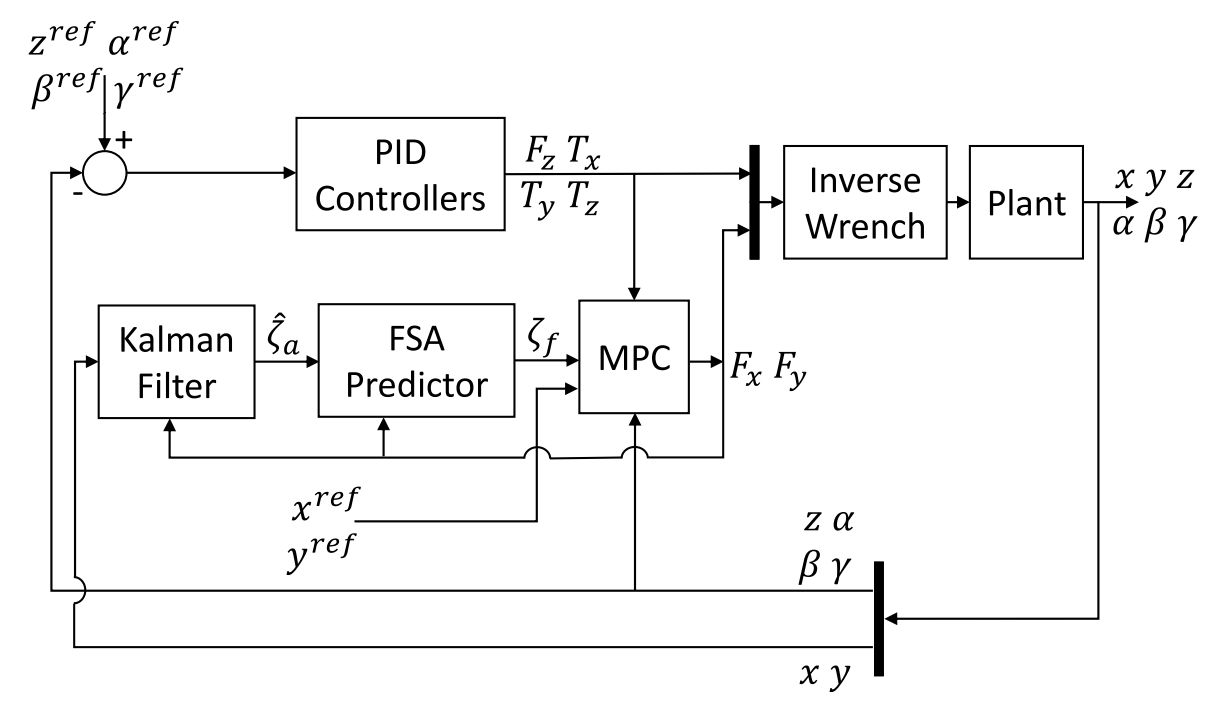
\includegraphics[width=0.45\textwidth]{MPC_3}}
\subfloat[\cite{RN61}]{
    \label{fig:MPC_4}
    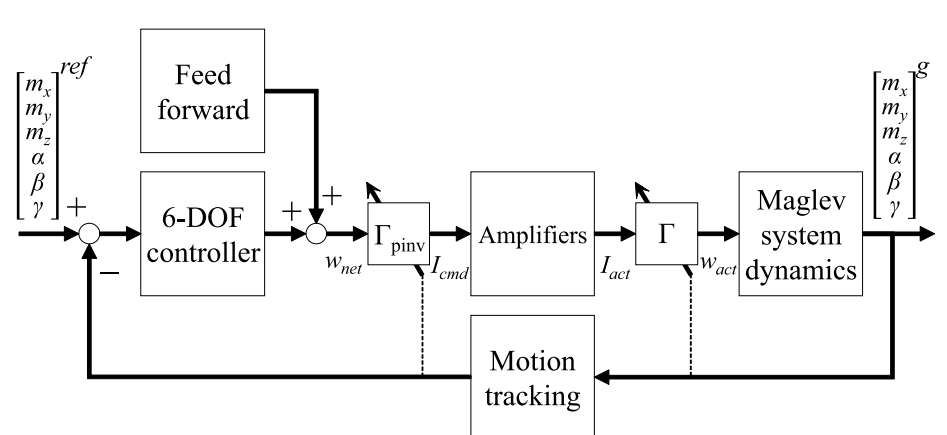
\includegraphics[width=0.45\textwidth]{MPC_4}}
\caption{کنترلر MPC}
\label{fig:MPC} %% label for entire figure
\end{figure}

\FloatBarrier

\subsection{کنترلر مبتنی بر هوش مصنوعی}

یکی از روش‌های نوین برای پیش‌بینی رفتار سیستم‌های پیچیده مانند MLPM، استفاده از مدل‌های هوش مصنوعی به‌ویژه شبکه‌های عصبی بازگشتی (RNN) است. این مدل‌ها با یادگیری دینامیک سیستم و ارتباط بین ورودی‌ها و خروجی‌ها، می‌توانند به‌طور مؤثری رفتار سیستم را در شرایط مختلف پیش‌بینی کنند. در این راستا، پژوهش
\cite{RN61}
از یک مدل بازگشتی GRU 
\LTRfootnote{Gated Recurrent Unit}
 استفاده کرده است. این مدل بر اساس داده‌های جمع‌آوری‌شده از عملکرد دستگاه MLPM آموزش دیده و توانسته است با دقت بالا تغییرات دینامیکی سیستم و پاسخ آن به ورودی‌های گوناگون را پیش‌بینی کند. استفاده از GRU به دلیل توانایی آن در مدل‌سازی وابستگی‌های زمانی و در نظر گرفتن اطلاعات قبلی برای پیش‌بینی‌های دقیق‌تر، رویکردی مناسب در این پژوهش بوده است.(شکل 
\ref{fig:GRU}

\begin{figure}[ht]
\centering
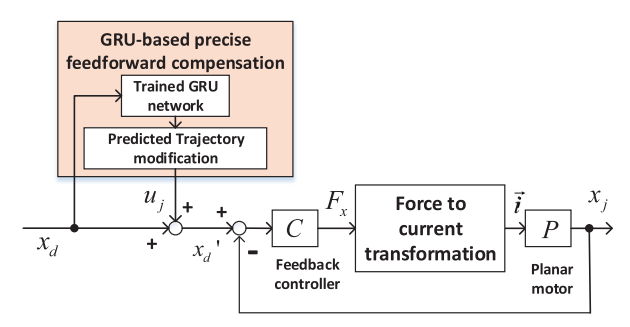
\includegraphics[width=0.5\textwidth]{GRU_1}
\caption{کنترلر پیش‌خور GRU \cite{RN61}}
\label{fig:GRU}
\end{figure}

\section{مدل‌سازی و تخمین سیستم}
در روش بار نقطه‌ای برای تحلیل میدان مغناطیسی، فرض می‌شود که توزیع بار مغناطیسی در یک حجم به‌صورت متمرکز در هشت نقطه در گوشه‌های آن حجم قرار گرفته است. با این فرض، اثر مغناطیسی این جسم می‌تواند به‌صورت مجموع آثار هر یک از بارهای نقطه‌ای محاسبه شود. این رویکرد امکان محاسبه‌ی دقیق شدت میدان مغناطیسی و نیروی وارد بر یک جسم خارجی را فراهم می‌آورد. از طریق محاسبه‌ی میدان‌های ناشی از هر بار نقطه‌ای و جمع آنها، میدان مغناطیسی کل حاصل می‌شود و به این ترتیب، شدت میدان مغناطیسی ناشی از آهنربای دائمی به کمک این روش به‌طور دقیق محاسبه می‌گردد. در ادامه، معادلات مربوط به محاسبه‌ی شدت میدان مغناطیسی ارائه شده‌اند.
\subsection{مدل بار مغناطیسی سطحی}
در این مدل، فرض بر این است که بار مغناطیسی در یک المان حجم سه‌بعدی به‌صورت توزیعی از بارهای مغناطیسی با چگالی بار J بر روی دو صفحه‌ی موازی قرار گرفته است. با استفاده از این فرض، میدان مغناطیسی ایجادشده توسط این حجم به‌صورت میدان حاصل از توزیع بارهای مغناطیسی محاسبه می‌شود. این مدل امکان تحلیل دقیق‌تر رفتار میدان مغناطیسی را فراهم می‌کند. مقایسه نتایج حاصل از این مدل با شبیه‌سازی المان محدود
\LTRfootnote{Finite Element Method (FEM)}
 در پژوهش
\cite{RN44}
نشان داده است که این روش مدل‌سازی برای سیستم‌های MLPM دقت و کارایی بالایی دارد.

\begin{figure}[ht]
\centering
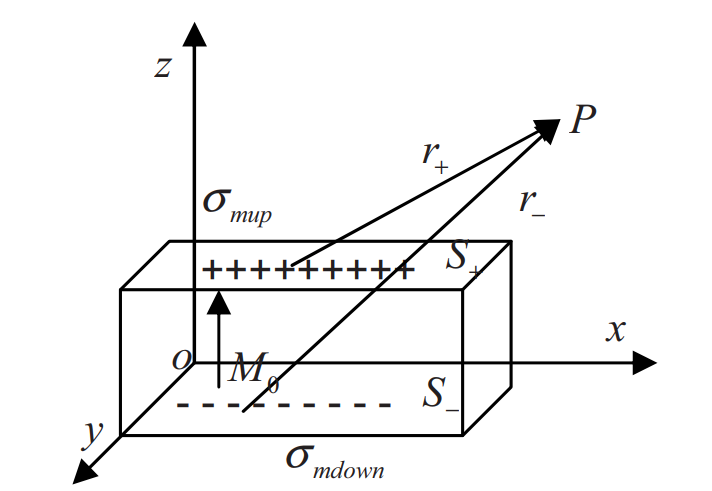
\includegraphics[width=0.5\textwidth]{Magnetic surface charge_2}
\caption{مدل بار مغناطیسی سطحی \cite{RN44}}
\label{fig:Magnetic surface charge}
\end{figure}

\subsection{مدل بار مغناطیسی نقطه‌ای}
در روش بار نقطه‌ای برای تحلیل میدان مغناطیسی، فرض می‌شود که توزیع بار مغناطیسی در یک حجم به‌صورت متمرکز در هشت نقطه در گوشه‌های آن حجم قرار گرفته است. با این فرض، اثر مغناطیسی این جسم می‌تواند به‌صورت مجموع آثار هر یک از بارهای نقطه‌ای محاسبه شود. این رویکرد امکان محاسبه‌ی دقیق شدت میدان مغناطیسی و نیروی وارد بر یک جسم خارجی را فراهم می‌آورد. از طریق محاسبه‌ی میدان‌های ناشی از هر بار نقطه‌ای و جمع آنها، میدان مغناطیسی کل حاصل می‌شود و به این ترتیب، شدت میدان مغناطیسی ناشی از آهنربای دائمی به کمک این روش به‌طور دقیق محاسبه می‌گردد. در ادامه، معادلات مربوط به محاسبه‌ی شدت میدان مغناطیسی ناشی از هر بار نقطه‌ای ارائه شده‌است.
\begin{align}
B_{xk} &= \frac{\epsilon_k}{4\pi} \ln\left(-y_r + \sqrt{x_r^2 + y_r^2 + z_r^2}\right), \\
B_{yk} &= \frac{\epsilon_k}{4\pi} \ln\left(-x_r + \sqrt{x_r^2 + y_r^2 + z_r^2}\right), \\
B_{zk} &= \frac{\epsilon_k}{4\pi} \arctan\left( \frac{x_r y_r}{\sqrt{x_r^2 + y_r^2 + z_r^2}} \right),
\end{align}

\begin{figure}[ht]
\centering
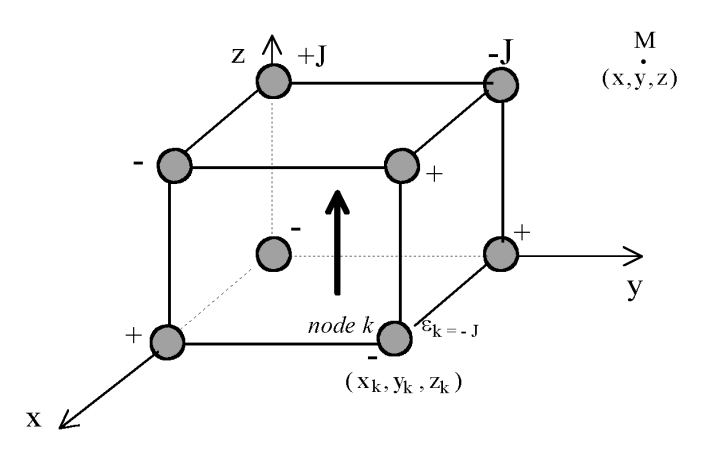
\includegraphics[width=0.5\textwidth]{Magnetic_Node}
\caption{مدل بار مغناطیسی نقطه‌ای \cite{RN44}}
\label{figMagnetic_Node}
\end{figure}

\subsection{مدل های مبتنی بر داده}

در این روش‌ها، به‌جای مدل‌سازی دقیق ساختار فیزیکی دستگاه و استخراج معادلات دینامیکی آن، پارامترهای مورد نیاز مانند شدت میدان مغناطیسی از طریق داده‌های تجربی یا شبیه‌سازی المان محدود (FEM) تخمین زده می‌شوند. این رویکرد مبتنی بر داده نیازمند دسترسی به اطلاعات دقیق از سیستم واقعی یا شبیه‌سازی کامل آن است تا بتوان دقت و اعتبار تخمین‌ها را ارزیابی کرد. در پژوهش 
\cite{RN10}
، برای تخمین شدت میدان مغناطیسی آرایه هالباخ دوبعدی از معادلات هارمونیک و سری فوریه استفاده شده است. تغییرات میدان مغناطیسی تولیدشده توسط این آرایه به‌صورت موجی سینوسی مدل‌سازی شده است، اما این روش تنها زمانی دقیق است که فرض شود سطح آرایه به‌صورت نامحدود ادامه دارد. برای حل این مشکل، آرایه به سه ناحیه مرکزی، کناری و گوشه‌ای تقسیم‌بندی شده و برای هر ناحیه هارمونیک‌های مجزا در نظر گرفته شده است. نتایج این پژوهش نشان می‌دهند که با استفاده از سه هارمونیک اول، می‌توان میدان مغناطیسی را در نواحی کناری و گوشه‌ای با دقت مناسبی تخمین زد.

\begin{figure}[ht]
\centering 
\subfloat[\cite{RN10}]{
\label{fig:harmonic_1}
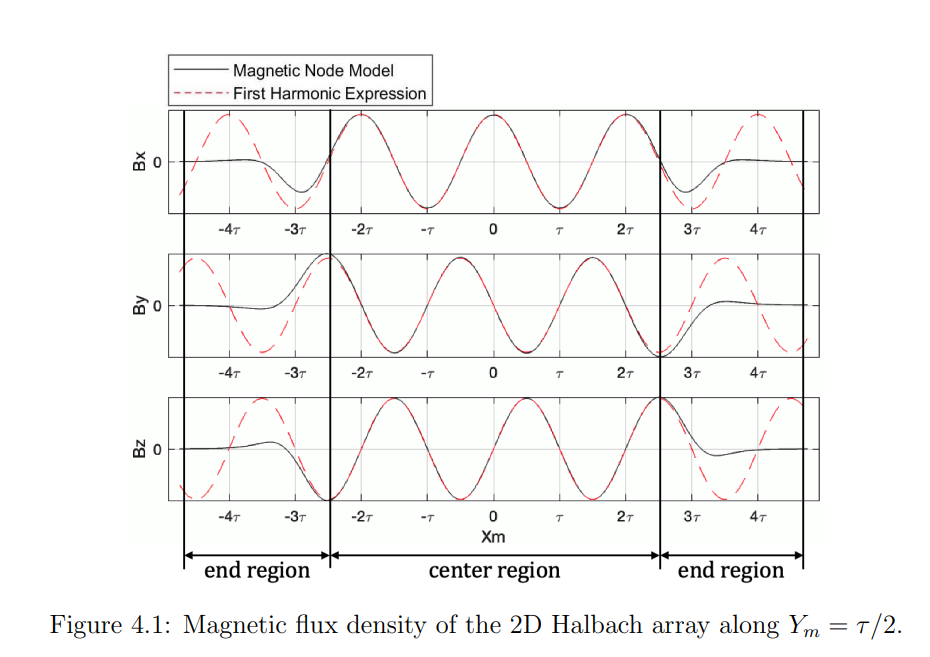
\includegraphics[width=0.45\textwidth]{harmonic_1}}
\hspace{2mm}
\subfloat[\cite{RN10}]{
\label{fig:harmonic_2}
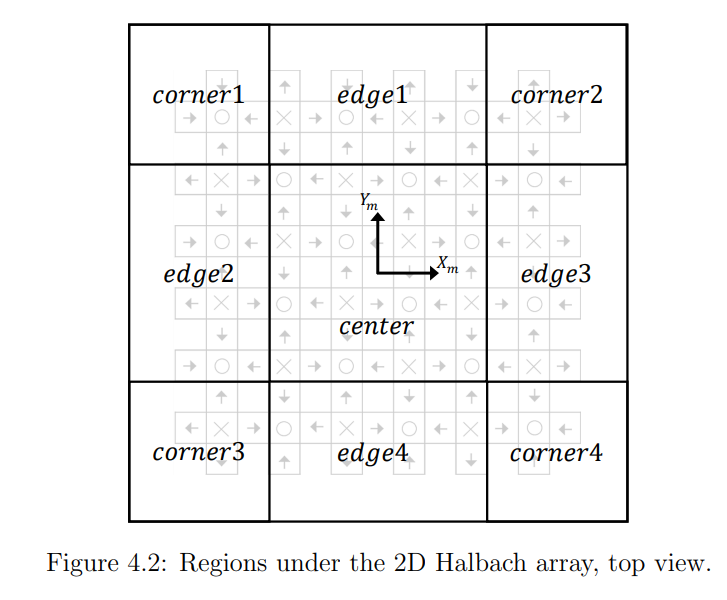
\includegraphics[width=0.45\textwidth]{harmonic_2}}
\caption{مدل هارمونیک}
\label{fig:harmonic}
\end{figure}



!
را در فایل 
\lr{main.tex}،
غیرفعال%
\footnote{
برای غیرفعال کردن یک دستور، کافی است در ابتدای آن، علامت درصد انگلیسی (\%) بگذارید.
}
 کنید. در غیر این صورت، ابتدا مطالب دو فصل اول پردازش شده و سپس مطالب فصل ۳ پردازش می‌شود که این کار باعث طولانی شدن زمان پردازش می‌گردد. هر زمان که خروجی کل \پ را خواستید، تمام فصل‌ها را دوباره در
\lr{main.tex}
فعال نمائید.
بدیهتاً لازم نیست فصل‌های \پ را به ترتیب تایپ کنید. مثلاً می‌توانید ابتدا مطالب فصل ۳ را تایپ نموده و سپس مطالب فصل ۱ را تایپ کنید. 
\subsubsection{مراجع}
برای وارد کردن مراجع \پ کافی است فایل 
\lr{MyReferences.bib}
را باز کرده و مراجع خود را به شکل اقلام نمونهٔ داخل آن، وارد کنید.  سپس از \lr{bibtex} برای تولید مراجع با قالب مناسب استفاده نمائید. برای توضیحات بیشتر بخش \ref{Sec:Ref} از پیوست \ref{app:latexIntro} و نیز پیوست \ref{app:refMan} را ببینید.

\subsubsection{واژه‌نامه فارسی به انگلیسی و برعکس}
برای وارد کردن معادل فارسی اصطلاحات لاتین در متن و تهیه فهرست واژه‌نامه از آنها، از بستهٔ
\lr{glossaries}
و نرم‌افزار
\lr{xindy}
استفاده می‌شود. بدین منظور کافی است اصطلاحات لاتین و ترجمهٔ آنها را در فایل
\lr{words.tex}
وارد کرده و هر جای متن که خواستید با دستورات
\verb|gls{label}|
یا \verb|glspl{label}|
معادل فارسی مفرد یا جمع یک اصطلاح را بیاورید.

مثلا در اینجا، واژهٔ
«\gls{Action}»
برای بار اول و دوباره
«\gls{Action}»
برای بار دوم در متن ظاهر شده است.
جهت توضیحات بیشتر به پیوست
\ref{app:refMan}
مراجعه کنید.
\subsubsection{نمایه}
برای وارد کردن نمایه، باید از 
\lr{xindy}
استفاده کنید. 
%زیرا 
%\lr{MakeIndex}
%با حروف «گ»، «چ»، «پ»، «ژ» و «ک» مشکل دارد و ترتیب الفبایی این حروف را رعایت نمی‌کند. همچنین، فاصله بین هر گروه از کلمات در 
%\lr{MakeIndex}،
%به درستی رعایت نمی‌شود که باعث زشت شدن حروف‌چینی این قسمت می‌شود. 
راهنمای چگونگی کار با 
\lr{xindy} 
را می‌توانید در ویکی پارسی‌لاتک و یا مثالهای موجود در دی‌وی‌دی «مجموعه پارسی‌لاتک»، پیدا کنید.

\subsection{اگر سوالی داشتم، از کی بپرسم؟}
برای پرسیدن سوال‌های خود موقع حروف‌چینی با زی‌پرشین، می‌توانید به
\href{http://qa.parsilatex.com}{سایت پرسش و پاسخ پارسی‌لاتک}%
\LTRfootnote{http://qa.parsilatex.com}
یا
\href{http://forum.parsilatex.com}{بایگانی تالارگفتگوی قدیمی پارسی‌لاتک}%
\LTRfootnote{http://forum.parsilatex.com}
مراجعه کنید. شما هم می‌توانید روزی به سوال‌های دیگران در اینترنت جواب دهید.
بستهٔ زی‌پرشین و بسیاری از بسته‌های مرتبط با آن مانند
\lr{bidi} و
\lr{Persian-bib}،
مجموعه پارسی‌لاتک، مثالهای مختلف موجود در آن، قالب پایان‌نامه دانشگاههای مختلف و سایت پارسی‌لاتک همه به صورت داوطلبانه توسط افراد گروه پارسی‌لاتک و گروه
\lr{Persian TeX}
و بدون هیچ کمک مالی انجام شده‌اند. کار اصلی نوشتن و توسعه زی‌پرشین توسط آقای وفا خلیقی انجام شده است که این کار بزرگ را به انجام رساندند.
اگر مایل به کمک به گروه پارسی‌لاتک هستید به سایت این گروه مراجعه فرمایید:
\begin{center}
	\url{http://www.parsilatex.com}
\end{center}

\section{محتویات فصل اول یک پایان‌نامه}
فصل اول یک پایان‌نامه باید به مقدمه یا کلیات تحقیق بپردازد.
هدف از فصل مقدمه%
\LTRfootnote{Introduction}،
شرح مختصر مسأله تحقیق، اهمیت و انگیزه محقق از پرداختن به آن موضوع، بهمراه اشاره‌ای کوتاه به روش و مراحل تحقیق است. مقدمه، اولین فصل از ساختار اصلی \پ بوده و زمینه اطلاعاتی لازم را برای خواننده فراهم می‌آورد. در طول مقدمه باید سعی شود موضوع تحقیق با زبانی روشن، ساده و بطور عمیق و هدفمند به خواننده معرفی شود. این فصل باید خواننده را مجذوب و اهمیت موضوع تحقیق را آشکار سازد. در مقدمه باید با ارائهٔ سوابق، شواهد تحقیقی و اطلاعات موجود (با ذکر منبع) با روشی منظم، منطقی و هدف‌دار، خواننده را جهت داد و به سوی راه حل مورد نظر هدایت کرد. مقدمه مناسب‌ترین جا برای ارائهٔ اختصارات و بعضی توضیحات کلی است، توضیحاتی که شاید نتوان در مباحث دیگر آنها را شرح داد.

مقدمه، یکی از ارکان اساسی و اصلی پایان نامه است که مهمترین قسمت‌های آن عبارتند از: 

\subsection{عنوان تحقیق} 
باید شناختی دقیق و روشن از حوزهٔ موضوع تحقیق را عرضه دارد و خالی از هرگونه ابهام و پیچیدگی باشد.

\subsection{مسأله تحقیق}
وظیفه اصلی مقدمه بیان این مطلب به خواننده است که چرا انجام تحقیق را به عهده گرفته‌اید. اگر دلیل شما برای انجام این کار پاسخگویی به سؤال مورد علاقه‌تان است، با مشکل زیادی روبه‌رو نخواهید بود. یکی از بهترین روش‌ها برای نوشتن مقدمهٔ یک پایان‌نامه، طرح پرسش یا پرسش‌هایی مهم و اساسی است که کار تحقیقاتی شما از آغاز تا پایان قصد پاسخ دادن به آن را دارد. گاهی می‌توانید ابتدا اهمیت موضوع را بیان و سپس پرسش خود را در آن موضوع مطرح کنید.

\subsection{تاریخچه‌ای از موضوع تحقیق}
به طور کلی تشریح روندهای تحقیقاتی در محدودهٔ مورد مطالعه، مستلزم ارجاع به کارهای دیگران است. بعضی از نویسندگان برای کارهای دیگران هیچ اعتباری قائل نمی‌شوند و در مقابل، بعضی دیگر از نویسندگان در توصیف کارهای دیگران، بسیار زیاده‌روی می‌کنند. اکثر مواقع، ارجاع به مقالات دو سال قبل از کارتان، بهتر از نوشتن سطرهای مرجع است. در این قسمت باید به طور مختصر به نظرات و تحقیقات مربوط به موضوع و یا مسائل و مشکلات حل نشده در این حوزه و همچنین توجه و علاقه جامعه به این موضوع، اشاره شود.

\subsection{تعریف موضوع تحقیق}
در این قسمت محقق، موضوع مورد علاقه و یا نیاز احساس شدهٔ خود را در حوزه تحقیق بیان می‌دارد و عوامل موجود در موقعیت را تعریف و تعیین می‌کند.

\subsection{هدف یا هدف‌های کلی و آرمانی تحقیق}
این قسمت باید با جملات مثبت و کلی طرح شود و از طولانی شدن مطالب پرهیز شود.

\subsection{روش انجام تحقیق}
در این قسمت، پژوهشگر روش کاری خود را بیان می‌دارد و شیوه‌های گوناگونی را که در گردآوری مطالب خود بکار برده، ذکر می‌کند. همچنین اگر روش آماری خاصی را در تهیه و تدوین اطلاعات به کار برده است، آن شیوه را نیز اینجا بیان می‌کند.

\subsection{نوآوری، اهمیت و ارزش تحقیق}
در این قسمت، در مورد نوآوری علمی و عملی تحقیق که محقق به آن دست خواهد یافت، بحث می‌شود. ممکن است لازم باشد تا برخی نمودارهای خلاصه در این بخش استفاده شوند. به عنوان مثال، نموداری از مقاله
\cite{kim2016integrated}
در شکل
\ref{fig:sampleDiagram}
آمده است.
\begin{figure}[ht]
	\centerline{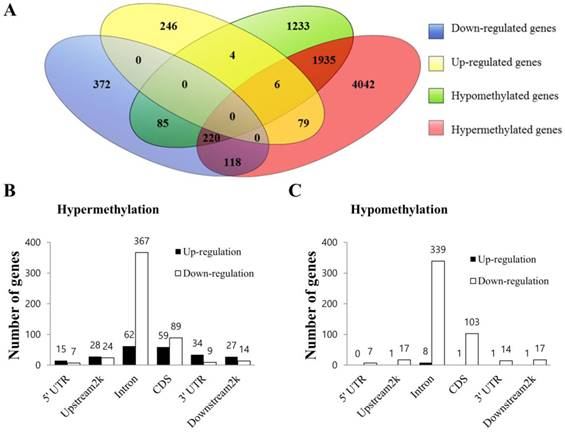
\includegraphics[width=0.8\textwidth]{journal-of-cancer_sample-result}}
	\caption{یک نمونه نمودار خلاصه برای نمایش نوآوری در نتایج
		%\cite{kim2016integrated}
	}
	\label{fig:sampleDiagram}
\end{figure}\\
طبیعتاً به صلاحدید نگارنده، شکل‌ها و نمودار‌ها می توانند در بخش های مختلف، خصوصا فصل
\ref{chap:results}
مورد استفاده قرار گیرند.

\subsection{تعریف واژه‌ها (اختیاری)}
در این قسمت محقق باید واژه‌هایی را که ممکن است برای خواننده آشنا نباشد، تعریف کند.

\subsection{خلاصه فصل‌ها}
در آخرین قسمتِ فصل اول پایان‌نامه، خلاصه‌ای اشاره‌وار از فصل‌های آتی آورده می‌شود تا خواننده بتواند تصویری واضح از دیگر قسمت‌های پایان‌نامه در ذهن خود ترسیم کند.

\section{جمع‌بندی}
در این فصل به دو مقولهٔ نحوه استفاده از قالب \پ دانشگاه تهران و نیز ویژگی‌هایی که محتویات فصل اول پایان‌نامه (یعنی مقدمه) باید داشته باشند، پرداخته شد. با توجه به اینکه این راهنما نحوه استفاده از قالب را شرح داده، ملزومات محتوایی هر فصل پایان‌نامه را توضیح می‌دهد و در پیوست‌ها نیز نحوهٔ کار با لاتک را یادآوری خواهد کرد، بنابراین مطالعهٔ کامل آن مقداری وقت شما را خواهد گرفت؛ اما مطمئن باشید از اتلاف وقت شما در ادامه کارتان تا حد زیادی جلوگیری خواهد کرد. در نوشتن متن حاضر سعی شده است علاوه بر ایجاد یک قالب لاتک برای پایان‌نامه‌های دانشگاه تهران، نکات محتوایی هر فصل نیز گوشزد گردد. طبیعتاً برای نگارش پایان‌نامهٔ خود می‌بایست مطالب تمام فصل‌ها را خودتان بازنویسی کنید.

در ادامهٔ این راهنما، تنها فصل‌هایی که یک پایان‌نامه باید داشته باشد و نیز خصوصیات یا ساختاری که محتویات هر فصل باید از آنها برخوردار باشد%
\footnote{از روی فایل «تمپلیت نگارش و تدوین پایان‌نامه \cite{UTThesisGuide}»}،
آورده می‌شوند. نهایتاً  در پیوست‌ها، مطالبی در باب یادآوری دستورات لاتک، نحوه نوشتن فرمول‌ها، تعاریف، قضایا، مثال‌ها، درج تصاویر، نمودارها، جداول و الگوریتم‌ها و نیز مدیریت مراجع، آمده است.

همچنین توصیه اکید دارم که رفع خطاهایی که احتمالاً با آنها مواجه می‌شوید را به آخر موکول نفرمایید و به محض برخورد با خطا، آن را اشکال‌زدایی و برطرف نمائید.!
و
\verb!% !TeX root=../main.tex
\setcounter{topnumber}{5}      % Increase number of floats at the top of the page
\setcounter{totalnumber}{5}    % Increase total number of floats on a page
\renewcommand{\floatpagefraction}{.8}  % Allow more of the page to be taken up by floats

\chapter{مروری بر مطالعات انجام شده}
%\thispagestyle{empty} 
\section{مقدمه}
در این فصل، پژوهش‌های پیشین در زمینه‌ی موتورهای مسطح مبتنی بر شناوری مغناطیسی (MLPM) با تمرکز بر ویژگی‌های اساسی آنان که به طور کلی در بخش‌های زیر دسته‌بندی شده‌اند، مورد بررسی قرار می‌گیرند. 
\begin{itemize}
	\item
		\textit{معماری دستگاه}:
بررسی انواع معماری‌های موجود برای MLPM و تأثیر آن‌ها بر عملکرد کلی سیستم.
	\item
		\textit{ساختار آهنرباهای دائمی و الکتریکی}:
مرور انواع آهنرباهای الکتریکی و چینش‌های مختلف آهنربا‌های دائمی و نقش آن‌ها در بهینه‌سازی عملکرد سیستم.
	\item
		\textit{طراحی کنترلر}:
معرفی روش‌های کنترل کلاسیک و مدرن برای این سیستم‌ها و چگونگی بهبود پایداری و دقت حرکت.
	\item
		\textit{روش‌های شناسایی سیستم و مدل‌سازی دینامیکی}:
تحلیل روش‌های شناسایی و تخمین مدل‌های دینامیکی سیستم برای شبیه‌سازی و بهینه‌سازی عملکرد.
\end{itemize}
در بخش‌های بعد، پژوهش‌های انجام‌شده بر اساس این ویژگی‌ها ارزیابی شده و مزایا و معایب هر روش مورد بررسی قرار می‌گیرد.

\section{معماری دستگاه‌های MLPM}
سیستم‌های شناوری مغناطیسی به دلیل ماهیت ناپایدارشان بدون استفاده از حلقه‌های کنترلی نمی‌توانند پایداری لازم را فراهم کنند. به همین دلیل، در تمامی ساختارهای پیشنهادی، از سیم‌پیچ‌های الکتریکی برای تولید میدان مغناطیسی با شدت کنترل ‌شده استفاده می‌شود. این سیم‌پیچ‌ها وظیفه دارند تا موقعیت جسم معلق را پایدار کرده و آن را در حالت مطلوب نگه ‌دارند.

در طراحی موتورهای مسطح، که از دو بخش ثابت
\LTRfootnote{Stator}
 و متحرک
\LTRfootnote{Mover}
تشکیل شده‌اند، امکان تغییر در طراحی و محل قرارگیری آهنرباهای الکتریکی و دائمی وجود دارد. نیروی مغناطیسی وارد بر بخش متحرک می‌تواند به‌صورت جاذبه‌ای از بالا یا دافعه‌ای از پایین اعمال شود. با این حال، در موتورهای مسطح به دلیل لزوم کم بودن فاصله میان سیم‌پیچ‌ها و اجسام معلق، اعمال نیروی جاذبه‌ای از بالا امکان‌پذیر نیست. به همین دلیل، در تمامی طراحی‌ها، نیروی مغناطیسی دافعه‌ای از سمت پایین به بخش متحرک وارد می‌شود که امکان جابه‌جایی اجسامی که بر روی آنها قرار می‌گیرند را فراهم می‌کند.

با توجه به این موارد، دو طراحی کلی برای ساخت دستگاه‌های MLPM ارائه می‌شود که در ادامه بررسی می‌‌شوند.
\subsection{سیم‌پیچ‌های متحرک و آهنرباهای ثابت}

در این معماری، بخش استاتور از مجموعه‌ای آهنربای ثابت تشکیل شده که میدان مغناطیسی پایدار در محیط اطراف خود ایجاد می‌کنند. بخش متحرک دستگاه شامل سیم‌پیچ‌هایی است که با عبور جریان الکتریکی از آن‌ها، میدان مغناطیسی متغیری تولید می‌گردد. این جریان به گونه‌ای تنظیم می‌شود که نیروی وارد بر آهنرباهای دائمی به‌دقت کنترل شود. طبق قانون سوم نیوتن، نیروهای وارد بر سیم‌پیچ‌ها و آهنرباهای دائمی به‌عنوان عمل و عکس‌العمل رفتار می‌کنند؛ به این ترتیب، نیرویی که به آهنرباها اعمال می‌شود، باعث ایجاد نیرویی برابر و در جهت مخالف بر سیم‌پیچ‌ها خواهد شد.

در پژوهش 
\cite{RN49}
، از ساختاری با سیم‌پیچ‌های چندلایه متعامد در بخش متحرک استفاده شده است. لایه اول سیم‌پیچ‌ها نیرویی را در راستاهای x و z ایجاد می‌کند، در حالی که لایه دوم نیرو را در راستاهای y و z اعمال می‌کند. این جداسازی نیروها به بهبود کنترل سیستم کمک می‌کند. علاوه بر این، به دلیل تفاوت فاصله میان لایه‌ها و استاتور، نیروهای تولیدشده توسط هر لایه متفاوت خواهند بود. راهکار ارائه‌شده برای این چالش، افزایش ضخامت لایه‌های دورتر از استاتور است. با این حال، برای جلوگیری از مشکلات ناشی از تفاوت ضخامت لایه‌ها، ساختاری سه‌لایه طراحی شده که ضمن افزایش نیروی تولیدی، ضخامت یکنواختی را در تمامی راستاها فراهم می‌نماید. در شکل 
\ref{fig:Multilayer_Mover_Coil}
ساختار این دستگاه نمایش داده شده است.

در پژوهش 
\cite{RN38}
، بخش متحرک از یک لایه سیم‌پیچ با چینش متعامد تشکیل شده که قابلیت اعمال نیرو در سه راستا را فراهم می‌سازد. در ادامه، پژوهش
\cite{RN14}
 روشی تحلیلی برای بهینه‌سازی ضخامت این سیم‌پیچ‌ها ارائه کرده است که با در نظر گرفتن معیارهای مختلف، به بهبود عملکرد سیستم می‌پردازد. شکل 
\ref{fig:Single_layer_Mover_Coil}
 این ساختار را نمایش داده است.

\begin{figure}[ht]
\centering 
\subfloat[استفاده از سیم‌پیچ‌های چندلایه
\cite{RN49}]
{ \label{fig:Multilayer_Mover_Coil}
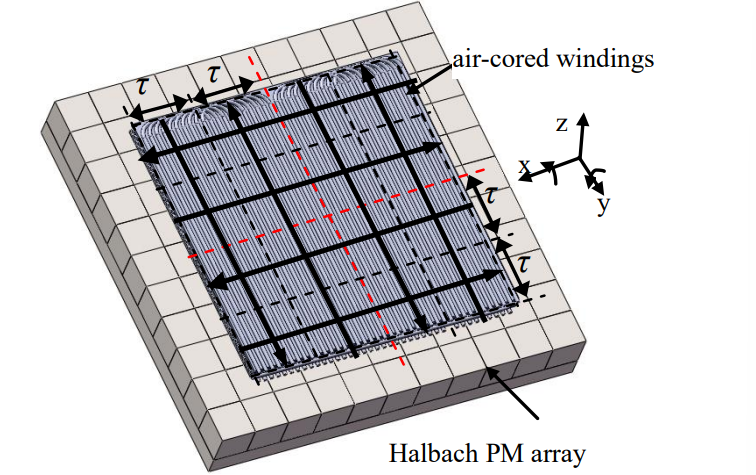
\includegraphics[width=0.5\textwidth]{Multilayer_Mover_Coil}}
%\hspace{2mm}
\subfloat[استفاده از سیم‌پیچ‌های یک لایه متعامد
\cite{RN14}]
{ \label{fig:Single_layer_Mover_Coil}
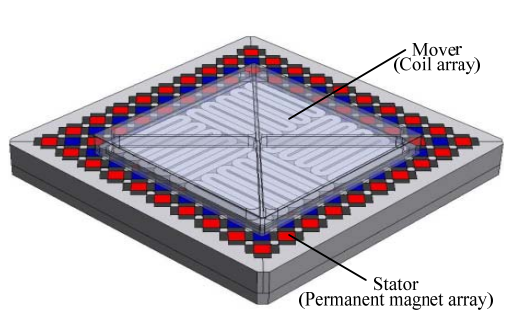
\includegraphics[width=0.5\textwidth]{Single_layer_Mover_Coil}}%
\caption{ساختار سیستم‌های MLPM با سیم‌پیچ‌های متحرک و آهنربای ثابت}
\label{fig:Moveing_Coil} %% label for entire figure
\end{figure}

با وجود اینکه این معماری امکان دستیابی به شناوری پایدار و حرکت با شش درجه آزادی را فراهم می‌کند، اما در کاربردهای عملی با محدودیت‌هایی مواجه است که بر عملکرد نهایی سیستم تأثیرگذار هستند. نخستین محدودیت، نیاز به تأمین انرژی الکتریکی برای سیم‌پیچ‌ها از طریق سیم‌های فیزیکی است که این امر به‌طور اجتناب‌ناپذیری ارتباط فیزیکی میان جسم متحرک و محیط اطراف را برقرار می‌سازد، در نتیجه حرکت آزادانه کامل جسم متحرک محدود می‌شود. دومین محدودیت، چالش خنک‌کاری سیم‌پیچ‌ها است که به دلیل ماهیت متحرک و معلق بودن آن‌ها، اجرای یک سیستم خنک‌کننده کارآمد دشوار خواهد بود. این مشکلات، نیاز به ارائه معماری جدیدی را آشکار می‌کند که بتواند این چالش‌ها را برطرف سازد.

\subsection{‌آهنرباهای متحرک و سیم‌پیچ‌های ثابت}

معماری دیگری که برای طراحی دستگاه‌های MLPM ارائه شده است، شامل قرار دادن سیم‌پیچ‌ها در بخش استاتور و استفاده از آهنرباهای دائمی در بخش متحرک می‌باشد. این ساختار نوین که در بسیاری از پژوهش‌ها مورد استفاده قرار گرفته، مشکلات معماری‌های پیشین مانند محدودیت جابه‌جایی متحرک ناشی از اتصالات فیزیکی و چالش‌های خنک‌کاری سیم‌پیچ‌ها را برطرف کرده و منجر به بهبود عملکرد کلی سیستم شده است.

در پژوهش 
\cite{RN7}
 استاتوری با چینش سیم‌پیچ‌ها مطابق با الگوی شاه‌ماهی
\LTRfootnote{Herringbone pattern}
 طراحی و پیاده‌سازی شده است. این طراحی امکان اعمال نیروی مغناطیسی به دو آهنربای دیسکی تعبیه‌شده در بخش متحرک را فراهم کرده است که دقتی در حدود 1 درجه در زوایای حرکت و 1 میلی‌متر در موقعیت متحرک به دست آورده است
\cite{RN7}
. در ادامه این پژوهش، ساختاری جدید برای بخش متحرک ارائه شده که شامل 6 آهنربای دیسکی با چینش کروی و فواصل ثابت می‌باشد. این طراحی توانسته است چرخش آزادانه متحرک را حول سه محور ممکن سازد 
\cite{RN39}.
شکل (
\ref{fig:Moving_Magnet_1})
همچنین در پژوهش 
\cite{RN62}
 نیز از این چینش سیم‌پیچ‌ها استفاده شده و مطابق با شبیه‌سازی‌های ارائه شده، مزیت آنان در ایجاد میدان مغناطیسی یکنواخت‌تر در نواحی کناری سیم‌پیچ‌ها نمایش داده شده است.

استفاده از سیم‌پیچ‌های سه‌فاز به‌جای تغذیه با جریان مستقیم، رویکردی است که در پژوهش 
\cite{RN24}
معرفی و اجرا شده است. در این ساختار، چهار آرایه از سیم‌پیچ‌های سه‌فاز، همان‌طور که در 
شکل (
\ref{fig:Moving_Magnet_2})
 نشان داده شده است، به‌گونه‌ای طراحی شده‌اند که نیروی مغناطیسی لازم را تولید کنند.

به ‌منظور کاهش هزینه‌ی محاسباتی در جابه‌جایی‌های طولانی، پژوهش 
\cite{RN32}
 ساختاری را ارائه کرده است که از دو مجموعه سیم‌پیچ‌ سه‌فاز و تک‌فاز تشکیل شده است. در این طراحی، کنترل حرکت در مسافت‌های طولانی توسط سیم‌پیچ‌های سه‌فاز انجام می‌پذیرد، در حالی که برای تنظیم دقیق موقعیت متحرک در صفحه، از سیم‌پیچ‌های تک‌فاز بهره برده می‌شود.
شکل (
\ref{fig:Moving_Magnet_3})

استفاده از سیم‌پیچ‌های ماژولار در طراحی استاتورهایی با چینش دوبعدی، رویکردی است که در دستگاه‌های MagTable و MagFloor از دانشگاه واترلو پیاده‌سازی شده است
\cite{RN8,RN30,RN10}
 در این طراحی، ماژول‌هایی از سیم‌پیچ‌های با سطح مقطع مربع به‌گونه‌ای طراحی شده‌اند که با قرار گرفتن در کنار یکدیگر، فضای کاری نامحدودی برای جابه‌جایی متحرک فراهم می‌کنند.(شکل
\ref{fig:Moving_Magnet_4})
 همچنین، پژوهش
\cite{RN8}
 نشان داده است که آهنرباهای با سطح مقطع مربع، در مقایسه با سیم‌پیچ‌های دایروی با جریان الکتریکی مشابه، می‌توانند شدت میدان مغناطیسی بیشتری ایجاد کنند، که این مزیت عملکرد کلی سیستم را بهبود می‌بخشد.

\begin{figure}[ht]
\centering 
\subfloat[الگوی شاه‌ماهی سیم‌پیچ‌ها
\cite{RN39}]
{ \label{fig:Moving_Magnet_1}
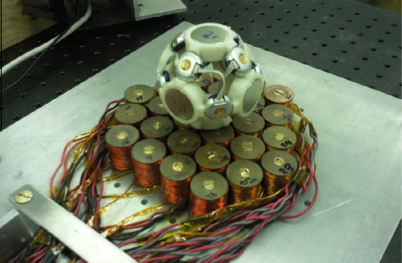
\includegraphics[width=0.45\textwidth]{Moving_Magnet_1}}
\hspace{2mm}
\subfloat[سیم‌پیچ‌های سه فاز
\cite{RN24}]
{ \label{fig:Moving_Magnet_2}
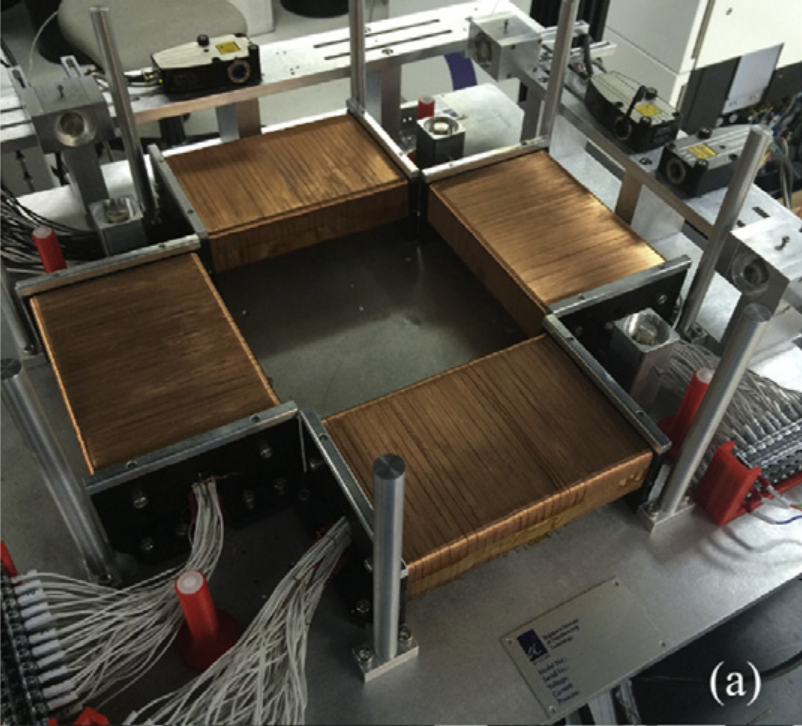
\includegraphics[width=0.45\textwidth]{Moving_Magnet_2}}
\\ % Newline to wrap the figures to the next row
\subfloat[ساختار دوگانه سیم‌پیچ‌ها
\cite{RN32}]
{ \label{fig:Moving_Magnet_3}
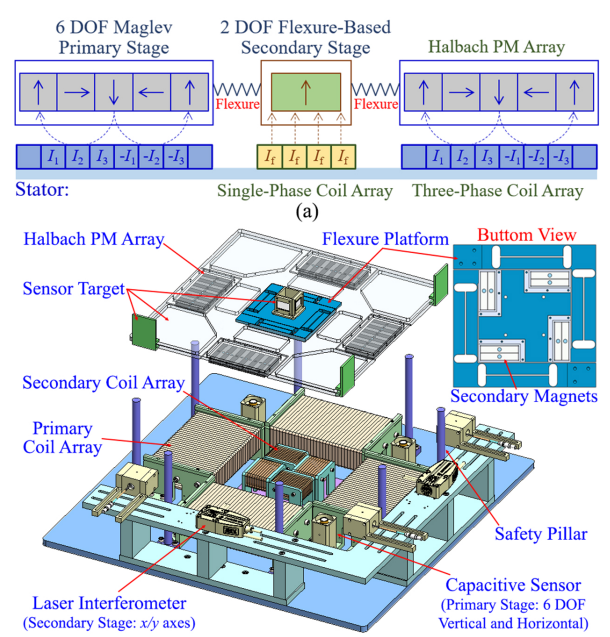
\includegraphics[width=0.45\textwidth]{Moving_Magnet_3}}
\hspace{2mm}
\subfloat[ساختار ماژولار سیم‌پیچ‌ها
\cite{RN10}]
{ \label{fig:Moving_Magnet_4}
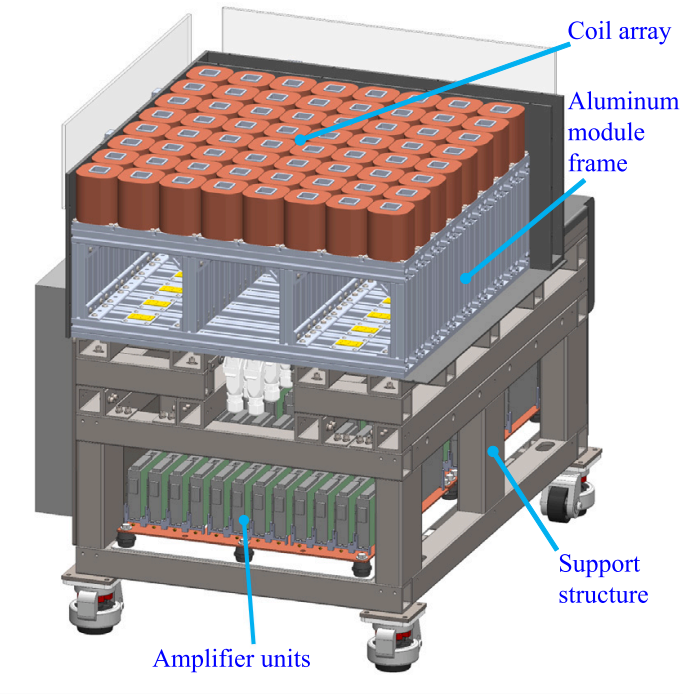
\includegraphics[width=0.45\textwidth]{Moving_Magnet_4}}
\label{fig:Moveing_Magnet} %% label for entire figure
\caption{ساختارهای آهنرباهای متحرک و سیم‌پیچ‌های ثابت}
\end{figure}








\section{ساختار آهنرباهای دائمی}

همان‌طور که در بخش قبل اشاره شد، میدان مغناطیسی کنترل‌شده توسط آهنرباهای الکتریکی ایجاد می‌شود و بر اثر تعامل این میدان متغیر با میدان ثابت آهنرباهای دائمی، نیرویی بر بخش متحرک دستگاه وارد می‌شود که حرکت آن را در راستاهای مختلف ممکن می‌سازد. بنابراین، طراحی بهینه آهنرباهای دائمی، به‌ویژه برای تولید میدان مغناطیسی قوی‌تر با کمترین وزن، در بهبود کارایی دستگاه نقش کلیدی دارد. در این بخش، طراحی‌های مختلف آهنرباهای دائمی که در پژوهش‌های پیشین ارائه شده‌اند، با تمرکز بر بهینه‌سازی این ویژگی‌ها بررسی می‌شوند.
\subsection{استفاده از آهنرباهای دیسکی}

استفاده از آهنرباهای دیسکی رویکردی ساده و مؤثر برای ایجاد میدان مغناطیسی دائمی محسوب می‌شود. با انتخاب موادی با خاصیت مغناطیسی بالا، مانند آهنرباهای نئودیمیومی، می‌توان به شدت میدان مغناطیسی مطلوب دست یافت. به عنوان نمونه، در پژوهش 
\cite{RN7}
 از دو آهنربای دیسکی جهت تأمین میدان مغناطیسی ثابت استفاده شده است. همچنین در پژوهش 
\cite{RN39}
 با به‌کارگیری ۶ آهنربای دیسکی، امکان چرخش آزادانه حول سه محور فراهم شده است.(شکل
\ref{fig:Disk_Magnet_1})
 در پژوهش 
\cite{RN8}
 نیز از ترکیب‌های متفاوتی از آهنرباهای دیسکی برای بخش متحرک دستگاه استفاده شده است، که این ترکیب‌ها شامل تغییر اندازه‌ی یک آهنربا و استفاده از سه آهنربای دیسکی است. سیستم شناوری مغناطیسی با پنج درجه آزادی که تنها از یک آهنربای دیسکی تشکیل شده است، در پژوهش 
\cite{RN62}
 به عنوان نمونه‌ای موفق از این رویکرد معرفی شده است. این طراحی، با وجود سادگی معماری، توانسته نتایج رضایت‌بخشی را از نظر عملکرد ارائه دهد و نشان می‌دهد که استفاده از آهنربای دیسکی، علاوه بر سادگی، می‌تواند در کاربردهای مختلف به‌ویژه در سیستم‌های با نیاز به دقت بالا و چند درجه آزادی، کارآمد باشد. شکل((
\ref{fig:Disk_Magnet_2})


\begin{figure}[ht]
\centering 
\subfloat[دو آهنربای دیسکی
\cite{RN7}]
{ \label{fig:Disk_Magnet_1}
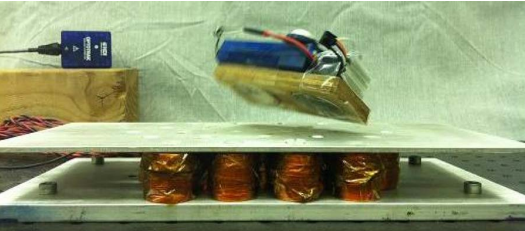
\includegraphics[width=0.5\textwidth]{Disk_Magnet_1}}
%\hspace{2mm}
\subfloat[یک آهنربای دیسکی
\cite{RN62}]
{ \label{fig:Disk_Magnet_2}
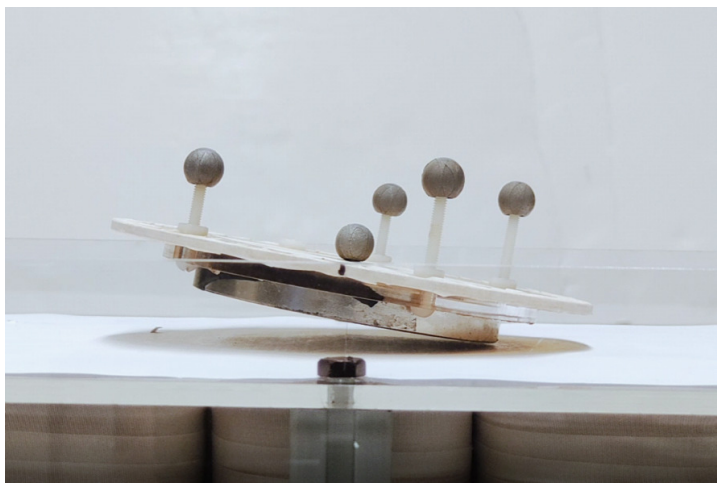
\includegraphics[width=0.5\textwidth]{Disk_Magnet_2}}%
\caption{استفاده از آهنربای دیسکی در طراحی متحرک}
\label{fig:Disk_Magnet} %% label for entire figure
\end{figure}



\subsection{آرایه‌ی هالباخ یک بعدی}

آرایه‌ی هالباخ
\LTRfootnote{Halbach Array}
 به‌عنوان چینشی از آهنرباهای دائمی تعریف می‌شود که در آن جهت مغناطیس‌شوندگی هر آهنربا با آهنربای مجاور خود ۹۰ درجه تفاوت دارد. این آرایه به‌طور خاص قادر است میدان مغناطیسی در یک سوی آرایه را خنثی کرده و در سوی دیگر میدان را به میزان تقریبی 1.4 برابر افزایش دهد.
مزیت این ساختار در طراحی سیستم‌های MLPM، توانایی آن در تولید شدت میدان مغناطیسی بیشتر است. به‌همین‌دلیل، این چینش در بسیاری از پژوهش‌ها مورد استفاده قرار گرفته است.
با این حال، استفاده از تنها یک آرایه‌ی یک‌بعدی هالباخ به‌تنهایی نمی‌تواند نیرویی در دو راستای افقی ایجاد کند. لذا معمولاً از تعداد بیشتری از این آرایه‌ها در ساختار متحرک استفاده می‌شود. به‌عنوان مثال، در پژوهش‌های 
\cite{RN24,RN27}
 از چهار آرایه‌ی هالباخ یک‌بعدی در بخش متحرک استفاده شده است که هر یک از این آرایه‌ها قادر به ایجاد نیرویی در یکی از راستاهای افقی و عمودی هستند.
در پژوهش 
\cite{RN39}
، مشابه آنچه که در بخش استاتور پیاده‌سازی شده بود، از ساختار دوگانه‌ای در بخش متحرک بهره‌برداری شده است، به‌گونه‌ای که دو مجموعه چهارگانه از آرایه‌های هالباخ در معماری این بخش به‌کار رفته‌اند.

\begin{figure}[ht]
\centering 
\subfloat[آرایه‌ی هالباخ
\cite{RN16}]
{ \label{fig:halbach1D}
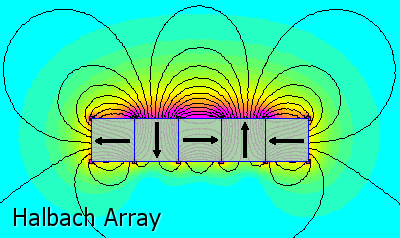
\includegraphics[width=0.5\textwidth]{halbach1D}}
%\hspace{2mm}
\subfloat[4 آرایه‌ی یک بعدی هالباخ
\cite{RN39}]
{ \label{fig:4_halbach1D_array}
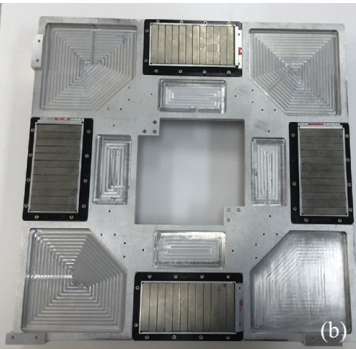
\includegraphics[width=0.5\textwidth]{4_halbach1D_array}}%
\caption{آرایه هالباخ یک‌بعدی}
\label{fig:halbach1D} %% label for entire figure
\end{figure}

\subsection{آرایه هالباخ دوبعدی}

برای رفع محدودیت‌های آرایه‌ی هالباخ یک‌بعدی که تنها در یک راستا نیرو ایجاد می‌کند، ساختار جدیدی از آرایه‌ی دوبعدی ارائه شده است. این آرایه قادر است میدان مغناطیسی را در یک طرف صفحه حذف و در طرف دیگر تقویت کند. با این ویژگی، استفاده از چندین آرایه برای تأمین میدان مغناطیسی ثابت ضروری نخواهد بود. طراحی آرایه‌ی دوبعدی در بسیاری از پژوهش‌ها برای بخش‌های متحرک یا استاتور سیستم‌های MLPM به کار گرفته شده است.

استفاده از آرایه‌ی هالباخ در پژوهش‌های مختلفی از جمله
\cite{RN10, RN30} 
و
\cite{RN55, RN26} 
نشان‌دهنده‌ی عملکرد بهینه‌ی این معماری در بخش متحرک سیستم‌های MLPM است.(شکل
\ref{fig:halbach2D_2})
 همچنین در پژوهش
\cite{RN14}
 از این آرایه به عنوان بخشی از استاتور دستگاه بهره‌گیری شده است. در 
\cite{RN61}
 ماژول‌هایی برای ساخت این آرایه استفاده شده (شکل
\ref{fig:halbach2D_4})
 و در
\cite{RN49}
 برای تشکیل آرایه از قطعات آهنی در فضای خالی میان آن استفاده شده است؛ اما این رویکرد باعث ایجاد خطا در دقت میدان مغناطیسی شده است. (شکل
\ref{fig:halbach2D_3})
علاوه بر این، در پژوهش
\cite{RN28}
، طراحی جدیدی با آهنرباهایی با میزان مغناطیس‌شوندگی و ارتفاع متفاوت پیشنهاد شده است.
\begin{figure}[ht]
\centering 
\subfloat[آرایه هالباخ دو بعدی و میدان مغناطیسی آن
\cite{RN10}]
{ \label{fig:halbach2D_2}
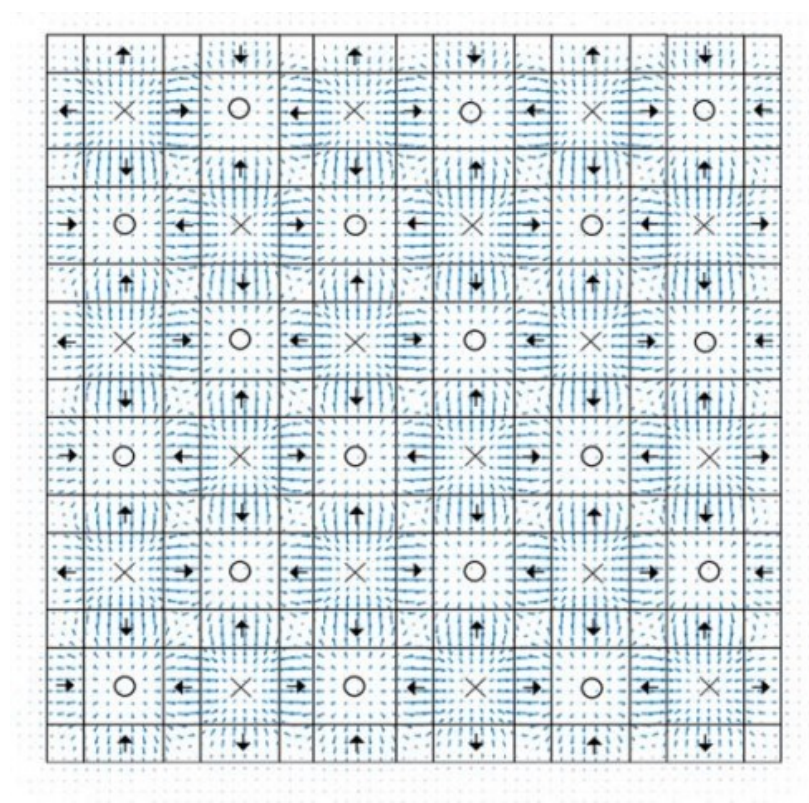
\includegraphics[width=0.45\textwidth]{halbach2D_2}}
\hspace{2mm}
\subfloat[آرایه هالباخ دوبعدی با قطعات آهنی در فضاهای خالی
\cite{RN49}]
{ \label{fig:halbach2D_3}
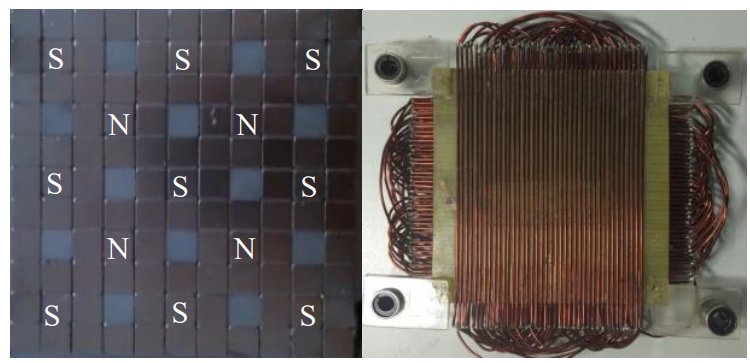
\includegraphics[width=0.45\textwidth]{halbach2D_3}}
\\ % Newline to wrap the figures to the next row
\subfloat[آرایه هالباخ دوبعدی ماژولار
\cite{RN61}]
{ \label{fig:halbach2D_4}
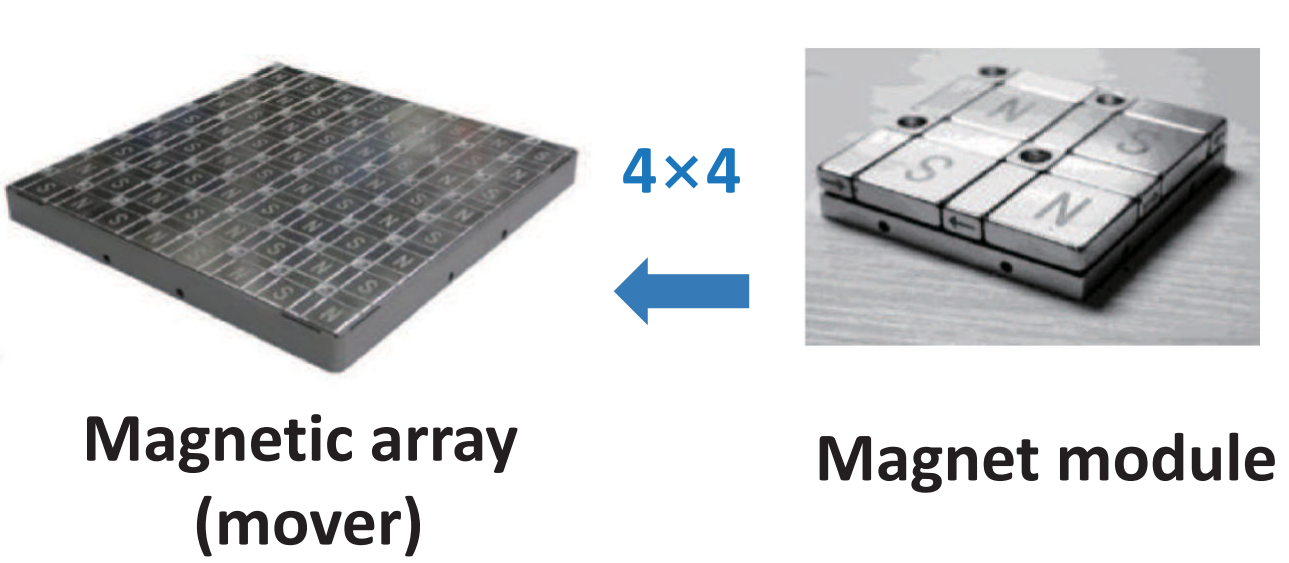
\includegraphics[width=0.45\textwidth]{halbach2D_4}}
\caption{آرایه هالباخ دو‌بعدی}
\label{fig:halbach2D} %% label for entire figure

\end{figure}
\section{طراحی کنترلر}
همان‌طور که پیش‌تر اشاره شد، سیستم‌های شناوری مغناطیسی ذاتاً ناپایدار هستند و برای دستیابی به پایداری، به کنترلری با عملکرد دقیق و خطای کم نیاز است. در پژوهش‌های مختلف، از کنترلرهای گوناگونی برای این سیستم‌ها بهره گرفته شده است؛ از جمله کنترلرهای کلاسیک نظیر PID، کنترلرهای مدرن مانند کنترل مبتنی بر پیش‌بینی مدل (MPC) و همچنین مدل‌های مبتنی بر هوش مصنوعی نظیر شبکه‌های بازگشتی GRU. در این بخش، به بررسی این کنترلرها و مقایسه‌ عملکرد آنها خواهیم پرداخت.
\subsection{کنترلر PID}

کنترل تناسبی-انتگرالی-مشتقی (PID) به عنوان یکی از پرکاربردترین و موثرترین کنترلرهای کلاسیک در سیستم‌های دینامیکی، گزینه‌ای مناسب برای کنترل سیستم‌های MLPM محسوب می‌شود. این کنترلر به دلیل سادگی در پیاده‌سازی، تنظیم دقیق و توانایی تنظیم خروجی سیستم بر اساس خطاهای ورودی، به‌طور گسترده در سیستم‌های مختلف استفاده شده است. برای کنترل سیستم‌های MLPM، به ازای هر درجه آزادی یک کنترلر PID طراحی و پیاده‌سازی می‌شود تا بتواند جریان الکتریکی سیم‌پیچ‌ها را تنظیم کرده و میدان مغناطیسی لازم برای ایجاد و حفظ موقعیت متحرک را تأمین کند.

در پژوهش‌های متعددی از کنترلر PID برای سیستم‌های MLPM بهره گرفته شده است. به عنوان مثال، در 
\cite{RN39,RN24}
از کنترلرهای PID ساده برای کنترل جریان سیم‌پیچ‌ها استفاده شده که وظیفه تنظیم میدان مغناطیسی و در نتیجه، کنترل موقعیت جسم متحرک را بر عهده دارند. علاوه بر این، در پژوهش
\cite{RN32}
، از دو کنترلر PID در یک ساختار دوگانه استفاده شده است. کنترلر اول برای جابه‌جایی‌های بلند و در مسافت‌های طولانی به کار رفته و جریان سیم‌پیچ‌های اصلی را تنظیم می‌کند، در حالی که کنترلر دوم برای حرکات دقیق کوتاه‌برد طراحی شده و کنترل جریان سیم‌پیچ‌های ثانویه را بر عهده دارد. این روش باعث بهینه‌سازی کنترل دقیق و بهبود دقت در حرکات کوتاه‌برد و جابه‌جایی‌های سریع می‌شود.
همچنین در سیستم MagTable، برای کنترل دقیق موقعیت آهنرباهای دائمی، از شش کنترلر PID به‌صورت همزمان استفاده شده است تا نیروی متوازن برای پایدارسازی موقعیت متحرک در چندین جهت فراهم شود 
\cite{RN8}
. این نوع طراحی و استفاده از کنترلرهای PID نشان می‌دهد که علی‌رغم محدودیت‌های موجود در کنترلرهای کلاسیک، این روش همچنان در بسیاری از سیستم‌های مغناطیسی پیچیده مانند MLPM کارایی بالایی دارد.

\begin{figure}[ht]
\centering{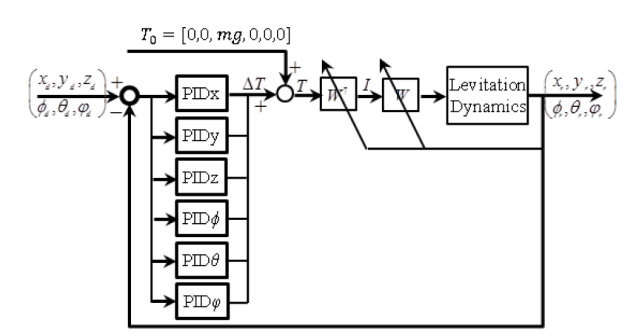
\includegraphics[width=0.5\textwidth]{PID_1}}
\caption{کنترلر PID با 6 درجه آزادی
\cite{RN8}}
\label{fig:PID}
\end{figure}


\subsection{کنترلر مبتنی بر پیش‌بینی مدل MPC}
برای کنترل سیستم‌های MLPM اگر مدل سیستم به روش‌های تحلیلی و یا عددی به دست آمده و تخمین زده شده باشد، می‌توان از این مدل‌ها برای طراحی کنترلرهای پیشرفته‌تر با هدف پیش‌بینی رفتار سیستم و استفاده از آن به صورت پیش‌خور در حلقه‌ی کنترلی استفاده کرد. روش‌های تخمین مدل این سیستم‌ها در بخش‌های بعد مورد بررسی قرار می‌گیرد. در این بخش، کنترلرهای ارائه شده در پژوهش‌های دیگر ارائه می‌شود.
به دست آوردن معادلات دینامیکی سیستم و استفاده از آنها در پیش‌بینی روشی تحلیلی است که در 
\cite{RN55}
 استفاده شده است و مدل کنترلی متشکل از بلوک‌های پس‌خور و پیش‌خور برای کنترل موقعیت آهنربا طراحی شده است. همچنین در 
\cite{RN62}
 از یک جدول جستجو برای تعیین رفتار سیستم در نقاط مختلف فضا استفاده شده است که این جدول به عنوان پیش‌خور به مدل کنترلی داده می‌شود. در ادامه‌ی این پژوهش، با استفاده از روش‌های شناسایی سیستم، مدلی تقریبی برای رفتار سیستم در نظر گرفته شده است و با استفاده از این مدل برای پیش‌بینی رفتار سیستم‌ مدل MPC پیاده‌سازی شده است. پژوهش 
\cite{RN30}
 با تمرکز بر ارائه‌ی یک مدل پیش‌بین، با استفاده از معادلات دینامیکی سیستم و همچنین روش‌پیش‌بینی حالت بی‌تاخیر، رفتار آینده‌ی سیستم را محاسبه می‌کند.
\begin{figure}[ht]
\centering 
\subfloat[\cite{RN55}]{
    \label{fig:MPC_1}
    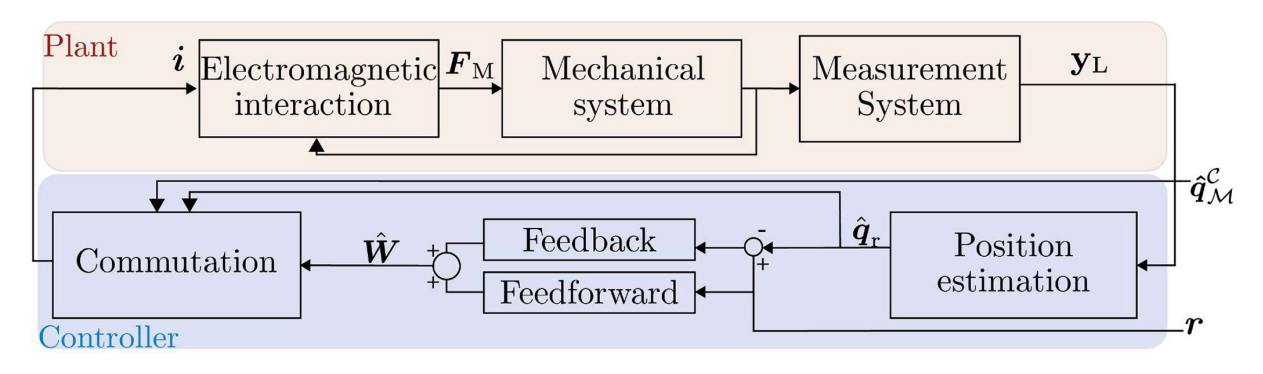
\includegraphics[width=0.45\textwidth]{MPC_1}}
%\hspace{2mm}
\subfloat[\cite{RN62}]{
    \label{fig:MPC_2}
    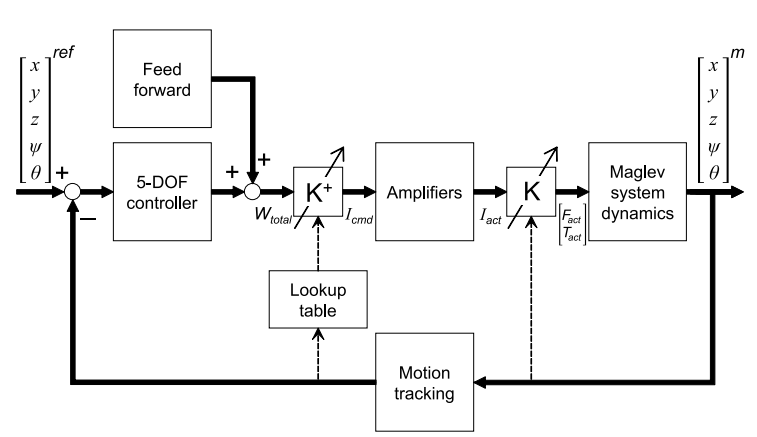
\includegraphics[width=0.45\textwidth]{MPC_2}}
\\ % Newline to wrap the figures to the next row
\subfloat[\cite{RN61}]{
    \label{fig:MPC_3}
    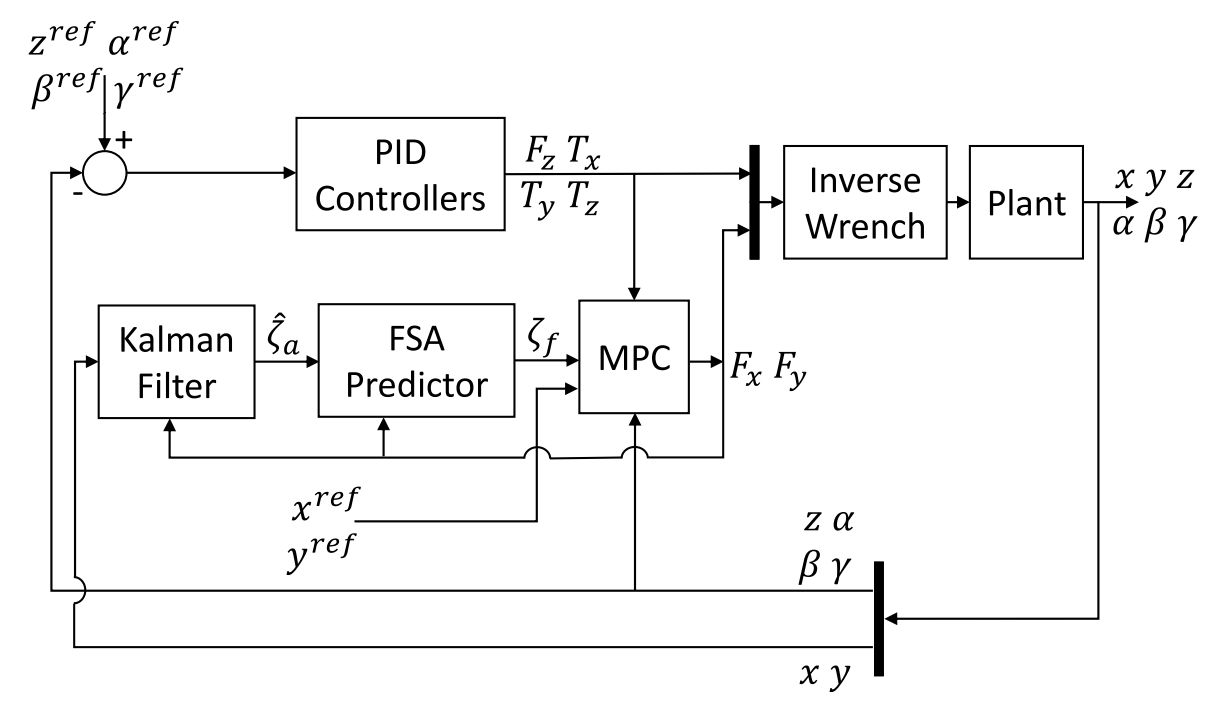
\includegraphics[width=0.45\textwidth]{MPC_3}}
\subfloat[\cite{RN61}]{
    \label{fig:MPC_4}
    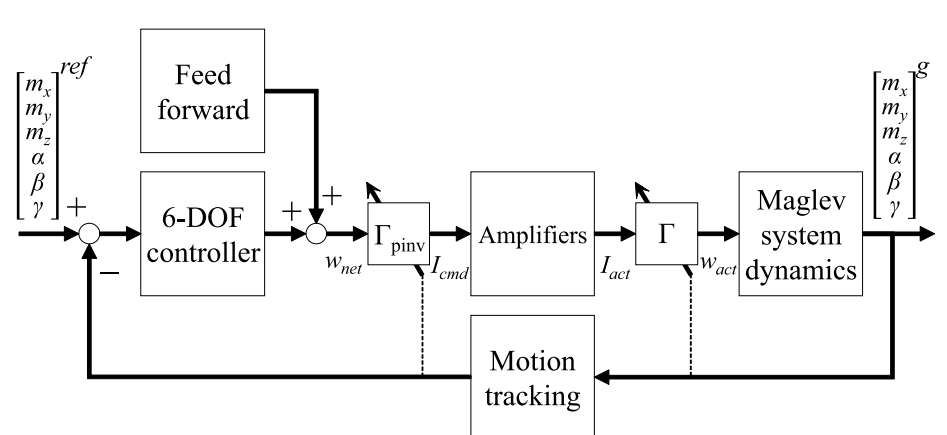
\includegraphics[width=0.45\textwidth]{MPC_4}}
\caption{کنترلر MPC}
\label{fig:MPC} %% label for entire figure
\end{figure}

\FloatBarrier

\subsection{کنترلر مبتنی بر هوش مصنوعی}

یکی از روش‌های نوین برای پیش‌بینی رفتار سیستم‌های پیچیده مانند MLPM، استفاده از مدل‌های هوش مصنوعی به‌ویژه شبکه‌های عصبی بازگشتی (RNN) است. این مدل‌ها با یادگیری دینامیک سیستم و ارتباط بین ورودی‌ها و خروجی‌ها، می‌توانند به‌طور مؤثری رفتار سیستم را در شرایط مختلف پیش‌بینی کنند. در این راستا، پژوهش
\cite{RN61}
از یک مدل بازگشتی GRU 
\LTRfootnote{Gated Recurrent Unit}
 استفاده کرده است. این مدل بر اساس داده‌های جمع‌آوری‌شده از عملکرد دستگاه MLPM آموزش دیده و توانسته است با دقت بالا تغییرات دینامیکی سیستم و پاسخ آن به ورودی‌های گوناگون را پیش‌بینی کند. استفاده از GRU به دلیل توانایی آن در مدل‌سازی وابستگی‌های زمانی و در نظر گرفتن اطلاعات قبلی برای پیش‌بینی‌های دقیق‌تر، رویکردی مناسب در این پژوهش بوده است.(شکل 
\ref{fig:GRU}

\begin{figure}[ht]
\centering
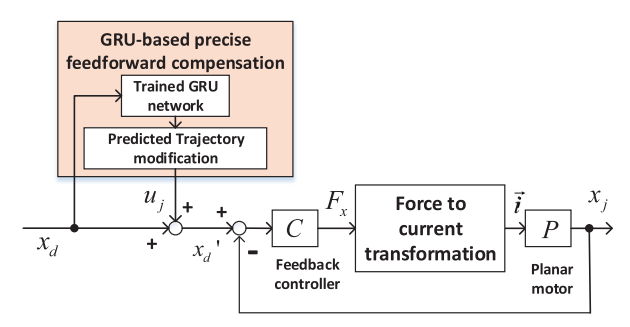
\includegraphics[width=0.5\textwidth]{GRU_1}
\caption{کنترلر پیش‌خور GRU \cite{RN61}}
\label{fig:GRU}
\end{figure}

\section{مدل‌سازی و تخمین سیستم}
در روش بار نقطه‌ای برای تحلیل میدان مغناطیسی، فرض می‌شود که توزیع بار مغناطیسی در یک حجم به‌صورت متمرکز در هشت نقطه در گوشه‌های آن حجم قرار گرفته است. با این فرض، اثر مغناطیسی این جسم می‌تواند به‌صورت مجموع آثار هر یک از بارهای نقطه‌ای محاسبه شود. این رویکرد امکان محاسبه‌ی دقیق شدت میدان مغناطیسی و نیروی وارد بر یک جسم خارجی را فراهم می‌آورد. از طریق محاسبه‌ی میدان‌های ناشی از هر بار نقطه‌ای و جمع آنها، میدان مغناطیسی کل حاصل می‌شود و به این ترتیب، شدت میدان مغناطیسی ناشی از آهنربای دائمی به کمک این روش به‌طور دقیق محاسبه می‌گردد. در ادامه، معادلات مربوط به محاسبه‌ی شدت میدان مغناطیسی ارائه شده‌اند.
\subsection{مدل بار مغناطیسی سطحی}
در این مدل، فرض بر این است که بار مغناطیسی در یک المان حجم سه‌بعدی به‌صورت توزیعی از بارهای مغناطیسی با چگالی بار J بر روی دو صفحه‌ی موازی قرار گرفته است. با استفاده از این فرض، میدان مغناطیسی ایجادشده توسط این حجم به‌صورت میدان حاصل از توزیع بارهای مغناطیسی محاسبه می‌شود. این مدل امکان تحلیل دقیق‌تر رفتار میدان مغناطیسی را فراهم می‌کند. مقایسه نتایج حاصل از این مدل با شبیه‌سازی المان محدود
\LTRfootnote{Finite Element Method (FEM)}
 در پژوهش
\cite{RN44}
نشان داده است که این روش مدل‌سازی برای سیستم‌های MLPM دقت و کارایی بالایی دارد.

\begin{figure}[ht]
\centering
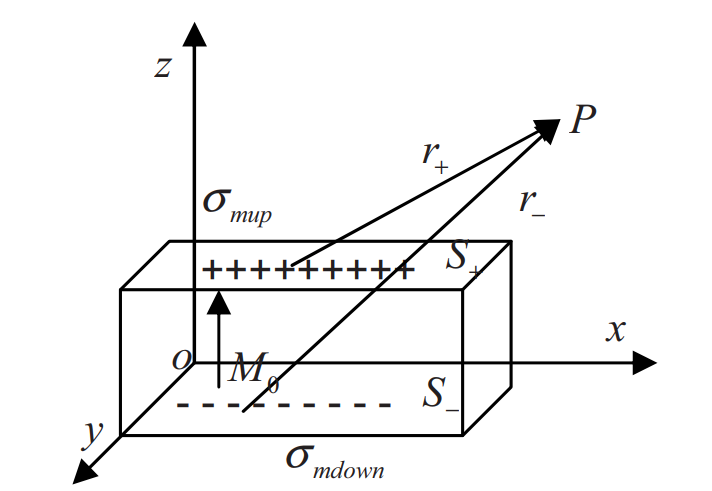
\includegraphics[width=0.5\textwidth]{Magnetic surface charge_2}
\caption{مدل بار مغناطیسی سطحی \cite{RN44}}
\label{fig:Magnetic surface charge}
\end{figure}

\subsection{مدل بار مغناطیسی نقطه‌ای}
در روش بار نقطه‌ای برای تحلیل میدان مغناطیسی، فرض می‌شود که توزیع بار مغناطیسی در یک حجم به‌صورت متمرکز در هشت نقطه در گوشه‌های آن حجم قرار گرفته است. با این فرض، اثر مغناطیسی این جسم می‌تواند به‌صورت مجموع آثار هر یک از بارهای نقطه‌ای محاسبه شود. این رویکرد امکان محاسبه‌ی دقیق شدت میدان مغناطیسی و نیروی وارد بر یک جسم خارجی را فراهم می‌آورد. از طریق محاسبه‌ی میدان‌های ناشی از هر بار نقطه‌ای و جمع آنها، میدان مغناطیسی کل حاصل می‌شود و به این ترتیب، شدت میدان مغناطیسی ناشی از آهنربای دائمی به کمک این روش به‌طور دقیق محاسبه می‌گردد. در ادامه، معادلات مربوط به محاسبه‌ی شدت میدان مغناطیسی ناشی از هر بار نقطه‌ای ارائه شده‌است.
\begin{align}
B_{xk} &= \frac{\epsilon_k}{4\pi} \ln\left(-y_r + \sqrt{x_r^2 + y_r^2 + z_r^2}\right), \\
B_{yk} &= \frac{\epsilon_k}{4\pi} \ln\left(-x_r + \sqrt{x_r^2 + y_r^2 + z_r^2}\right), \\
B_{zk} &= \frac{\epsilon_k}{4\pi} \arctan\left( \frac{x_r y_r}{\sqrt{x_r^2 + y_r^2 + z_r^2}} \right),
\end{align}

\begin{figure}[ht]
\centering
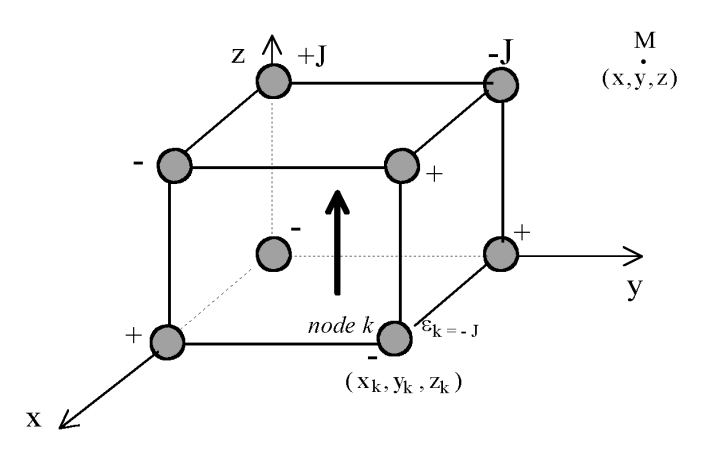
\includegraphics[width=0.5\textwidth]{Magnetic_Node}
\caption{مدل بار مغناطیسی نقطه‌ای \cite{RN44}}
\label{figMagnetic_Node}
\end{figure}

\subsection{مدل های مبتنی بر داده}

در این روش‌ها، به‌جای مدل‌سازی دقیق ساختار فیزیکی دستگاه و استخراج معادلات دینامیکی آن، پارامترهای مورد نیاز مانند شدت میدان مغناطیسی از طریق داده‌های تجربی یا شبیه‌سازی المان محدود (FEM) تخمین زده می‌شوند. این رویکرد مبتنی بر داده نیازمند دسترسی به اطلاعات دقیق از سیستم واقعی یا شبیه‌سازی کامل آن است تا بتوان دقت و اعتبار تخمین‌ها را ارزیابی کرد. در پژوهش 
\cite{RN10}
، برای تخمین شدت میدان مغناطیسی آرایه هالباخ دوبعدی از معادلات هارمونیک و سری فوریه استفاده شده است. تغییرات میدان مغناطیسی تولیدشده توسط این آرایه به‌صورت موجی سینوسی مدل‌سازی شده است، اما این روش تنها زمانی دقیق است که فرض شود سطح آرایه به‌صورت نامحدود ادامه دارد. برای حل این مشکل، آرایه به سه ناحیه مرکزی، کناری و گوشه‌ای تقسیم‌بندی شده و برای هر ناحیه هارمونیک‌های مجزا در نظر گرفته شده است. نتایج این پژوهش نشان می‌دهند که با استفاده از سه هارمونیک اول، می‌توان میدان مغناطیسی را در نواحی کناری و گوشه‌ای با دقت مناسبی تخمین زد.

\begin{figure}[ht]
\centering 
\subfloat[\cite{RN10}]{
\label{fig:harmonic_1}
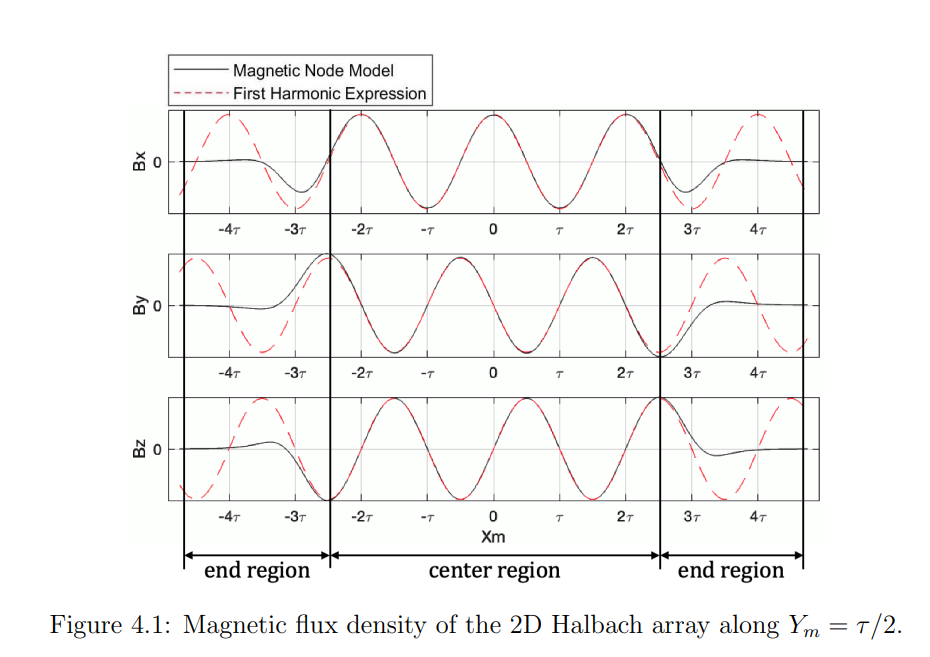
\includegraphics[width=0.45\textwidth]{harmonic_1}}
\hspace{2mm}
\subfloat[\cite{RN10}]{
\label{fig:harmonic_2}
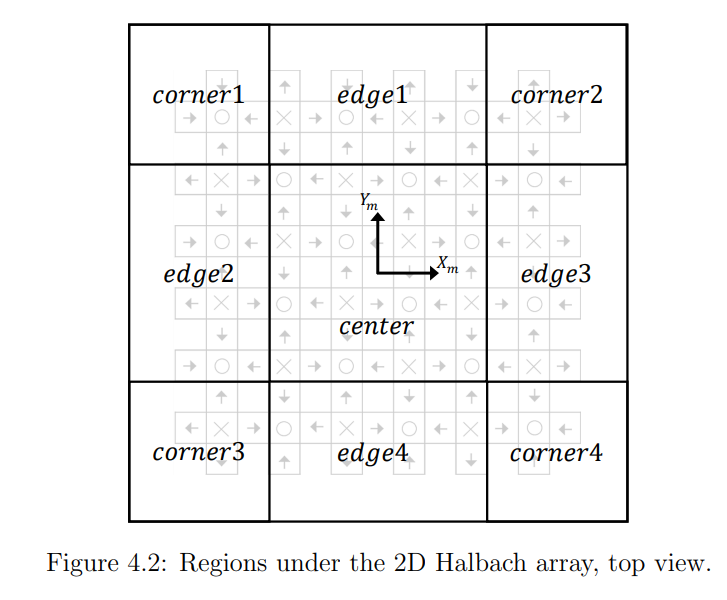
\includegraphics[width=0.45\textwidth]{harmonic_2}}
\caption{مدل هارمونیک}
\label{fig:harmonic}
\end{figure}



!
را در فایل 
\lr{main.tex}،
غیرفعال%
\footnote{
برای غیرفعال کردن یک دستور، کافی است در ابتدای آن، علامت درصد انگلیسی (\%) بگذارید.
}
 کنید. در غیر این صورت، ابتدا مطالب دو فصل اول پردازش شده و سپس مطالب فصل ۳ پردازش می‌شود که این کار باعث طولانی شدن زمان پردازش می‌گردد. هر زمان که خروجی کل \پ را خواستید، تمام فصل‌ها را دوباره در
\lr{main.tex}
فعال نمائید.
بدیهتاً لازم نیست فصل‌های \پ را به ترتیب تایپ کنید. مثلاً می‌توانید ابتدا مطالب فصل ۳ را تایپ نموده و سپس مطالب فصل ۱ را تایپ کنید. 
\subsubsection{مراجع}
برای وارد کردن مراجع \پ کافی است فایل 
\lr{MyReferences.bib}
را باز کرده و مراجع خود را به شکل اقلام نمونهٔ داخل آن، وارد کنید.  سپس از \lr{bibtex} برای تولید مراجع با قالب مناسب استفاده نمائید. برای توضیحات بیشتر بخش \ref{Sec:Ref} از پیوست \ref{app:latexIntro} و نیز پیوست \ref{app:refMan} را ببینید.

\subsubsection{واژه‌نامه فارسی به انگلیسی و برعکس}
برای وارد کردن معادل فارسی اصطلاحات لاتین در متن و تهیه فهرست واژه‌نامه از آنها، از بستهٔ
\lr{glossaries}
و نرم‌افزار
\lr{xindy}
استفاده می‌شود. بدین منظور کافی است اصطلاحات لاتین و ترجمهٔ آنها را در فایل
\lr{words.tex}
وارد کرده و هر جای متن که خواستید با دستورات
\verb|gls{label}|
یا \verb|glspl{label}|
معادل فارسی مفرد یا جمع یک اصطلاح را بیاورید.

مثلا در اینجا، واژهٔ
«\gls{Action}»
برای بار اول و دوباره
«\gls{Action}»
برای بار دوم در متن ظاهر شده است.
جهت توضیحات بیشتر به پیوست
\ref{app:refMan}
مراجعه کنید.
\subsubsection{نمایه}
برای وارد کردن نمایه، باید از 
\lr{xindy}
استفاده کنید. 
%زیرا 
%\lr{MakeIndex}
%با حروف «گ»، «چ»، «پ»، «ژ» و «ک» مشکل دارد و ترتیب الفبایی این حروف را رعایت نمی‌کند. همچنین، فاصله بین هر گروه از کلمات در 
%\lr{MakeIndex}،
%به درستی رعایت نمی‌شود که باعث زشت شدن حروف‌چینی این قسمت می‌شود. 
راهنمای چگونگی کار با 
\lr{xindy} 
را می‌توانید در ویکی پارسی‌لاتک و یا مثالهای موجود در دی‌وی‌دی «مجموعه پارسی‌لاتک»، پیدا کنید.

\subsection{اگر سوالی داشتم، از کی بپرسم؟}
برای پرسیدن سوال‌های خود موقع حروف‌چینی با زی‌پرشین، می‌توانید به
\href{http://qa.parsilatex.com}{سایت پرسش و پاسخ پارسی‌لاتک}%
\LTRfootnote{http://qa.parsilatex.com}
یا
\href{http://forum.parsilatex.com}{بایگانی تالارگفتگوی قدیمی پارسی‌لاتک}%
\LTRfootnote{http://forum.parsilatex.com}
مراجعه کنید. شما هم می‌توانید روزی به سوال‌های دیگران در اینترنت جواب دهید.
بستهٔ زی‌پرشین و بسیاری از بسته‌های مرتبط با آن مانند
\lr{bidi} و
\lr{Persian-bib}،
مجموعه پارسی‌لاتک، مثالهای مختلف موجود در آن، قالب پایان‌نامه دانشگاههای مختلف و سایت پارسی‌لاتک همه به صورت داوطلبانه توسط افراد گروه پارسی‌لاتک و گروه
\lr{Persian TeX}
و بدون هیچ کمک مالی انجام شده‌اند. کار اصلی نوشتن و توسعه زی‌پرشین توسط آقای وفا خلیقی انجام شده است که این کار بزرگ را به انجام رساندند.
اگر مایل به کمک به گروه پارسی‌لاتک هستید به سایت این گروه مراجعه فرمایید:
\begin{center}
	\url{http://www.parsilatex.com}
\end{center}

\section{محتویات فصل اول یک پایان‌نامه}
فصل اول یک پایان‌نامه باید به مقدمه یا کلیات تحقیق بپردازد.
هدف از فصل مقدمه%
\LTRfootnote{Introduction}،
شرح مختصر مسأله تحقیق، اهمیت و انگیزه محقق از پرداختن به آن موضوع، بهمراه اشاره‌ای کوتاه به روش و مراحل تحقیق است. مقدمه، اولین فصل از ساختار اصلی \پ بوده و زمینه اطلاعاتی لازم را برای خواننده فراهم می‌آورد. در طول مقدمه باید سعی شود موضوع تحقیق با زبانی روشن، ساده و بطور عمیق و هدفمند به خواننده معرفی شود. این فصل باید خواننده را مجذوب و اهمیت موضوع تحقیق را آشکار سازد. در مقدمه باید با ارائهٔ سوابق، شواهد تحقیقی و اطلاعات موجود (با ذکر منبع) با روشی منظم، منطقی و هدف‌دار، خواننده را جهت داد و به سوی راه حل مورد نظر هدایت کرد. مقدمه مناسب‌ترین جا برای ارائهٔ اختصارات و بعضی توضیحات کلی است، توضیحاتی که شاید نتوان در مباحث دیگر آنها را شرح داد.

مقدمه، یکی از ارکان اساسی و اصلی پایان نامه است که مهمترین قسمت‌های آن عبارتند از: 

\subsection{عنوان تحقیق} 
باید شناختی دقیق و روشن از حوزهٔ موضوع تحقیق را عرضه دارد و خالی از هرگونه ابهام و پیچیدگی باشد.

\subsection{مسأله تحقیق}
وظیفه اصلی مقدمه بیان این مطلب به خواننده است که چرا انجام تحقیق را به عهده گرفته‌اید. اگر دلیل شما برای انجام این کار پاسخگویی به سؤال مورد علاقه‌تان است، با مشکل زیادی روبه‌رو نخواهید بود. یکی از بهترین روش‌ها برای نوشتن مقدمهٔ یک پایان‌نامه، طرح پرسش یا پرسش‌هایی مهم و اساسی است که کار تحقیقاتی شما از آغاز تا پایان قصد پاسخ دادن به آن را دارد. گاهی می‌توانید ابتدا اهمیت موضوع را بیان و سپس پرسش خود را در آن موضوع مطرح کنید.

\subsection{تاریخچه‌ای از موضوع تحقیق}
به طور کلی تشریح روندهای تحقیقاتی در محدودهٔ مورد مطالعه، مستلزم ارجاع به کارهای دیگران است. بعضی از نویسندگان برای کارهای دیگران هیچ اعتباری قائل نمی‌شوند و در مقابل، بعضی دیگر از نویسندگان در توصیف کارهای دیگران، بسیار زیاده‌روی می‌کنند. اکثر مواقع، ارجاع به مقالات دو سال قبل از کارتان، بهتر از نوشتن سطرهای مرجع است. در این قسمت باید به طور مختصر به نظرات و تحقیقات مربوط به موضوع و یا مسائل و مشکلات حل نشده در این حوزه و همچنین توجه و علاقه جامعه به این موضوع، اشاره شود.

\subsection{تعریف موضوع تحقیق}
در این قسمت محقق، موضوع مورد علاقه و یا نیاز احساس شدهٔ خود را در حوزه تحقیق بیان می‌دارد و عوامل موجود در موقعیت را تعریف و تعیین می‌کند.

\subsection{هدف یا هدف‌های کلی و آرمانی تحقیق}
این قسمت باید با جملات مثبت و کلی طرح شود و از طولانی شدن مطالب پرهیز شود.

\subsection{روش انجام تحقیق}
در این قسمت، پژوهشگر روش کاری خود را بیان می‌دارد و شیوه‌های گوناگونی را که در گردآوری مطالب خود بکار برده، ذکر می‌کند. همچنین اگر روش آماری خاصی را در تهیه و تدوین اطلاعات به کار برده است، آن شیوه را نیز اینجا بیان می‌کند.

\subsection{نوآوری، اهمیت و ارزش تحقیق}
در این قسمت، در مورد نوآوری علمی و عملی تحقیق که محقق به آن دست خواهد یافت، بحث می‌شود. ممکن است لازم باشد تا برخی نمودارهای خلاصه در این بخش استفاده شوند. به عنوان مثال، نموداری از مقاله
\cite{kim2016integrated}
در شکل
\ref{fig:sampleDiagram}
آمده است.
\begin{figure}[ht]
	\centerline{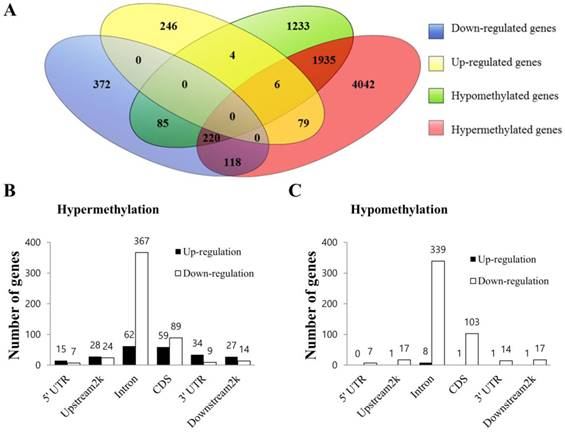
\includegraphics[width=0.8\textwidth]{journal-of-cancer_sample-result}}
	\caption{یک نمونه نمودار خلاصه برای نمایش نوآوری در نتایج
		%\cite{kim2016integrated}
	}
	\label{fig:sampleDiagram}
\end{figure}\\
طبیعتاً به صلاحدید نگارنده، شکل‌ها و نمودار‌ها می توانند در بخش های مختلف، خصوصا فصل
\ref{chap:results}
مورد استفاده قرار گیرند.

\subsection{تعریف واژه‌ها (اختیاری)}
در این قسمت محقق باید واژه‌هایی را که ممکن است برای خواننده آشنا نباشد، تعریف کند.

\subsection{خلاصه فصل‌ها}
در آخرین قسمتِ فصل اول پایان‌نامه، خلاصه‌ای اشاره‌وار از فصل‌های آتی آورده می‌شود تا خواننده بتواند تصویری واضح از دیگر قسمت‌های پایان‌نامه در ذهن خود ترسیم کند.

\section{جمع‌بندی}
در این فصل به دو مقولهٔ نحوه استفاده از قالب \پ دانشگاه تهران و نیز ویژگی‌هایی که محتویات فصل اول پایان‌نامه (یعنی مقدمه) باید داشته باشند، پرداخته شد. با توجه به اینکه این راهنما نحوه استفاده از قالب را شرح داده، ملزومات محتوایی هر فصل پایان‌نامه را توضیح می‌دهد و در پیوست‌ها نیز نحوهٔ کار با لاتک را یادآوری خواهد کرد، بنابراین مطالعهٔ کامل آن مقداری وقت شما را خواهد گرفت؛ اما مطمئن باشید از اتلاف وقت شما در ادامه کارتان تا حد زیادی جلوگیری خواهد کرد. در نوشتن متن حاضر سعی شده است علاوه بر ایجاد یک قالب لاتک برای پایان‌نامه‌های دانشگاه تهران، نکات محتوایی هر فصل نیز گوشزد گردد. طبیعتاً برای نگارش پایان‌نامهٔ خود می‌بایست مطالب تمام فصل‌ها را خودتان بازنویسی کنید.

در ادامهٔ این راهنما، تنها فصل‌هایی که یک پایان‌نامه باید داشته باشد و نیز خصوصیات یا ساختاری که محتویات هر فصل باید از آنها برخوردار باشد%
\footnote{از روی فایل «تمپلیت نگارش و تدوین پایان‌نامه \cite{UTThesisGuide}»}،
آورده می‌شوند. نهایتاً  در پیوست‌ها، مطالبی در باب یادآوری دستورات لاتک، نحوه نوشتن فرمول‌ها، تعاریف، قضایا، مثال‌ها، درج تصاویر، نمودارها، جداول و الگوریتم‌ها و نیز مدیریت مراجع، آمده است.

همچنین توصیه اکید دارم که رفع خطاهایی که احتمالاً با آنها مواجه می‌شوید را به آخر موکول نفرمایید و به محض برخورد با خطا، آن را اشکال‌زدایی و برطرف نمائید.!
	و
	\verb!% !TeX root=../main.tex
\setcounter{topnumber}{5}      % Increase number of floats at the top of the page
\setcounter{totalnumber}{5}    % Increase total number of floats on a page
\renewcommand{\floatpagefraction}{.8}  % Allow more of the page to be taken up by floats

\chapter{مروری بر مطالعات انجام شده}
%\thispagestyle{empty} 
\section{مقدمه}
در این فصل، پژوهش‌های پیشین در زمینه‌ی موتورهای مسطح مبتنی بر شناوری مغناطیسی (MLPM) با تمرکز بر ویژگی‌های اساسی آنان که به طور کلی در بخش‌های زیر دسته‌بندی شده‌اند، مورد بررسی قرار می‌گیرند. 
\begin{itemize}
	\item
		\textit{معماری دستگاه}:
بررسی انواع معماری‌های موجود برای MLPM و تأثیر آن‌ها بر عملکرد کلی سیستم.
	\item
		\textit{ساختار آهنرباهای دائمی و الکتریکی}:
مرور انواع آهنرباهای الکتریکی و چینش‌های مختلف آهنربا‌های دائمی و نقش آن‌ها در بهینه‌سازی عملکرد سیستم.
	\item
		\textit{طراحی کنترلر}:
معرفی روش‌های کنترل کلاسیک و مدرن برای این سیستم‌ها و چگونگی بهبود پایداری و دقت حرکت.
	\item
		\textit{روش‌های شناسایی سیستم و مدل‌سازی دینامیکی}:
تحلیل روش‌های شناسایی و تخمین مدل‌های دینامیکی سیستم برای شبیه‌سازی و بهینه‌سازی عملکرد.
\end{itemize}
در بخش‌های بعد، پژوهش‌های انجام‌شده بر اساس این ویژگی‌ها ارزیابی شده و مزایا و معایب هر روش مورد بررسی قرار می‌گیرد.

\section{معماری دستگاه‌های MLPM}
سیستم‌های شناوری مغناطیسی به دلیل ماهیت ناپایدارشان بدون استفاده از حلقه‌های کنترلی نمی‌توانند پایداری لازم را فراهم کنند. به همین دلیل، در تمامی ساختارهای پیشنهادی، از سیم‌پیچ‌های الکتریکی برای تولید میدان مغناطیسی با شدت کنترل ‌شده استفاده می‌شود. این سیم‌پیچ‌ها وظیفه دارند تا موقعیت جسم معلق را پایدار کرده و آن را در حالت مطلوب نگه ‌دارند.

در طراحی موتورهای مسطح، که از دو بخش ثابت
\LTRfootnote{Stator}
 و متحرک
\LTRfootnote{Mover}
تشکیل شده‌اند، امکان تغییر در طراحی و محل قرارگیری آهنرباهای الکتریکی و دائمی وجود دارد. نیروی مغناطیسی وارد بر بخش متحرک می‌تواند به‌صورت جاذبه‌ای از بالا یا دافعه‌ای از پایین اعمال شود. با این حال، در موتورهای مسطح به دلیل لزوم کم بودن فاصله میان سیم‌پیچ‌ها و اجسام معلق، اعمال نیروی جاذبه‌ای از بالا امکان‌پذیر نیست. به همین دلیل، در تمامی طراحی‌ها، نیروی مغناطیسی دافعه‌ای از سمت پایین به بخش متحرک وارد می‌شود که امکان جابه‌جایی اجسامی که بر روی آنها قرار می‌گیرند را فراهم می‌کند.

با توجه به این موارد، دو طراحی کلی برای ساخت دستگاه‌های MLPM ارائه می‌شود که در ادامه بررسی می‌‌شوند.
\subsection{سیم‌پیچ‌های متحرک و آهنرباهای ثابت}

در این معماری، بخش استاتور از مجموعه‌ای آهنربای ثابت تشکیل شده که میدان مغناطیسی پایدار در محیط اطراف خود ایجاد می‌کنند. بخش متحرک دستگاه شامل سیم‌پیچ‌هایی است که با عبور جریان الکتریکی از آن‌ها، میدان مغناطیسی متغیری تولید می‌گردد. این جریان به گونه‌ای تنظیم می‌شود که نیروی وارد بر آهنرباهای دائمی به‌دقت کنترل شود. طبق قانون سوم نیوتن، نیروهای وارد بر سیم‌پیچ‌ها و آهنرباهای دائمی به‌عنوان عمل و عکس‌العمل رفتار می‌کنند؛ به این ترتیب، نیرویی که به آهنرباها اعمال می‌شود، باعث ایجاد نیرویی برابر و در جهت مخالف بر سیم‌پیچ‌ها خواهد شد.

در پژوهش 
\cite{RN49}
، از ساختاری با سیم‌پیچ‌های چندلایه متعامد در بخش متحرک استفاده شده است. لایه اول سیم‌پیچ‌ها نیرویی را در راستاهای x و z ایجاد می‌کند، در حالی که لایه دوم نیرو را در راستاهای y و z اعمال می‌کند. این جداسازی نیروها به بهبود کنترل سیستم کمک می‌کند. علاوه بر این، به دلیل تفاوت فاصله میان لایه‌ها و استاتور، نیروهای تولیدشده توسط هر لایه متفاوت خواهند بود. راهکار ارائه‌شده برای این چالش، افزایش ضخامت لایه‌های دورتر از استاتور است. با این حال، برای جلوگیری از مشکلات ناشی از تفاوت ضخامت لایه‌ها، ساختاری سه‌لایه طراحی شده که ضمن افزایش نیروی تولیدی، ضخامت یکنواختی را در تمامی راستاها فراهم می‌نماید. در شکل 
\ref{fig:Multilayer_Mover_Coil}
ساختار این دستگاه نمایش داده شده است.

در پژوهش 
\cite{RN38}
، بخش متحرک از یک لایه سیم‌پیچ با چینش متعامد تشکیل شده که قابلیت اعمال نیرو در سه راستا را فراهم می‌سازد. در ادامه، پژوهش
\cite{RN14}
 روشی تحلیلی برای بهینه‌سازی ضخامت این سیم‌پیچ‌ها ارائه کرده است که با در نظر گرفتن معیارهای مختلف، به بهبود عملکرد سیستم می‌پردازد. شکل 
\ref{fig:Single_layer_Mover_Coil}
 این ساختار را نمایش داده است.

\begin{figure}[ht]
\centering 
\subfloat[استفاده از سیم‌پیچ‌های چندلایه
\cite{RN49}]
{ \label{fig:Multilayer_Mover_Coil}
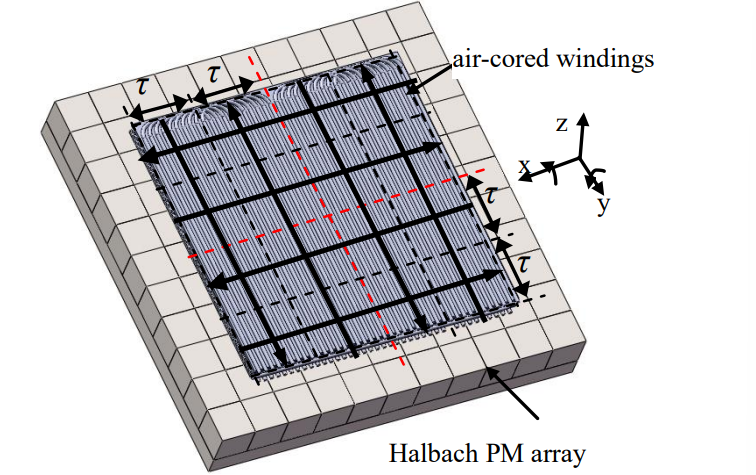
\includegraphics[width=0.5\textwidth]{Multilayer_Mover_Coil}}
%\hspace{2mm}
\subfloat[استفاده از سیم‌پیچ‌های یک لایه متعامد
\cite{RN14}]
{ \label{fig:Single_layer_Mover_Coil}
\includegraphics[width=0.5\textwidth]{Single_layer_Mover_Coil}}%
\caption{ساختار سیستم‌های MLPM با سیم‌پیچ‌های متحرک و آهنربای ثابت}
\label{fig:Moveing_Coil} %% label for entire figure
\end{figure}

با وجود اینکه این معماری امکان دستیابی به شناوری پایدار و حرکت با شش درجه آزادی را فراهم می‌کند، اما در کاربردهای عملی با محدودیت‌هایی مواجه است که بر عملکرد نهایی سیستم تأثیرگذار هستند. نخستین محدودیت، نیاز به تأمین انرژی الکتریکی برای سیم‌پیچ‌ها از طریق سیم‌های فیزیکی است که این امر به‌طور اجتناب‌ناپذیری ارتباط فیزیکی میان جسم متحرک و محیط اطراف را برقرار می‌سازد، در نتیجه حرکت آزادانه کامل جسم متحرک محدود می‌شود. دومین محدودیت، چالش خنک‌کاری سیم‌پیچ‌ها است که به دلیل ماهیت متحرک و معلق بودن آن‌ها، اجرای یک سیستم خنک‌کننده کارآمد دشوار خواهد بود. این مشکلات، نیاز به ارائه معماری جدیدی را آشکار می‌کند که بتواند این چالش‌ها را برطرف سازد.

\subsection{‌آهنرباهای متحرک و سیم‌پیچ‌های ثابت}

معماری دیگری که برای طراحی دستگاه‌های MLPM ارائه شده است، شامل قرار دادن سیم‌پیچ‌ها در بخش استاتور و استفاده از آهنرباهای دائمی در بخش متحرک می‌باشد. این ساختار نوین که در بسیاری از پژوهش‌ها مورد استفاده قرار گرفته، مشکلات معماری‌های پیشین مانند محدودیت جابه‌جایی متحرک ناشی از اتصالات فیزیکی و چالش‌های خنک‌کاری سیم‌پیچ‌ها را برطرف کرده و منجر به بهبود عملکرد کلی سیستم شده است.

در پژوهش 
\cite{RN7}
 استاتوری با چینش سیم‌پیچ‌ها مطابق با الگوی شاه‌ماهی
\LTRfootnote{Herringbone pattern}
 طراحی و پیاده‌سازی شده است. این طراحی امکان اعمال نیروی مغناطیسی به دو آهنربای دیسکی تعبیه‌شده در بخش متحرک را فراهم کرده است که دقتی در حدود 1 درجه در زوایای حرکت و 1 میلی‌متر در موقعیت متحرک به دست آورده است
\cite{RN7}
. در ادامه این پژوهش، ساختاری جدید برای بخش متحرک ارائه شده که شامل 6 آهنربای دیسکی با چینش کروی و فواصل ثابت می‌باشد. این طراحی توانسته است چرخش آزادانه متحرک را حول سه محور ممکن سازد 
\cite{RN39}.
شکل (
\ref{fig:Moving_Magnet_1})
همچنین در پژوهش 
\cite{RN62}
 نیز از این چینش سیم‌پیچ‌ها استفاده شده و مطابق با شبیه‌سازی‌های ارائه شده، مزیت آنان در ایجاد میدان مغناطیسی یکنواخت‌تر در نواحی کناری سیم‌پیچ‌ها نمایش داده شده است.

استفاده از سیم‌پیچ‌های سه‌فاز به‌جای تغذیه با جریان مستقیم، رویکردی است که در پژوهش 
\cite{RN24}
معرفی و اجرا شده است. در این ساختار، چهار آرایه از سیم‌پیچ‌های سه‌فاز، همان‌طور که در 
شکل (
\ref{fig:Moving_Magnet_2})
 نشان داده شده است، به‌گونه‌ای طراحی شده‌اند که نیروی مغناطیسی لازم را تولید کنند.

به ‌منظور کاهش هزینه‌ی محاسباتی در جابه‌جایی‌های طولانی، پژوهش 
\cite{RN32}
 ساختاری را ارائه کرده است که از دو مجموعه سیم‌پیچ‌ سه‌فاز و تک‌فاز تشکیل شده است. در این طراحی، کنترل حرکت در مسافت‌های طولانی توسط سیم‌پیچ‌های سه‌فاز انجام می‌پذیرد، در حالی که برای تنظیم دقیق موقعیت متحرک در صفحه، از سیم‌پیچ‌های تک‌فاز بهره برده می‌شود.
شکل (
\ref{fig:Moving_Magnet_3})

استفاده از سیم‌پیچ‌های ماژولار در طراحی استاتورهایی با چینش دوبعدی، رویکردی است که در دستگاه‌های MagTable و MagFloor از دانشگاه واترلو پیاده‌سازی شده است
\cite{RN8,RN30,RN10}
 در این طراحی، ماژول‌هایی از سیم‌پیچ‌های با سطح مقطع مربع به‌گونه‌ای طراحی شده‌اند که با قرار گرفتن در کنار یکدیگر، فضای کاری نامحدودی برای جابه‌جایی متحرک فراهم می‌کنند.(شکل
\ref{fig:Moving_Magnet_4})
 همچنین، پژوهش
\cite{RN8}
 نشان داده است که آهنرباهای با سطح مقطع مربع، در مقایسه با سیم‌پیچ‌های دایروی با جریان الکتریکی مشابه، می‌توانند شدت میدان مغناطیسی بیشتری ایجاد کنند، که این مزیت عملکرد کلی سیستم را بهبود می‌بخشد.

\begin{figure}[ht]
\centering 
\subfloat[الگوی شاه‌ماهی سیم‌پیچ‌ها
\cite{RN39}]
{ \label{fig:Moving_Magnet_1}
\includegraphics[width=0.45\textwidth]{Moving_Magnet_1}}
\hspace{2mm}
\subfloat[سیم‌پیچ‌های سه فاز
\cite{RN24}]
{ \label{fig:Moving_Magnet_2}
\includegraphics[width=0.45\textwidth]{Moving_Magnet_2}}
\\ % Newline to wrap the figures to the next row
\subfloat[ساختار دوگانه سیم‌پیچ‌ها
\cite{RN32}]
{ \label{fig:Moving_Magnet_3}
\includegraphics[width=0.45\textwidth]{Moving_Magnet_3}}
\hspace{2mm}
\subfloat[ساختار ماژولار سیم‌پیچ‌ها
\cite{RN10}]
{ \label{fig:Moving_Magnet_4}
\includegraphics[width=0.45\textwidth]{Moving_Magnet_4}}
\label{fig:Moveing_Magnet} %% label for entire figure
\caption{ساختارهای آهنرباهای متحرک و سیم‌پیچ‌های ثابت}
\end{figure}








\section{ساختار آهنرباهای دائمی}

همان‌طور که در بخش قبل اشاره شد، میدان مغناطیسی کنترل‌شده توسط آهنرباهای الکتریکی ایجاد می‌شود و بر اثر تعامل این میدان متغیر با میدان ثابت آهنرباهای دائمی، نیرویی بر بخش متحرک دستگاه وارد می‌شود که حرکت آن را در راستاهای مختلف ممکن می‌سازد. بنابراین، طراحی بهینه آهنرباهای دائمی، به‌ویژه برای تولید میدان مغناطیسی قوی‌تر با کمترین وزن، در بهبود کارایی دستگاه نقش کلیدی دارد. در این بخش، طراحی‌های مختلف آهنرباهای دائمی که در پژوهش‌های پیشین ارائه شده‌اند، با تمرکز بر بهینه‌سازی این ویژگی‌ها بررسی می‌شوند.
\subsection{استفاده از آهنرباهای دیسکی}

استفاده از آهنرباهای دیسکی رویکردی ساده و مؤثر برای ایجاد میدان مغناطیسی دائمی محسوب می‌شود. با انتخاب موادی با خاصیت مغناطیسی بالا، مانند آهنرباهای نئودیمیومی، می‌توان به شدت میدان مغناطیسی مطلوب دست یافت. به عنوان نمونه، در پژوهش 
\cite{RN7}
 از دو آهنربای دیسکی جهت تأمین میدان مغناطیسی ثابت استفاده شده است. همچنین در پژوهش 
\cite{RN39}
 با به‌کارگیری ۶ آهنربای دیسکی، امکان چرخش آزادانه حول سه محور فراهم شده است.(شکل
\ref{fig:Disk_Magnet_1})
 در پژوهش 
\cite{RN8}
 نیز از ترکیب‌های متفاوتی از آهنرباهای دیسکی برای بخش متحرک دستگاه استفاده شده است، که این ترکیب‌ها شامل تغییر اندازه‌ی یک آهنربا و استفاده از سه آهنربای دیسکی است. سیستم شناوری مغناطیسی با پنج درجه آزادی که تنها از یک آهنربای دیسکی تشکیل شده است، در پژوهش 
\cite{RN62}
 به عنوان نمونه‌ای موفق از این رویکرد معرفی شده است. این طراحی، با وجود سادگی معماری، توانسته نتایج رضایت‌بخشی را از نظر عملکرد ارائه دهد و نشان می‌دهد که استفاده از آهنربای دیسکی، علاوه بر سادگی، می‌تواند در کاربردهای مختلف به‌ویژه در سیستم‌های با نیاز به دقت بالا و چند درجه آزادی، کارآمد باشد. شکل((
\ref{fig:Disk_Magnet_2})


\begin{figure}[ht]
\centering 
\subfloat[دو آهنربای دیسکی
\cite{RN7}]
{ \label{fig:Disk_Magnet_1}
\includegraphics[width=0.5\textwidth]{Disk_Magnet_1}}
%\hspace{2mm}
\subfloat[یک آهنربای دیسکی
\cite{RN62}]
{ \label{fig:Disk_Magnet_2}
\includegraphics[width=0.5\textwidth]{Disk_Magnet_2}}%
\caption{استفاده از آهنربای دیسکی در طراحی متحرک}
\label{fig:Disk_Magnet} %% label for entire figure
\end{figure}



\subsection{آرایه‌ی هالباخ یک بعدی}

آرایه‌ی هالباخ
\LTRfootnote{Halbach Array}
 به‌عنوان چینشی از آهنرباهای دائمی تعریف می‌شود که در آن جهت مغناطیس‌شوندگی هر آهنربا با آهنربای مجاور خود ۹۰ درجه تفاوت دارد. این آرایه به‌طور خاص قادر است میدان مغناطیسی در یک سوی آرایه را خنثی کرده و در سوی دیگر میدان را به میزان تقریبی 1.4 برابر افزایش دهد.
مزیت این ساختار در طراحی سیستم‌های MLPM، توانایی آن در تولید شدت میدان مغناطیسی بیشتر است. به‌همین‌دلیل، این چینش در بسیاری از پژوهش‌ها مورد استفاده قرار گرفته است.
با این حال، استفاده از تنها یک آرایه‌ی یک‌بعدی هالباخ به‌تنهایی نمی‌تواند نیرویی در دو راستای افقی ایجاد کند. لذا معمولاً از تعداد بیشتری از این آرایه‌ها در ساختار متحرک استفاده می‌شود. به‌عنوان مثال، در پژوهش‌های 
\cite{RN24,RN27}
 از چهار آرایه‌ی هالباخ یک‌بعدی در بخش متحرک استفاده شده است که هر یک از این آرایه‌ها قادر به ایجاد نیرویی در یکی از راستاهای افقی و عمودی هستند.
در پژوهش 
\cite{RN39}
، مشابه آنچه که در بخش استاتور پیاده‌سازی شده بود، از ساختار دوگانه‌ای در بخش متحرک بهره‌برداری شده است، به‌گونه‌ای که دو مجموعه چهارگانه از آرایه‌های هالباخ در معماری این بخش به‌کار رفته‌اند.

\begin{figure}[ht]
\centering 
\subfloat[آرایه‌ی هالباخ
\cite{RN16}]
{ \label{fig:halbach1D}
\includegraphics[width=0.5\textwidth]{halbach1D}}
%\hspace{2mm}
\subfloat[4 آرایه‌ی یک بعدی هالباخ
\cite{RN39}]
{ \label{fig:4_halbach1D_array}
\includegraphics[width=0.5\textwidth]{4_halbach1D_array}}%
\caption{آرایه هالباخ یک‌بعدی}
\label{fig:halbach1D} %% label for entire figure
\end{figure}

\subsection{آرایه هالباخ دوبعدی}

برای رفع محدودیت‌های آرایه‌ی هالباخ یک‌بعدی که تنها در یک راستا نیرو ایجاد می‌کند، ساختار جدیدی از آرایه‌ی دوبعدی ارائه شده است. این آرایه قادر است میدان مغناطیسی را در یک طرف صفحه حذف و در طرف دیگر تقویت کند. با این ویژگی، استفاده از چندین آرایه برای تأمین میدان مغناطیسی ثابت ضروری نخواهد بود. طراحی آرایه‌ی دوبعدی در بسیاری از پژوهش‌ها برای بخش‌های متحرک یا استاتور سیستم‌های MLPM به کار گرفته شده است.

استفاده از آرایه‌ی هالباخ در پژوهش‌های مختلفی از جمله
\cite{RN10, RN30} 
و
\cite{RN55, RN26} 
نشان‌دهنده‌ی عملکرد بهینه‌ی این معماری در بخش متحرک سیستم‌های MLPM است.(شکل
\ref{fig:halbach2D_2})
 همچنین در پژوهش
\cite{RN14}
 از این آرایه به عنوان بخشی از استاتور دستگاه بهره‌گیری شده است. در 
\cite{RN61}
 ماژول‌هایی برای ساخت این آرایه استفاده شده (شکل
\ref{fig:halbach2D_4})
 و در
\cite{RN49}
 برای تشکیل آرایه از قطعات آهنی در فضای خالی میان آن استفاده شده است؛ اما این رویکرد باعث ایجاد خطا در دقت میدان مغناطیسی شده است. (شکل
\ref{fig:halbach2D_3})
علاوه بر این، در پژوهش
\cite{RN28}
، طراحی جدیدی با آهنرباهایی با میزان مغناطیس‌شوندگی و ارتفاع متفاوت پیشنهاد شده است.
\begin{figure}[ht]
\centering 
\subfloat[آرایه هالباخ دو بعدی و میدان مغناطیسی آن
\cite{RN10}]
{ \label{fig:halbach2D_2}
\includegraphics[width=0.45\textwidth]{halbach2D_2}}
\hspace{2mm}
\subfloat[آرایه هالباخ دوبعدی با قطعات آهنی در فضاهای خالی
\cite{RN49}]
{ \label{fig:halbach2D_3}
\includegraphics[width=0.45\textwidth]{halbach2D_3}}
\\ % Newline to wrap the figures to the next row
\subfloat[آرایه هالباخ دوبعدی ماژولار
\cite{RN61}]
{ \label{fig:halbach2D_4}
\includegraphics[width=0.45\textwidth]{halbach2D_4}}
\caption{آرایه هالباخ دو‌بعدی}
\label{fig:halbach2D} %% label for entire figure

\end{figure}
\section{طراحی کنترلر}
همان‌طور که پیش‌تر اشاره شد، سیستم‌های شناوری مغناطیسی ذاتاً ناپایدار هستند و برای دستیابی به پایداری، به کنترلری با عملکرد دقیق و خطای کم نیاز است. در پژوهش‌های مختلف، از کنترلرهای گوناگونی برای این سیستم‌ها بهره گرفته شده است؛ از جمله کنترلرهای کلاسیک نظیر PID، کنترلرهای مدرن مانند کنترل مبتنی بر پیش‌بینی مدل (MPC) و همچنین مدل‌های مبتنی بر هوش مصنوعی نظیر شبکه‌های بازگشتی GRU. در این بخش، به بررسی این کنترلرها و مقایسه‌ عملکرد آنها خواهیم پرداخت.
\subsection{کنترلر PID}

کنترل تناسبی-انتگرالی-مشتقی (PID) به عنوان یکی از پرکاربردترین و موثرترین کنترلرهای کلاسیک در سیستم‌های دینامیکی، گزینه‌ای مناسب برای کنترل سیستم‌های MLPM محسوب می‌شود. این کنترلر به دلیل سادگی در پیاده‌سازی، تنظیم دقیق و توانایی تنظیم خروجی سیستم بر اساس خطاهای ورودی، به‌طور گسترده در سیستم‌های مختلف استفاده شده است. برای کنترل سیستم‌های MLPM، به ازای هر درجه آزادی یک کنترلر PID طراحی و پیاده‌سازی می‌شود تا بتواند جریان الکتریکی سیم‌پیچ‌ها را تنظیم کرده و میدان مغناطیسی لازم برای ایجاد و حفظ موقعیت متحرک را تأمین کند.

در پژوهش‌های متعددی از کنترلر PID برای سیستم‌های MLPM بهره گرفته شده است. به عنوان مثال، در 
\cite{RN39,RN24}
از کنترلرهای PID ساده برای کنترل جریان سیم‌پیچ‌ها استفاده شده که وظیفه تنظیم میدان مغناطیسی و در نتیجه، کنترل موقعیت جسم متحرک را بر عهده دارند. علاوه بر این، در پژوهش
\cite{RN32}
، از دو کنترلر PID در یک ساختار دوگانه استفاده شده است. کنترلر اول برای جابه‌جایی‌های بلند و در مسافت‌های طولانی به کار رفته و جریان سیم‌پیچ‌های اصلی را تنظیم می‌کند، در حالی که کنترلر دوم برای حرکات دقیق کوتاه‌برد طراحی شده و کنترل جریان سیم‌پیچ‌های ثانویه را بر عهده دارد. این روش باعث بهینه‌سازی کنترل دقیق و بهبود دقت در حرکات کوتاه‌برد و جابه‌جایی‌های سریع می‌شود.
همچنین در سیستم MagTable، برای کنترل دقیق موقعیت آهنرباهای دائمی، از شش کنترلر PID به‌صورت همزمان استفاده شده است تا نیروی متوازن برای پایدارسازی موقعیت متحرک در چندین جهت فراهم شود 
\cite{RN8}
. این نوع طراحی و استفاده از کنترلرهای PID نشان می‌دهد که علی‌رغم محدودیت‌های موجود در کنترلرهای کلاسیک، این روش همچنان در بسیاری از سیستم‌های مغناطیسی پیچیده مانند MLPM کارایی بالایی دارد.

\begin{figure}[ht]
\centering{\includegraphics[width=0.5\textwidth]{PID_1}}
\caption{کنترلر PID با 6 درجه آزادی
\cite{RN8}}
\label{fig:PID}
\end{figure}


\subsection{کنترلر مبتنی بر پیش‌بینی مدل MPC}
برای کنترل سیستم‌های MLPM اگر مدل سیستم به روش‌های تحلیلی و یا عددی به دست آمده و تخمین زده شده باشد، می‌توان از این مدل‌ها برای طراحی کنترلرهای پیشرفته‌تر با هدف پیش‌بینی رفتار سیستم و استفاده از آن به صورت پیش‌خور در حلقه‌ی کنترلی استفاده کرد. روش‌های تخمین مدل این سیستم‌ها در بخش‌های بعد مورد بررسی قرار می‌گیرد. در این بخش، کنترلرهای ارائه شده در پژوهش‌های دیگر ارائه می‌شود.
به دست آوردن معادلات دینامیکی سیستم و استفاده از آنها در پیش‌بینی روشی تحلیلی است که در 
\cite{RN55}
 استفاده شده است و مدل کنترلی متشکل از بلوک‌های پس‌خور و پیش‌خور برای کنترل موقعیت آهنربا طراحی شده است. همچنین در 
\cite{RN62}
 از یک جدول جستجو برای تعیین رفتار سیستم در نقاط مختلف فضا استفاده شده است که این جدول به عنوان پیش‌خور به مدل کنترلی داده می‌شود. در ادامه‌ی این پژوهش، با استفاده از روش‌های شناسایی سیستم، مدلی تقریبی برای رفتار سیستم در نظر گرفته شده است و با استفاده از این مدل برای پیش‌بینی رفتار سیستم‌ مدل MPC پیاده‌سازی شده است. پژوهش 
\cite{RN30}
 با تمرکز بر ارائه‌ی یک مدل پیش‌بین، با استفاده از معادلات دینامیکی سیستم و همچنین روش‌پیش‌بینی حالت بی‌تاخیر، رفتار آینده‌ی سیستم را محاسبه می‌کند.
\begin{figure}[ht]
\centering 
\subfloat[\cite{RN55}]{
    \label{fig:MPC_1}
    \includegraphics[width=0.45\textwidth]{MPC_1}}
%\hspace{2mm}
\subfloat[\cite{RN62}]{
    \label{fig:MPC_2}
    \includegraphics[width=0.45\textwidth]{MPC_2}}
\\ % Newline to wrap the figures to the next row
\subfloat[\cite{RN61}]{
    \label{fig:MPC_3}
    \includegraphics[width=0.45\textwidth]{MPC_3}}
\subfloat[\cite{RN61}]{
    \label{fig:MPC_4}
    \includegraphics[width=0.45\textwidth]{MPC_4}}
\caption{کنترلر MPC}
\label{fig:MPC} %% label for entire figure
\end{figure}

\FloatBarrier

\subsection{کنترلر مبتنی بر هوش مصنوعی}

یکی از روش‌های نوین برای پیش‌بینی رفتار سیستم‌های پیچیده مانند MLPM، استفاده از مدل‌های هوش مصنوعی به‌ویژه شبکه‌های عصبی بازگشتی (RNN) است. این مدل‌ها با یادگیری دینامیک سیستم و ارتباط بین ورودی‌ها و خروجی‌ها، می‌توانند به‌طور مؤثری رفتار سیستم را در شرایط مختلف پیش‌بینی کنند. در این راستا، پژوهش
\cite{RN61}
از یک مدل بازگشتی GRU 
\LTRfootnote{Gated Recurrent Unit}
 استفاده کرده است. این مدل بر اساس داده‌های جمع‌آوری‌شده از عملکرد دستگاه MLPM آموزش دیده و توانسته است با دقت بالا تغییرات دینامیکی سیستم و پاسخ آن به ورودی‌های گوناگون را پیش‌بینی کند. استفاده از GRU به دلیل توانایی آن در مدل‌سازی وابستگی‌های زمانی و در نظر گرفتن اطلاعات قبلی برای پیش‌بینی‌های دقیق‌تر، رویکردی مناسب در این پژوهش بوده است.(شکل 
\ref{fig:GRU}

\begin{figure}[ht]
\centering
\includegraphics[width=0.5\textwidth]{GRU_1}
\caption{کنترلر پیش‌خور GRU \cite{RN61}}
\label{fig:GRU}
\end{figure}

\section{مدل‌سازی و تخمین سیستم}
در روش بار نقطه‌ای برای تحلیل میدان مغناطیسی، فرض می‌شود که توزیع بار مغناطیسی در یک حجم به‌صورت متمرکز در هشت نقطه در گوشه‌های آن حجم قرار گرفته است. با این فرض، اثر مغناطیسی این جسم می‌تواند به‌صورت مجموع آثار هر یک از بارهای نقطه‌ای محاسبه شود. این رویکرد امکان محاسبه‌ی دقیق شدت میدان مغناطیسی و نیروی وارد بر یک جسم خارجی را فراهم می‌آورد. از طریق محاسبه‌ی میدان‌های ناشی از هر بار نقطه‌ای و جمع آنها، میدان مغناطیسی کل حاصل می‌شود و به این ترتیب، شدت میدان مغناطیسی ناشی از آهنربای دائمی به کمک این روش به‌طور دقیق محاسبه می‌گردد. در ادامه، معادلات مربوط به محاسبه‌ی شدت میدان مغناطیسی ارائه شده‌اند.
\subsection{مدل بار مغناطیسی سطحی}
در این مدل، فرض بر این است که بار مغناطیسی در یک المان حجم سه‌بعدی به‌صورت توزیعی از بارهای مغناطیسی با چگالی بار J بر روی دو صفحه‌ی موازی قرار گرفته است. با استفاده از این فرض، میدان مغناطیسی ایجادشده توسط این حجم به‌صورت میدان حاصل از توزیع بارهای مغناطیسی محاسبه می‌شود. این مدل امکان تحلیل دقیق‌تر رفتار میدان مغناطیسی را فراهم می‌کند. مقایسه نتایج حاصل از این مدل با شبیه‌سازی المان محدود
\LTRfootnote{Finite Element Method (FEM)}
 در پژوهش
\cite{RN44}
نشان داده است که این روش مدل‌سازی برای سیستم‌های MLPM دقت و کارایی بالایی دارد.

\begin{figure}[ht]
\centering
\includegraphics[width=0.5\textwidth]{Magnetic surface charge_2}
\caption{مدل بار مغناطیسی سطحی \cite{RN44}}
\label{fig:Magnetic surface charge}
\end{figure}

\subsection{مدل بار مغناطیسی نقطه‌ای}
در روش بار نقطه‌ای برای تحلیل میدان مغناطیسی، فرض می‌شود که توزیع بار مغناطیسی در یک حجم به‌صورت متمرکز در هشت نقطه در گوشه‌های آن حجم قرار گرفته است. با این فرض، اثر مغناطیسی این جسم می‌تواند به‌صورت مجموع آثار هر یک از بارهای نقطه‌ای محاسبه شود. این رویکرد امکان محاسبه‌ی دقیق شدت میدان مغناطیسی و نیروی وارد بر یک جسم خارجی را فراهم می‌آورد. از طریق محاسبه‌ی میدان‌های ناشی از هر بار نقطه‌ای و جمع آنها، میدان مغناطیسی کل حاصل می‌شود و به این ترتیب، شدت میدان مغناطیسی ناشی از آهنربای دائمی به کمک این روش به‌طور دقیق محاسبه می‌گردد. در ادامه، معادلات مربوط به محاسبه‌ی شدت میدان مغناطیسی ناشی از هر بار نقطه‌ای ارائه شده‌است.
\begin{align}
B_{xk} &= \frac{\epsilon_k}{4\pi} \ln\left(-y_r + \sqrt{x_r^2 + y_r^2 + z_r^2}\right), \\
B_{yk} &= \frac{\epsilon_k}{4\pi} \ln\left(-x_r + \sqrt{x_r^2 + y_r^2 + z_r^2}\right), \\
B_{zk} &= \frac{\epsilon_k}{4\pi} \arctan\left( \frac{x_r y_r}{\sqrt{x_r^2 + y_r^2 + z_r^2}} \right),
\end{align}

\begin{figure}[ht]
\centering
\includegraphics[width=0.5\textwidth]{Magnetic_Node}
\caption{مدل بار مغناطیسی نقطه‌ای \cite{RN44}}
\label{figMagnetic_Node}
\end{figure}

\subsection{مدل های مبتنی بر داده}

در این روش‌ها، به‌جای مدل‌سازی دقیق ساختار فیزیکی دستگاه و استخراج معادلات دینامیکی آن، پارامترهای مورد نیاز مانند شدت میدان مغناطیسی از طریق داده‌های تجربی یا شبیه‌سازی المان محدود (FEM) تخمین زده می‌شوند. این رویکرد مبتنی بر داده نیازمند دسترسی به اطلاعات دقیق از سیستم واقعی یا شبیه‌سازی کامل آن است تا بتوان دقت و اعتبار تخمین‌ها را ارزیابی کرد. در پژوهش 
\cite{RN10}
، برای تخمین شدت میدان مغناطیسی آرایه هالباخ دوبعدی از معادلات هارمونیک و سری فوریه استفاده شده است. تغییرات میدان مغناطیسی تولیدشده توسط این آرایه به‌صورت موجی سینوسی مدل‌سازی شده است، اما این روش تنها زمانی دقیق است که فرض شود سطح آرایه به‌صورت نامحدود ادامه دارد. برای حل این مشکل، آرایه به سه ناحیه مرکزی، کناری و گوشه‌ای تقسیم‌بندی شده و برای هر ناحیه هارمونیک‌های مجزا در نظر گرفته شده است. نتایج این پژوهش نشان می‌دهند که با استفاده از سه هارمونیک اول، می‌توان میدان مغناطیسی را در نواحی کناری و گوشه‌ای با دقت مناسبی تخمین زد.

\begin{figure}[ht]
\centering 
\subfloat[\cite{RN10}]{
\label{fig:harmonic_1}
\includegraphics[width=0.45\textwidth]{harmonic_1}}
\hspace{2mm}
\subfloat[\cite{RN10}]{
\label{fig:harmonic_2}
\includegraphics[width=0.45\textwidth]{harmonic_2}}
\caption{مدل هارمونیک}
\label{fig:harmonic}
\end{figure}



!
	را در فایل 
	\lr{main.tex}،
	غیرفعال%
	\footnote{
		برای غیرفعال کردن یک دستور، کافی است در ابتدای آن، علامت درصد انگلیسی (\%) بگذارید.
	}
	کنید. در غیر این صورت، ابتدا مطالب دو فصل اول پردازش شده و سپس مطالب فصل ۳ پردازش می‌شود که این کار باعث طولانی شدن زمان پردازش می‌گردد. هر زمان که خروجی کل \پ را خواستید، تمام فصل‌ها را دوباره در
	\lr{main.tex}
	فعال نمائید.
	بدیهتاً لازم نیست فصل‌های \پ را به ترتیب تایپ کنید. مثلاً می‌توانید ابتدا مطالب فصل ۳ را تایپ نموده و سپس مطالب فصل ۱ را تایپ کنید. 
	
	\subsubsection{مراجع}
	برای وارد کردن مراجع \پ کافی است فایل 
	\lr{MyReferences.bib}
	را باز کرده و مراجع خود را به شکل اقلام نمونهٔ داخل آن، وارد کنید.  سپس از \lr{bibtex} برای تولید مراجع با قالب مناسب استفاده نمائید. برای توضیحات بیشتر بخش \ref{Sec:Ref} از پیوست \ref{app:latexIntro} و نیز پیوست \ref{app:refMan} را ببینید.
	
	\subsubsection{واژه‌نامه فارسی به انگلیسی و برعکس}
	برای وارد کردن معادل فارسی اصطلاحات لاتین در متن و تهیه فهرست واژه‌نامه از آنها، از بستهٔ
	\lr{glossaries}
	و نرم‌افزار
	\lr{xindy}
	استفاده می‌شود. بدین منظور کافی است اصطلاحات لاتین و ترجمهٔ آنها را در فایل
	\lr{words.tex}
	وارد کرده و هر جای متن که خواستید با دستورات
	\verb|gls{label}|
	یا \verb|glspl{label}|
	معادل فارسی مفرد یا جمع یک اصطلاح را بیاورید.
	
	مثلا در اینجا، واژهٔ
	«\gls{Action}»
	برای بار اول و دوباره
	«\gls{Action}»
	برای بار دوم در متن ظاهر شده است.
	جهت توضیحات بیشتر به پیوست
	\ref{app:refMan}
	مراجعه کنید.
	برای ایجاد واژه نامه باید دستورات زیر را اجرا کنید:\\
	{\small
	\begin{LTR}
		\begin{verbatim}
			xindy -L persian-variant3 -C utf8 -I xindy -M %.xdy -t %.glg -o %.gls %.glo
			xindy -L persian-variant3 -C utf8 -I xindy -M %.xdy -t %.blg -o %.bls %.blo
			xindy -L english -C utf8 -I xindy -M %.xdy -t %.alg -o %.acr %.acn
		\end{verbatim}
	\end{LTR}}

	
	\subsubsection{نمایه}
	برای وارد کردن نمایه، باید از 
	\lr{xindy}
	استفاده کنید. 
	برای وارد کردن نمایه باید از دستور
	\verb*|\index{lable}|
	\index{نمایه}
	استفاده کنید. مثال‌ها بیشتر در پیوست
	\ref{app:latexIntro}
	قسمت 
	\ref{app:index}
	آورده شده است. برای ساختن نمایه‌ها با استفاده از 
	\lr{xindy}
	ابتدا باید فایل 
	\lr{main.tex}
	را اجرا کنید و سپس با دستور:
	{\small
		\begin{LTR}
			\begin{verbatim}
				xindy -M texindy -C utf8 -L persian-variant2 %.idx
			\end{verbatim}
	\end{LTR}}
    نمایه را ایجاد کنید و دوباره  فایل 
	\lr{main.tex}
	را اجرا کنید. ممکن است پس از ایجاد نمایه‌ی جدید و یا حذف نمایه‌های قبلی نیاز باشد 
	جند مرتبه این سه مرحله را تکرار کنید تا نمایه به صورت کامل تصحیح شود.


\subsection{اگر سوالی داشتم، از کی بپرسم؟}
می‌توان گفت که پاسخ اغلب سوالات را می‌توانید با یک جست و جوی ساده در اینترنت پیدا کنید. اگر به هنگام اجرا با خطایی مواجه شدید متن خطا را در 
\lr{google}
وارد جست و جو نمایید. همچنین می‌توانید سوالات خود را در 
\lr{\href{https://tex.stackexchange.com/}{stackexchange}}
یا
\href{http://qa.parsilatex.com}{سایت پرسش و پاسخ پارسی‌لاتک}%
\LTRfootnote{http://qa.parsilatex.com}
مطرح نمایید.
یا به
\href{http://forum.parsilatex.com}{بایگانی تالارگفتگوی قدیمی پارسی‌لاتک}%
\LTRfootnote{http://forum.parsilatex.com}
مراجعه کنید.
همچنین در صورت بافتن مشکلی در قالب می‌توانید در بخش مشکلات گیت‌هاب پروژه به آدرس 
\lr{\href{https://github.com/msinamsina/kntu-thesis/issues}{https://github.com/msinamsina/kntu-thesis/issues}}
آن را مطرح نمایید.

\section{محتویات فصل اول یک پایان‌نامه}
در فصل اول از \پ به بیان مقدمه پرداخته می‌شود.
هدف از فصل مقدمه%
\LTRfootnote{Introduction}،
شرح مختصر مسأله به منظوری روشن شدن هدف تحقیق و بیان اهمیت و انگیزه‌ی محقق از پرداختن به موضوع \پ است. همچنین در این فصل باید اشاره‌ی کوتاه‌ی به روش و مراحل تحقیق شود تا یه صورت کلی زمینه‌های اطلاعاتی لازم را برای خواننده فراهم شود. بیان دقیق و کامل صورت مساله در این فصل اهمیت بالایی دارد و موجب می‌شود خواننده بهتر به اهمیت کار شما پی‌ببرد و او را به خواندن ادامه‌ی مطالب ترغیب می‌کند. در مقدمه لازم است به کمک سوابق تحقیق و اطلاعات موجود (با ذکر منبع) خلاهای موجود در زمینه تحقیق نشان داده شود و با روشی منظم، منطقی و هدف‌دار،  به درک بیشتر خواننده از راه حل ارائه شده برای رفع این خلاها کمک کرد. مقدمه مناسب‌ترین جا برای ارائهٔ اختصارات و بعضی توضیحات کلی است، توضیحاتی که شاید نتوان در مباحث دیگر آنها را شرح داد. 
مقدمه، یکی از ارکان اساسی و اصلی پایان نامه است که مهمترین قسمت‌های آن در ادامه آمده است، اما باید به این نکته توجه شود که بهتر است عناوین این قسمت‌ها بسته به موضوع تحقیق  تغییر کنند و از عناوین مناسب برای این کار استفاده گردد و همچنین به بنابر سلیقه‌ی نگارنده و با مشورت استاد راهنما برخی از این قسمت‌ها می‌توانند با هم ترکیب شوند و یک قسمت را تشکبل دهند.

\subsection{عنوان تحقیق} 
در این بخش باید به طور مختصر عنوان و زمینه‌ی تحقیق خود و علت به وجود آمدن آن را شرح دهید.
از توضیحات جزئی در این قسمت پرهیز شود و تلاش شود مطالب به دور از پیچیدگی و ابهام بیان گردد.
\subsection{تعریف مسأله }
وظیفه اصلی مقدمه بیان چرایی و علت انجام تحقیق در مورد موضوع محوری \پ است. در این بخش مساله‌ای که قرار است به آن پاسخ دهید را به طور دقیق شرح دهید. اگر مساله مورد نظر شما در زمینه‌ای جدید مطرح شده است، از زمینه‌های مشابه و نزدیک برای توضیح مساله کمک بگیرید تا خواننده دقیقا متوجه خروجی مورد نظر شما در این تحقیق شود و به طور کلی پرسش‌های اساسی و که در این تحقیق قصد پاسخ به آن را دارید را در ذهن خواننده ایجاد نمایید. گاهی می‌توانید ابتدا اهمیت موضوع را بیان و سپس پرسش خود را در آن موضوع مطرح کنید.

\subsection{تاریخچه‌ای از موضوع تحقیق}
به طور کلی پیش از ورود به موضوع هر تحقیقی باید به مطالعه‌ی کار های پیشین صورت گرفته در موضوع تحقیق و یا موضوعات نزدیک به آن پرداخته شود تا خلاهای موچود مشخص گردد و میزان نوآوری محقق در تحقیق پیش رو مشخص گردد. اما در بیان تاریخچه نباید زیاده‌روی کرد. بهتر است بیشتر به مقالات دو سال قبل از کارتان اشاره شود اما گاهی نیاز است به برخی مقالات قدیدمی‌تر نیز که پایه‌ای برای ایده های محوری مقالات اخیر است نیز اشاره‌ شود. فصل دوم تحقیق عموما به مروری بر ادبیات موضوع می‌پردازد بنابراین یا باید این قست خیلی مختصر باشد و مطالب تکراری در فصل دوم بیان نگردد و یا فصل دوم را به موضوع دیگری اختصاص دهید و در این بخش به تفصیل به مروری بر ادبیات موضوع بپردازید. در انتهای این بخش می‌توانید به کمک چند جدول و نمودار کارهای پیشین را در یک نگاه با یکدیگر مقایسه کنید که این کار دید بهتری به خواننده می‌دهد و می‌توان به کمک آن خلاهای موجود را برجسته نمود.

\subsection{تعریف موضوع تحقیق}
در این قسمت محقق، به  تفصیل موضوع تحقیق و یا نیاز احساس در حوزه تحقیق بیان می‌گردد و فرضیات مساله  مشخص می‌شود.

\subsection{هدف یا هدف‌های کلی، نوآوری و اهمیت  تحقیق}
این قسمت باید با جملات مثبت و کلی دستاورد‌هایی که این تحقیق دارد و کمکی که به تحیقات آتی می‌کند را شرح دهید. همچنین نوآوری‌ها و دستاوردهای علمی و عملی به دست آمده در این پژوهش را نیز بجسته کنید تا خواننده متوجه شود در این \پ به جه نتیجه‌ای خواهید رسید.

\subsection{روش انجام تحقیق}
در این قسمت، پژوهشگر روش‌های مختلفی که برای گردآوری مطالب خود بکار برده، ذکر می‌کند. به عنوان مثال روش‌های جمع‌آوری داده و به کمک آزمایش‌ها مختلف را بیان می‌کند. این قسمت نیز باید مختصر بیان شود و نمای کلی راه طی شده در تحقیق را نشان دهد.

\subsection{تعریف واژه‌ها (اختیاری)}
در این قسمت محقق باید واژه‌هایی را که ممکن است برای خواننده آشنا نباشد، تعریف کند.

\subsection{خلاصه فصل‌ها}
در آخرین قسمتِ فصل اول پایان‌نامه، خلاصه‌ای اشاره‌وار از فصل‌های آتی آورده می‌شود تا خواننده بتواند تصویری واضح از دیگر قسمت‌های پایان‌نامه در ذهن خود ترسیم کند.

\section{جمع‌بندی}
در پایان هر فصل خوب است که یک جمع‌بندی مختصر از مطلب آن فصل بیان گردد. این به مطالب خوانده شده توسط خواننده نظم و چارچوبی می‌دهد که دنبال کردن مطالب شما کمک شایانی می‌کند.
به عنوان مثال در ادامه برای جمع‌بندی این فصل آورده شده است:\\
نگارش \پ امری نیازمند دقت بالا است و علاوه‌بر این که باید محتوا به خوبی نگارش شود تا خواننده درک بهتری از کار‌های صورت گرفته در \پ به دست آورد، قالب و حروف‌چینی آن نیز باید مناسب و سازگار با دستورالعمل دانشگاه باشد.  در این فصل نحوه استفاده از قالب \پ که متناسب با دستورالعمل دانشگاه خواجه نصیرالدین طوسی آماده شده است بیان گردید و نصب و راه اندازی لاتک و ترتیب ویرایش فایل‌های شرح داده شد. همچنین ویژگی‌هایی که محتویات فصل اول پایان‌نامه (یعنی مقدمه) باید داشته باشند، نیز بیان گردید، تا با کمک آن راحت‌تر بتوانید مطالب مورد نظر خود را چارچوب‌بندی و نگارش کنید.

\section{ساختار پایان نامه}
در این بخش به طور مختصر آنچه که خواننده در فصل‌های آتی خواهد دید را بیان می‌شود. به عنوان مثال ساختار این راهنما به شرح زیر است:\\
در ادامهٔ این راهنما، تنها فصل‌هایی که یک پایان‌نامه باید داشته باشد و نیز خصوصیات یا ساختاری که محتویات هر فصل باید از آنها برخوردار باشد%
\footnote{از روی فایل «تمپلیت نگارش و تدوین پایان‌نامه \cite{KNTUThesisGuide}»}،
آورده می‌شوند. نهایتاً  در پیوست‌ها، مطالبی در باب یادآوری دستورات لاتک، نحوه نوشتن فرمول‌ها، تعاریف، قضایا، مثال‌ها، درج تصاویر، نمودارها، جداول و الگوریتم‌ها و نیز مدیریت مراجع، آمده است.
